%%%%%%%%%%%%%%%%%%%%%%%%%%%%%%%%%%%%%%%%%%%%%%%%%%%%%%%%%%%%%%%%%%%%%%%%%%%%%%
% $Id: beamnote.tex,v 1.97 2007/08/17 15:33:27 yumiceva Exp $
%
% CMS Note # xxx
%
% Title: 
%
% Authors: Hans Wenzel (wenzel@fnal.gov)
%          Ting Miao (tmiao@fnal.gov)
%          Francisco Yumiceva (yumiceva@fnal.gov)
%          
%          FERMILAB
%
% Copyright (C) 2006
%%%%%%%%%%%%%%%%%%%%%%%%%%%%%%%%%%%%%%%%%%%%%%%%%%%%%%%%%%%%%%%%%%%%%%%%%%%%%%
\documentclass{cmspaper}

\usepackage{graphicx}
\usepackage{subfigure}

% DEFINITIONS
\def\root   {\texttt{ROOT }}
\def\pythia {\texttt{PYTHIA }}
\def\minuit {\texttt{MINUIT }}
\def\dphi   {\ensuremath{d- \varphi}\xspace}

\addtocontents{toc}{\hfill Page \endgraf}

%lines for TOC to fix chapter dots
\makeatletter
\renewcommand*\l@section[2]{%
  \ifnum \c@tocdepth >\m@ne
    \addpenalty{-\@highpenalty}%
    \vskip 1.0em \@plus\p@
    \setlength\@tempdima{1.5em}%
    \begingroup
      \parindent \z@ \rightskip \@pnumwidth
      \parfillskip -\@pnumwidth
      \leavevmode \bfseries
      \advance\leftskip\@tempdima
      \hskip -\leftskip
      #1\nobreak\ 
       \leaders\hbox{$\m@th
        \mkern \@dotsep mu\hbox{.}\mkern \@dotsep
        mu$}\hfil\nobreak\hb@xt@\@pnumwidth{\hss #2}\par
      \penalty\@highpenalty
     \endgroup
  \fi}
%\makeatother


\begin{document}

%==============================================================================
% title page for few authors

\begin{titlepage}

% select one of the following and type in the proper number:
   \cmsnote{2007/021}
%  \internalnote{2005/000}
%  \conferencereport{2005/000}
   \date{\today}

  \title{Beam Position Determination using  Tracks
%\footnote{alternative titles: ``Finding a needle in 12500 tons of material'' or `` When bunches collide''}
}

  \begin{Authlist}
    T.~Miao, H.~Wenzel, F.~Yumiceva
       \Instfoot{fnal}{Fermilab, Batavia, USA}
    N.~Leioatts
       \Instfoot{fit}{Florida Institute of Technology, Melbourne, USA}
  \end{Authlist}


  \begin{abstract}
Track-based algorithms to determine the LHC beam position and profile at 
the CMS collision point are described. Only track information is 
used and no reconstruction of the primary event vertex is required. 
With only about one thousand tracks, a statistical precision of 2 $\mu$m  for the
transverse beam position is achieved,
assuming a well aligned detector. The algorithms are simple and
fast, and can be used to monitor the beam in real time.
A method to determine the track impact parameter resolution using the beam position and beam width calculation is also
presented. 

%A determination of the tracking impact parameter resolution errors that uses the small
%beam size is also presented. 

%This procedure can potencially be used as a validation and monitoring 
%tool for CMS tracker resolution and position alignment,  
%and also as a real-time monitoring tool of beam position  for the CMS  silicon system.
%Since no reconstruction of the primary event vertex is required, the algorithms are very fast.  
%a precision of 2 $\mu$m for the 
%transverse position can be achieved with about 1000 tracks assuming a perfectly aligned detector.  The algorithms were tested using the fast parametrized 
%generator level 
%simulation allowing us to quickly study various beam and tracking scenarios. This fact was also verified with a full simulation of the CMS detector 
%within
%the \texttt{CMSSW} framework. The CMS detector simulation have to be improved to include a more realistic simulation of the event vertex 
%distribution. 
%It allows the beam to have offsets in $x$, $y$ and $z$ from the nominal center of the detector, to have angles with respect to the detector 
%$z$-axis  and the
%interaction vertex to be distributed according to the $\beta$-function. The simulation and beam-fitting algorithms were also implemented  
%as part of the offline release based on  the \texttt{CMSSW} framework. 
  \end{abstract} 

\end{titlepage}

\setcounter{page}{2}%JPP

%\tableofcontents{}

%\newpage
\section{Introduction and Motivation} 
The collision region  provides a very precise reference point in the plane transverse to the beam axis. The 
width of the beam in the CMS interaction region is expected to  be around 16 $\mu$m for nominal physics operation and the expected variation
of the beam during the beam coast, which should last on order of 10 hours, is expected to be approximately $20 \%$ of the beam width 
(\cite{PhysTDCVol1} page 273).
This makes the precise determination of the beam position an important input for 
many physics analysis \cite{ANAL}. In addition, this estimate can be used to check the tracking performance and to extract the average impact 
parameter resolution. 

This note first describes methods to determine the beam position and profile. Once this information is known with high precision, it
can be used to measure the average impact parameter resolution. 
%In Section \ref{sec:intro} we try to motivate why measuring the beam position is important and where it is used by the experiment. 
Section \ref{sec:beamtrack}  describes the different beam and tracking scenarios that have been considered in this study. 
Section \ref{sect:generator} describes the two  different methods to generate the Monte Carlo simulation samples. The  
first is a fast, parameterized Monte Carlo simulation using track resolutions from the full simulation. %w hich is about 10000 times faster than the full simulation. 
The fast Monte Carlo simulation allows one to study a large variety 
of beam and tracking parameterizations, but does not include effects like pattern recognition errors, noise, non-Gaussian tails etc. Therefore, for more realistic studies, the full GEANT 4 based simulation of the CMS detector  was used, followed by the full reconstruction.
%The full simulation and reconstruction requires about one minute per event.
Section \ref{sec:dphi} describes the $d_0-\varphi_0$ fitter which  is used to determine the position and 
slopes of the beams and Section \ref{sec:additional} describes 
additional fitting routines which extend the $d_0-\varphi_0$ fitter to extract additional information
about the beam. All the fitting routines are track based, requiring no reconstruction of the 
primary event vertex. 
In Section \ref{sec:ipextract}, the beam parameters are assumed to be known  with high precision and this information is used to measure 
the impact parameter resolution function. 
%Finally, Section \ref{sec:cdf} describes 
%the application of the algorithms to real data from the CDF experiment.


%\Section{\label{sec:intro}Introduction}
Some reasons why the precise determination of the beam position and other beam parameters are so important are: 

\begin{itemize}
\item   They allow the beam position to be used, especially in the High Level Trigger (HLT), as a precise estimate of the primary interaction point for many physics analysis (lifetime, b-tagging, etc.).
        The beam position can be used as a constraint in a primary vertex finder to further improve the vertex precision.  
\item   A beam-constraint can be used to improve the momentum resolution for tracks coming from the primary vertex (prompt tracks). They allow for unbiased pattern recognition (HLT and offline). In the pattern recognition,  a beam constraint is used in the seed generation 
        to form the initial track candidates. Although the beam constraint is removed in the final fit,  a wrong beam position could bias the pattern recognition 
        and lead to inefficiencies.

\item   They facilitate the determination of the track impact parameter resolution (see Section \ref{sec:ipextract}). This in turn allows one to 
        validate the alignment and to check that the detector material is
        modeled correctly. The transverse beam width of  $\approx 16 \mu$m 
        is smaller  than the expected single track resolution even with the pixel system. This fact can be used to directly estimate the average single track 
        impact  parameter
        resolution of the Tracker. For high $p_T$ tracks, the resolution will initially be dominated by the alignment of the detector; 
	the beam width can therefore be used to directly check the alignment of the detector. Any new set of alignment parameters  can be validated by demonstrating that the impact 
        parameter distribution for prompt high $p_T$ tracks gets narrower. Measuring how the impact parameter resolution varies with the track momentum  is a measure of how well the
        contribution of multiple scattering to the track resolution and the material distribution in the Tracker is modeled.


\item   They permit a check of the global alignment and the relative position alignment between sub-systems of the CMS tracker. Using track stubs
       from different subsystems  
        (TIB, TOB,TID, TEC, BPix and FPix) will allow the alignment of each 
sub-system with respect to the others (see e.g. \cite{NIM} page 125).
%Since Pixel has no laser alignment, beam position could be the only external tools for its alignment relative to the silicon stripper system which has the laser alignment help.

\item   They provide a real time beam position monitoring for minimizing the radiation dose in the Tracker and feedback to the accelerator operators. 
To keep the exposure to ionizing radiation uniform in 
$\varphi$, it is desirable to keep the beam in the center of the tracking detector. 
Measurements by CDF have shown that the ionization radiation in the 
tracking volume has a radial dependence 
$\approx 1/r^{\alpha}$ with $\alpha$
%following a power law in $1/r$ with an exponent 
in the range from 1.5 to  1.8. Here $r$ is the radial distance from the beam \cite{damage}. 

  
%\item   Provide cross-check of the beam position and feed back this information to the LHC control room for
%further studies and monitoring. 

\end{itemize} 
\section{\label{sec:beamtrack}Simulation of the Beam parameters and Tracker scenarios}

\subsection{\label{sect:param}Parameterization of the beam and different beam scenarios}
At the LHC ($p p $) and the Tevatron  ($p \bar{p}$),
 the longitudinal (along the beam direction) distribution of the collision region 
is fairly long and according to \cite{BEAMPHYSIC}  can be parameterized by a Gaussian with a width of the order of  6 - 11 cm for CMS
and 25 cm for CDF at the Tevatron. 
For both LHC and the Tevatron the transverse beam distributions are Gaussian, with widths of the order of 10 to 20 $\mu$m.
In general, the beam width as a  function of $z$ is described by the so-called $\beta$-function  (see, for example, \cite{BEAMPHYSIC}
and \cite{BEAMCON}):

\begin{equation}
\sigma^{b}(z-z_0) = \sqrt{\epsilon \cdot \beta^* \cdot (1+((z-z_0)/\beta^*)^2)},
\label{betafunction}
\end{equation}

\noindent where $\beta^*$ is the amplitude function at the interaction point,
$\epsilon$ is the emittance, and $z_0$ is the center of the longitudinal beam spot.

Table \ref{table:beams} lists the parameters for different beam scenarios that were evaluated.
%Table \ref{table:beams} also shows the longitudinal width  $\sigma_z$ for each configuration.
Figure  \ref{fig:beta_functions}
shows how the width of the beam $\sigma^b$ varies as a function of $z$. The width
of the beam varies by only a small amount in the nominal LHC configuration, while for the Tevatron Run II the beam width varies by about 10 $\mu$m 
between $z=-30$ and $z=30$ cm. 
This feature enables CDF to measure not only the averaged beam position but also the $\beta^*$ and $\epsilon$ parameters utilizing the  
excellent position resolution of its silicon system \cite{ANAL} \cite{RunII}.

  
\begin{table} [th]
\begin{center}
 \caption{\it   \label{table:beams} Different beam scenarios.}
\begin{tabular}{|l|c|c|c|} \hline
 & $\beta^*$ [cm] & $\epsilon$ [cm] & $\sigma_z$ [cm]\\\hline
Tevatron Run II~\cite{RunIIBeam}~\cite{handbook}     & 35   & 14 $\times 10^{-8}$   & 25\\ 
LHC start-up~\cite{PhysTDCVol1}~\cite{LHCBeam}  & 200  &3.75 $\times 10^{-8}$  & 11.24\\
LHC nominal~\cite{PhysTDCVol1}~\cite{LHCBeam}   & 55   &3.75 $\times 10^{-8}$  & 7.55\\\hline
 \end{tabular}
\end{center}
\end{table}


\begin{figure}[hbtp]
  \begin{center}
    \resizebox{10cm}{!}{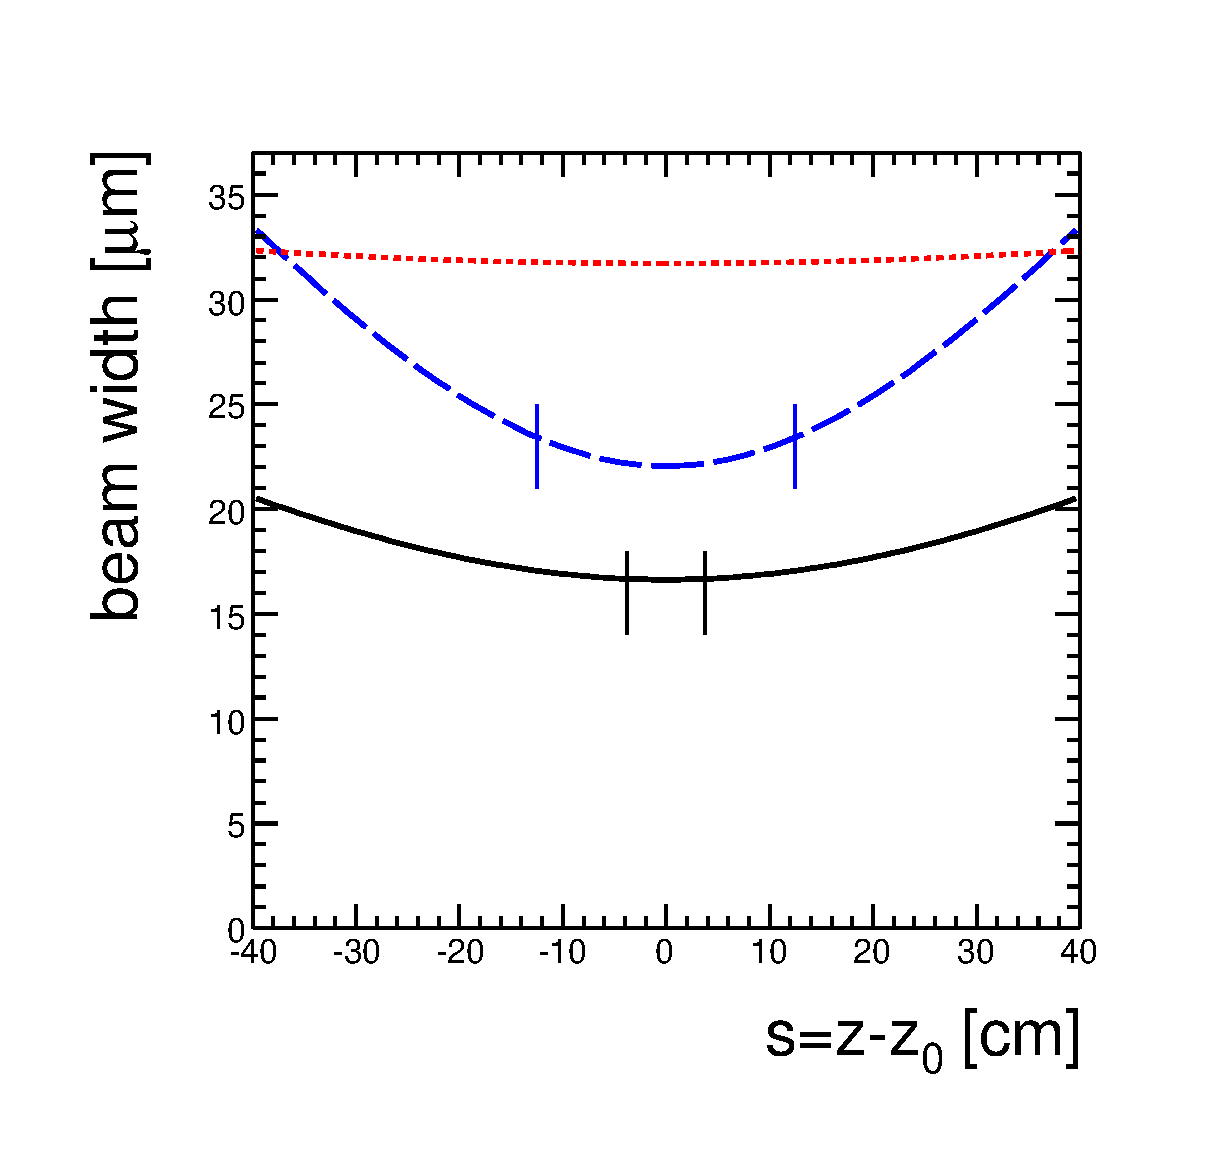
\includegraphics{figures/fxy_beta_functions.eps}}
    \caption{\it Width of the beam as a function of $z$ in cm for three different beam scenarios . The
      solid (black) line corresponds to the nominal LHC configuration. The fine
      dashed (red) line is a LHC fat beam at $\beta^*=200$~cm and 
      $\epsilon=3.75\times 10^{-8}$~cm. The dashed (blue) line corresponds to the 
      Tevatron Run II beam configuration. The marks show the RMS of the collision region.}
    \label{fig:beta_functions}
  \end{center}
\end{figure}


\newpage
\subsection{\label{sec:resol}Tracking detector resolution scenarios}

The five parameter description of a track helix is: 
($C$,$\varphi_0$,$d_0$,$\cot\theta$,$z_p$)

where:\\
\begin{tabular}{lcl}
$C$         &:& is the half curvature of the track (same sign as the charge of the particle)\\
$\varphi_0$ &:& is the direction of the track at point of minimum approach.\\
$d_0$         &:& is the signed impact parameter distance between helix and origin at minimum approach.\\
$\cot\theta$ &:& is the cotangent of the polar angle at minimum approach.\\
$z_p$       &:& is the z position at minimum approach.\\
\end{tabular}

Two CMS detector configurations, as derived from full GEANT 4 simulations, are considered in this note: with pixels (see Ref.~\cite{PhysTDCVol1} page 256) and 
without pixels (Ref.~\cite{PhysTDCVol1} page 256 and Ref.~\cite{IPnopixel}) in 
the tracking system. To be precise the configuration without pixels means the Pixel detector is in place but it is not being read out and therefore no pixel measurements 
contribute to the track fit. The material of the pixel layers still contributes to the multiple scattering and energy loss and therefore has to be taken into account. 
These two detector configurations have very different resolutions 
on the track parameters most relevant to the beam profile calculation: impact 
parameter $d_0$, $\varphi_0$ and  $z_0$.  The resolution function was parameterized as function of $p_T$ (in GeV/c), ignoring any polar angle dependence, 
\begin{equation}
 \label{ptpara}
\sigma^{tr}_{d0} = c_0 + \frac{c_1}{p_T}.
\end{equation} 
The parameter values are listed in Table ~\ref{IPresolution} 
for $d_0$,  $\varphi_0$ and  $z_0$ for both scenarios.   For comparison, resolutions from the CDF-II-like detector are also listed.

\begin{table} [th]
\begin{center}
 \caption{\it \label{IPresolution} Resolution functions of two CMS detector configurations. For comparison, resolutions from the CDF-II-like detector are also listed.}
\vspace{0.5cm}
\begin{tabular}{|c|c|c|c|} \hline
configuration   &     CMS  with Pixel      &  CMS without pixel  & CDF-II\\ \hline
$d_0$           &  $10 + 90/p_T$ ($\mu$ m)  & $100 + 900/p_T$ ($\mu$m) & $11 + 10/p_T$ ($\mu$m) \\ \hline
$\varphi_0$     &  $0.00011 + 0.00190/p_T$~(rad)    & $0.00023 + 0.00580/p_T$~(rad) & $0.0003$~(rad) \\ \hline
$z_p$           &  $0.0017 + 0.0084/p_T$~(cm)       & $0.017 + 0.084/p_T$~ (cm) & 0.5~ (cm)  \\  \hline 
 \end{tabular}

 \end{center}
\end{table}




\section{\label{sect:generator}Data Generation}
\subsection{\label{sec:fast_parameterized_MC}Fast parameterized Monte Carlo simulation using  \root  \texttt{TPythia}}
The parameterized  Monte Carlo simulation uses the \root  \texttt{TPythia} class \cite{pythia6}, which provides a C++ interface to the F77 version of
 the \pythia 6.319  event generator~\cite{pythia}. This allows the  fast  generation of large data sets 
with different beam parameters and tracking scenarios. 
On an AMD64 (32Bit OS), the rate is 162 events/sec for minimum bias events compared to rates 
of the order of one event per minute for the full simulation. In the current form, the fast parameterized Monte Carlo simulation does not include any  pattern recognition effects.   
\pythia creates interactions at the origin of the coordinate system. Final state charged particles are selected and  the event vertex is distributed  
according to Equation (\ref{betafunction}); offsets in $x$ and $y$ are applied and the beam can  have a slope in $x$ and $y$ with respect to the detector axis. 
Then  the vertex and momentum information of these particles is transformed into helix track parameters.

The track parameters of interest are then resolution smeared according to the different track resolution scenarios 
described in Section \ref{sec:resol}. 

Two sets of \pythia control cards were used:
\begin{enumerate}
\item Minimum bias.
\item QCD event with minimal  parton $E_T$ of 50 GeV/c.
\end{enumerate} 
More detail about the control cards can be found in Appendix 2.
The rapidity and transverse momentum  distributions of 
charged tracks are shown in Figure \ref{fig:pythia} for 10000 $pp$ collisions for the two PYTHIA sets. The minimum bias events have very low 
multiplicity, yielding only 1 track with  $p_T > 1.5 $ GeV/c per event 
compared to about 7 such tracks for the events with the minimum parton $E_T$ requirement. 


\begin{figure}[hbtp]
  \begin{center}
    \resizebox{15cm}{!}{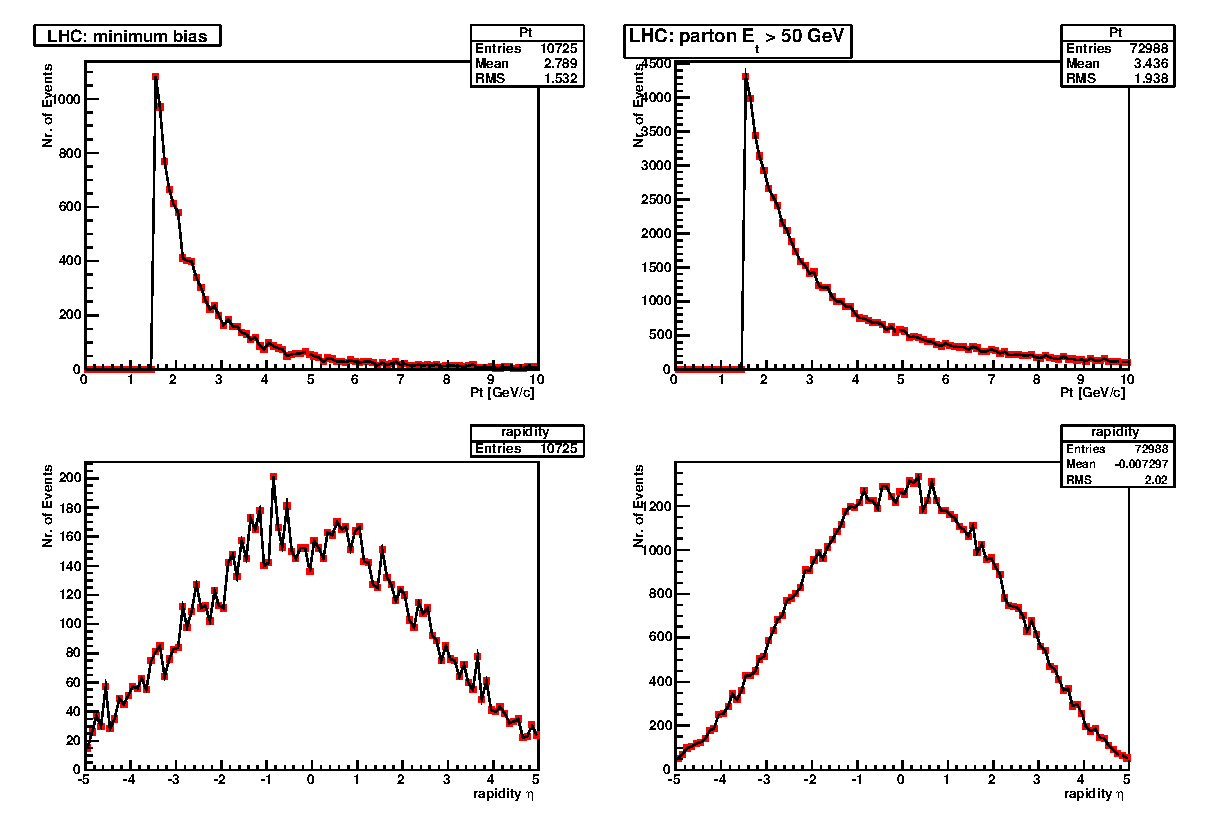
\includegraphics{figures/pythia.eps}}
    \caption{\it Rapidity and $p_T$ distribution of charged tracks for minimum bias events (left) and for events with a minimum parton $E_T>$50 GeV (right) 
                at $\sqrt{s}=$ 14 TeV. Only tracks with  $p_T> 1.5$ GeV/c are considered.}
    \label{fig:pythia}
  \end{center}
\end{figure}


%The results of the vertex displacement at $(300,600,0)$ $\mu$m and the scatter plot of the impact parameter versus
%the angle $\phi$ is shown in Figure~\ref{fig:d0_phi} (a) and (b). For this sample, the 
%nominal LHC 2008 beam configuration was used.
%\newpage   
\subsection{\label{sec:full_MC}Full detector simulation and track reconstruction using \texttt{CMSSW}}
In this case the full detector simulation based on GEANT 4 and the full reconstruction 
within the \texttt{CMSSW} framework is used to generate and reconstruct events. This gives a more 
realistic simulation, including pattern recognition effects, noise hits, non-Gaussian tails etc. Tracks from the Combinatorial Track Finder (CTF) \cite{CTF} collection were used.
The track selection requirements for fully reconstructed tracks are listed in Table \ref{TrackSelection}.

The fully reconstructed samples used are QCD samples for several $\hat{p}_t$ bins and no pile-up, a QCD sample with low luminosity pile-up
($2\times10^{33}cm^{-2} s^{-1}$), an inclusive $b\bar{b}$ sample,
and an inclusive $t\bar{t}$ sample. The QCD samples consist mainly of prompt tracks emanating from the primary interaction vertex, while  $b\bar{b}$ and $t\bar{t}$ samples contain a significant amount of tracks with non-zero impact parameter  stemming from displaced b-decays. We demonstrate that the $d_0-\varphi_0$ fitter
is insensitive to the sample composition. QCD samples with displaced beam spots were also produced (see Table \ref{d0phiresultsfullsim}). 

In order to simulate a more realistic beam profile, a vertex smearing software module~\cite{VtxSmearingPkg}
based on the $\beta$-function was included. This smearing module displaces the vertex given by the
generators using the $\beta$-function for the transverse coordinates and a Gaussian 
distribution for the longitudinal coordinate. This module also allows  the beam to have slopes
$\frac{dx}{dz}$ and $\frac{dy}{dz}$ with respect to the $z$-axis. The following parameters can be varied:

\begin{itemize}
\item \texttt{X0}, \texttt{Y0}, and \texttt{Z0}, where the default values are $(0,0,0)$ $\mu$m. 
\item \texttt{SigmaZ} ($\sigma_z$) with the default of 7.55 cm 
\item \texttt{dx/dz} and \texttt{dy/dz} where the default is 0 $\mu$m/cm . 
\item \texttt{BetaStar} ($\beta^*$) with a default of 55 cm. 
\item \texttt{Emittance} ($\epsilon$) with a default of $3.75\times10^{-8}$ cm. 
\end{itemize}
 
%The tracks from the Combinatorial Track Finder (CTF) \cite{CTF}  collection The track selection requirements for fully reconstructed tracks are 
%listed in Table \ref{TrackSelection}



%\begin{itemize}
%\item Number of hits on silicon strips $>$ 7.
%\item Number of hits on pixel layers $>$ 1.
%\item $\chi^2/ndof  < 5$.
%\item $p_T$ $>$ 2 GeV/c.
%\item $\sigma_{d0} < 150$ $\mu$m.
%\end{itemize}
 

%\clearpage

\begin{table} [th]
\begin{center}
 \caption{\it \label{TrackSelection} Track selection requirements for fully simulated and reconstructed tracks.}
\vspace{0.5cm}
\begin{tabular}{|l|l|} \hline
Silicon Strip Hits                            &  $>$ 7          \\ \hline
Pixel Hits                                    &  $>$ 1          \\ \hline
$\chi^2/ndof$                                 &  $<$ 5          \\ \hline
transverse momentum ($p_T$)                   &  $>$ 2 GeV/c    \\ \hline
impact parameter uncertainty  ($\sigma_{d0}$) &  $<$ 150 $\mu$m \\ \hline
 \end{tabular}

 \end{center}
\end{table}



%\clearpage

%\section{\label{sec:fitters}Description of the various {fitting} routines}
%
%This Section describes the different fitting routines that were used to obtain the results presented in this note. 
%All of the algorithms are track based, which  means every selected track contributes. For this algorithms a determination of the primary vertices 
%is not necessary and they  require less data than fits based on reconstructed primary vertices. The algorithms are expected to be insensitive to 
%Pile Up contributions, since it does not matter if the track emanates from the hard collision or from Pile Up.
%The various fitters were integrated into the CMS offline framework 
%\cite{BeamSpotProducer}, but are also available as stand alone routines \cite{CVS}. 

%\clearpage 
\section{\label{sec:dphi}The $d_0-\varphi_0$ fitter}

This fit is both fast and robust and has been in use by CDF for many years (see e.g. \cite{NIM}) to estimate the beam positions both on-line 
and off-line. Within the CMS experiment, this fitter has also been initially studied \cite{oldCMSnote}.
Many physics analysis use the beam position calculated 
by this method as a precise unbiased estimate of the primary interaction vertex. 
This fitting method is also used to get the initial parameters for the other fitters described in Section~\ref{sec:width}.
A determination of the primary vertices 
is not necessary for this algorithm and less data than fits based on reconstructed primary vertices is required. The algorithms are expected to be insensitive to 
pile up contributions, since it does not matter if the track emanates from the hard collision or from pile up.
The various fitters were integrated into the CMS offline framework 
\cite{BeamSpotProducer}, but are also available as stand alone routines \cite{CVS}. 

\begin{figure}[htp]
  \centering
    \subfigure[]{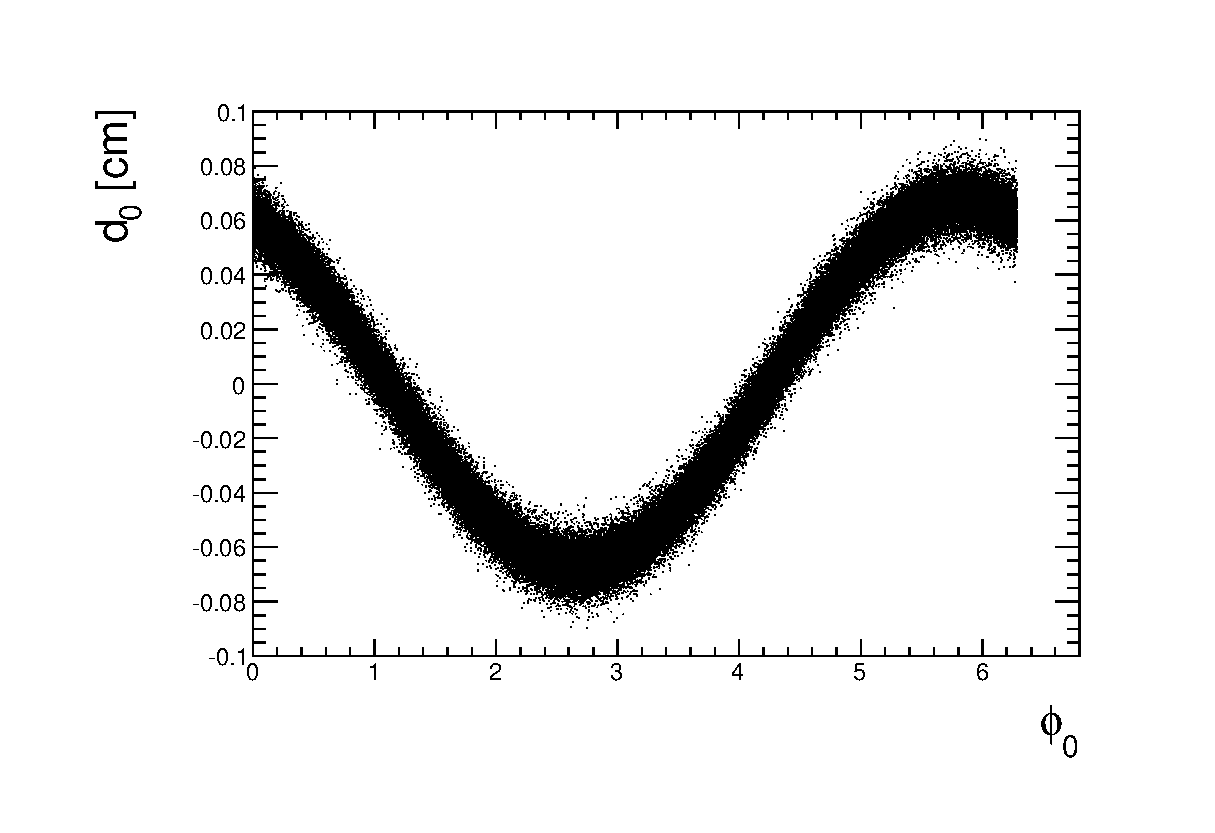
\includegraphics[width=0.45\textwidth]{figures/fxy_d0_phi.eps}}
    \subfigure[]{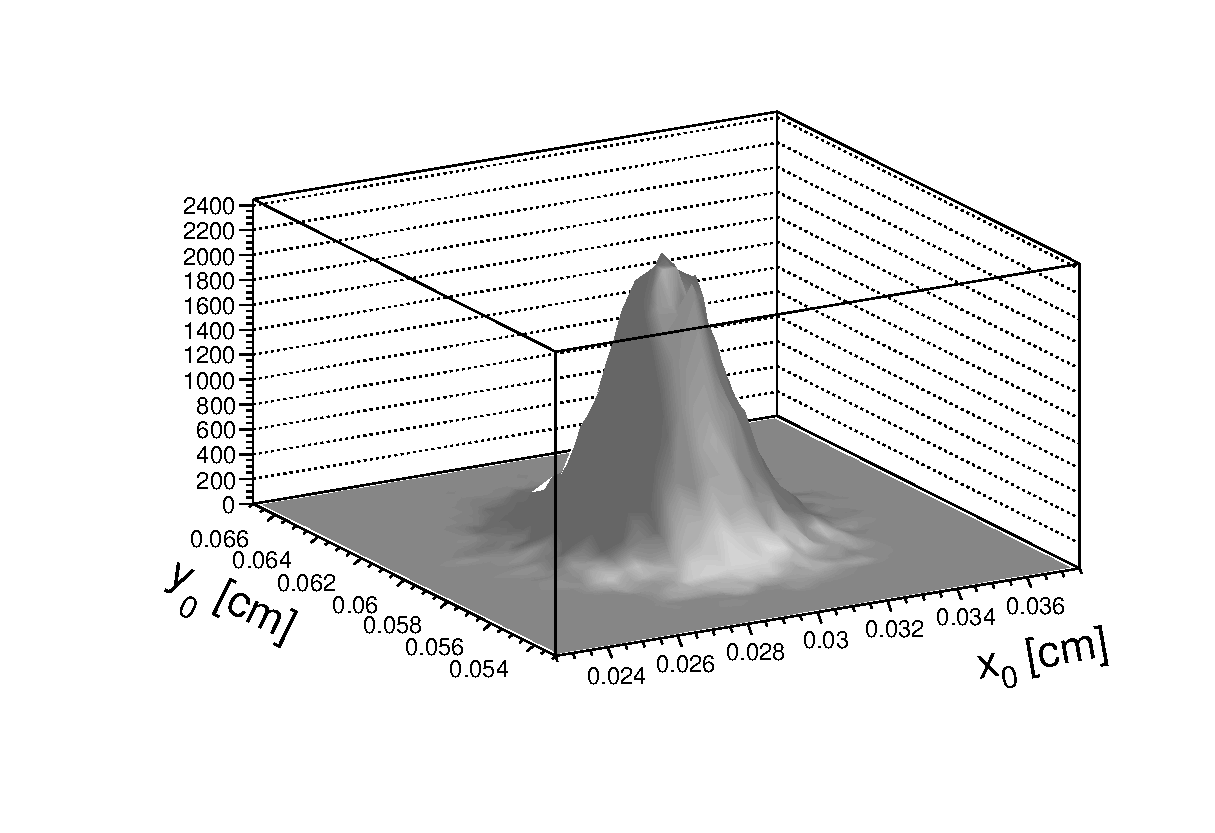
\includegraphics[width=0.45\textwidth]{figures/fxy_x0_y0_scatter.eps}}
    \subfigure[]{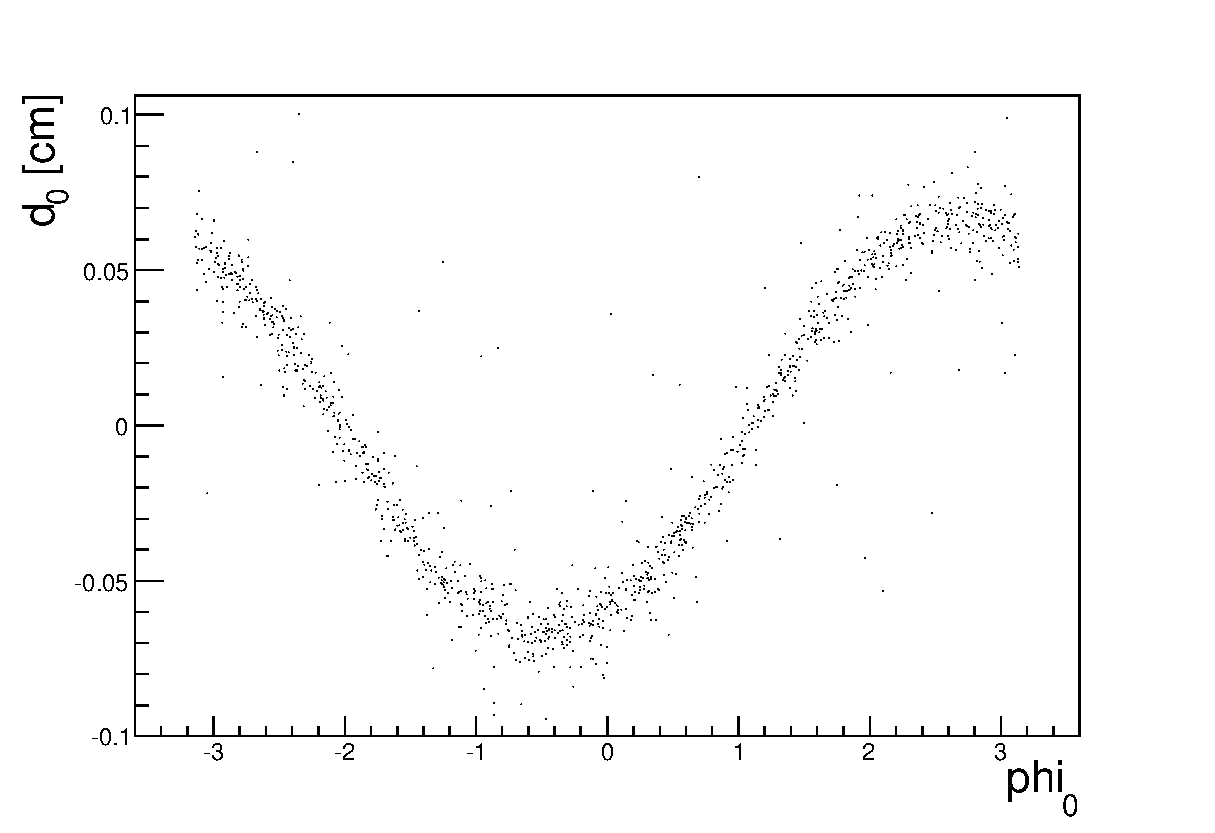
\includegraphics[width=0.45\textwidth]{figures/fxy_reco_d0_phi.eps}}
    \subfigure[]{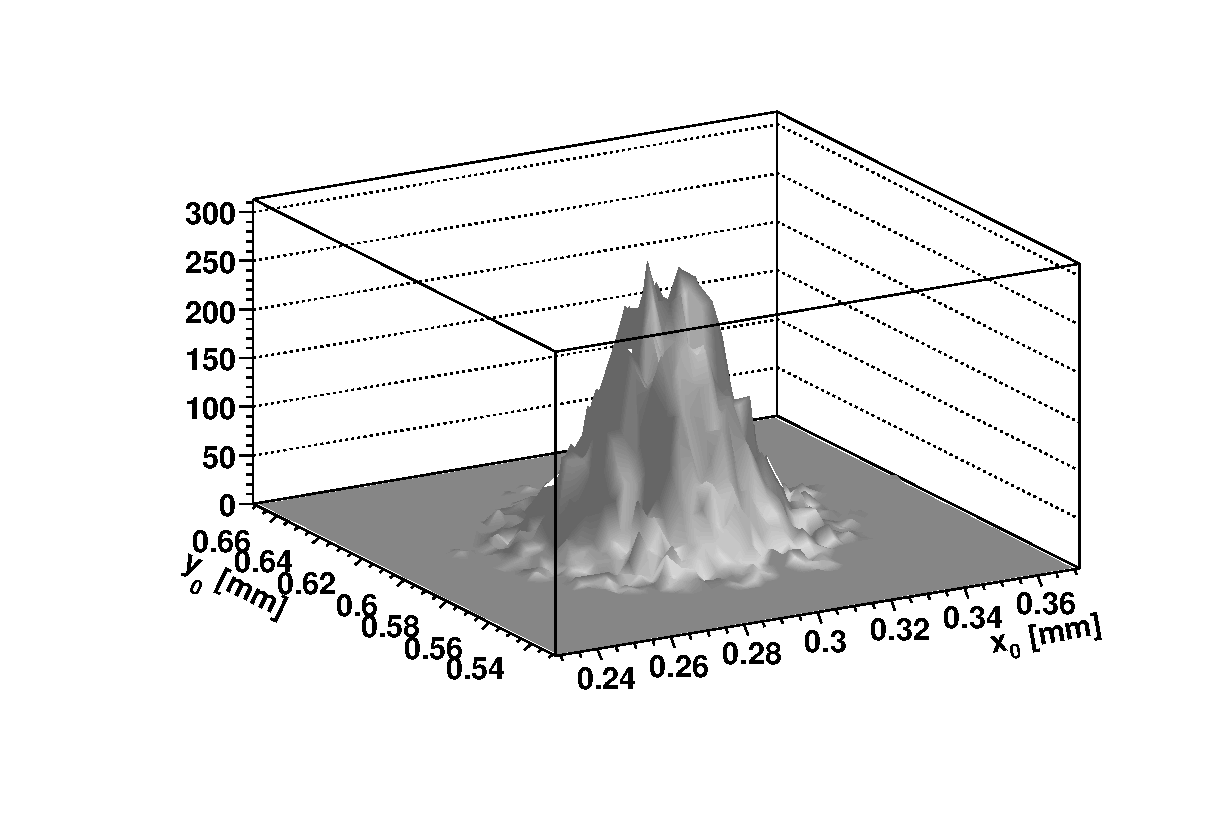
\includegraphics[width=0.45\textwidth]{figures/fxy_reco_x0_y0_scatter.eps}}
      
    \caption{\it (a) Correlation between $d_{0}$ and $\varphi_{0}$ for a displaced beam 
      given by the stand alone generated sample. In this example the displacement 
      of the beam with respect to the detector coordinate system is  $x_0$ =
      300 $\mu$m and  $y_0$ = 600 $\mu$m (no slope in $x$ and $y$). We 
      observe a sine function where the amplitude is given by $\sqrt{x_0^2 +y_0^2}=734$
      $\mu$m and the phase is shifted by $\varphi_0=tan\left(\frac{y_0}{x_0}\right) = 1.1 $ radians. (b) Shows the transverse beam profile for the stand alone generated sample.
      (c) Correlation between $d_0$ and $\varphi_0$ for selected tracks from full simulation and reconstruction.
      (d) Transverse beam profile from the full simulation.
    }
    \label{fig:d0_phi}
\end{figure}



The variation of the impact parameter of all tracks is shown in  Figures \ref{fig:d0_phi}(a) and  \ref{fig:d0_phi}(c) as  a function of $\varphi$ when 
the beam is displaced with respect to the detector coordinate system. The transverse 
beam profile is shown in Figures \ref{fig:d0_phi}(b) and \ref{fig:d0_phi}(d). 
Figures~\ref{fig:d0_phi}(a) and ~\ref{fig:d0_phi}(b) correspond to a high statistics sample obtained with the fast Monte Carlo simulation  
described in Section~\ref{sec:fast_parameterized_MC}.
The distributions corresponding to the fully simulated sample of 3000
minimum bias events are shown in Figures ~\ref{fig:d0_phi}(c) and (d). The total number of tracks, selected by the requirements listed in Table \ref{TrackSelection}, is 1268.



This correlation is used to extract the beam parameters. 
To first order, the impact parameter $d_0$ for tracks coming from the primary 
vertex can be parametrized by

\begin{equation}
d_{0}(\varphi_0,z_p) = x_0 \cdot \sin\varphi_0 + \frac{dx}{dz} \cdot \sin\varphi_0 
\cdot z_p - y_0 \cdot \cos\varphi_0 - \frac{dy}{dz} \cdot \cos\varphi_0\cdot z_p  ,
\end{equation}

\noindent
where $x_0$ and $y_0$ are the position of the beam at $z = 0$, and
$\frac{dx}{dz}$ and $\frac{dy}{dz}$ are the $x$ and $y$ slopes of the beam.


\noindent
The $d_0 - \varphi_0$ fitter is a simple iterative $\chi^2$ fitter.   
The contribution from each track is weighted by its error. %Ignoring the correlation between $ d_{0}, \varphi_0$ and $z_0 $, 
The $\chi^2$ distribution to be minimized is

\begin{equation}
\chi^2  = \sum_{i=1}^{N_{Tracks}} \left( \frac{d_{0i}-(x_0 \cdot \sin\varphi_{0i} + \frac{dx}{dz} \cdot \sin\varphi_{0i} 
\cdot z_{pi} - y_0 \cdot \cos\varphi_{0i} - \frac{dy}{dz} \cdot \cos\varphi_{0i}\cdot
z_{pi})}{\sigma_i} \right)^2 ,
\end{equation}
where $\sigma_i^2 = \sigma_{d0}^2 + 2\cdot\sigma_{Beam}^2$, and $\sigma_{Beam}$ is the average transverse beam width. 
%\footnote{The factor 2 comes from the assumption that 
%the error on $x$ and $y$ are similar.} 


Using a vector notation, the $\chi^2$ function can be written as

\begin{equation}
\chi^2  = \sum_{i=1}^{N_{Tracks}} \left( \frac{d_{0i}-(\vec{x}\cdot\vec{g_i})}{\sigma_i}
 \right)^2,
\end{equation}


\noindent
where $\vec{x} = (x_0,y_0,\frac{dx}{dz},\frac{dy}{dz})$ and 
$\vec{g_i} = ( \sin\varphi_{0i}, -\cos\varphi_{0i},\sin\varphi_{0i} \cdot z_{pi}, 
-\cos\varphi_0\cdot z_p)$.


\noindent
The solution for $\vec{x}$ is then

\begin{equation}
\vec{x}= V \cdot \vec{sg},
\end{equation} 

\noindent
where the inverse of the 4 $\times$ 4 matrix $V$ is given by

\begin{equation}
V^{-1}_{lm} = \sum_{i=1}^{N_{Tracks}}\frac{g_{il} \cdot g_{mi}}{\sigma_i^2},~~(l,m = 1,2,3,4)
\end{equation} 


\noindent
and the vector $\vec{sg}$ 

\begin{equation}
sg_l = \sum_{i=1}^{N_{Tracks}} \frac{g_{li} \cdot d_{0i}}{\sigma_i^2}, ~~(l = 1,2,3,4).
\end{equation} 
Tracks must initially pass a set of basic quality requirements.
From this set, tracks that have a large contribution to   
the total $\chi^2$ ($\Delta \chi^2 > \Delta\chi^2_{cut}$) or tracks which 
have a large impact parameter with respect to the fitted beam line  
($|d'_0| > D_{cut} $) are removed until a given fraction of the tracks remain.
All initially selected tracks are evaluated at each iteration. A track that 
was rejected in a previous iteration can enter the next iteration
as the estimate of the beam position improves. In this way, no bias is introduced stemming from a bad initial fit. 
In this note an initial value  $D_{cut}$ = 4.0 cm was used, and this selection was tightened at each iteration, $D^{n+1}_{cut}= D^{n}_{cut}/1.5$, until 
about 50\% of the initially selected tracks survive. The choice of  this parameters is not optimized but also not very critical. 


As more tracks are included in the fit, the convergence to the generated values is observed in Figure \ref{fig:x0_and_y0_dphi_fit}.
A statistical precision of about 2  $\mu$m for $x_0$ and $y_0$  and $\approx 0.2$ $\mu$m/cm for the slopes is achieved with 1000 tracks.
This study was done using the fast parametrized Monte Carlo simulation with pixels described in Section ~\ref{sec:fast_parameterized_MC}.




\begin{figure}[htp]
  \centering
    \subfigure[]{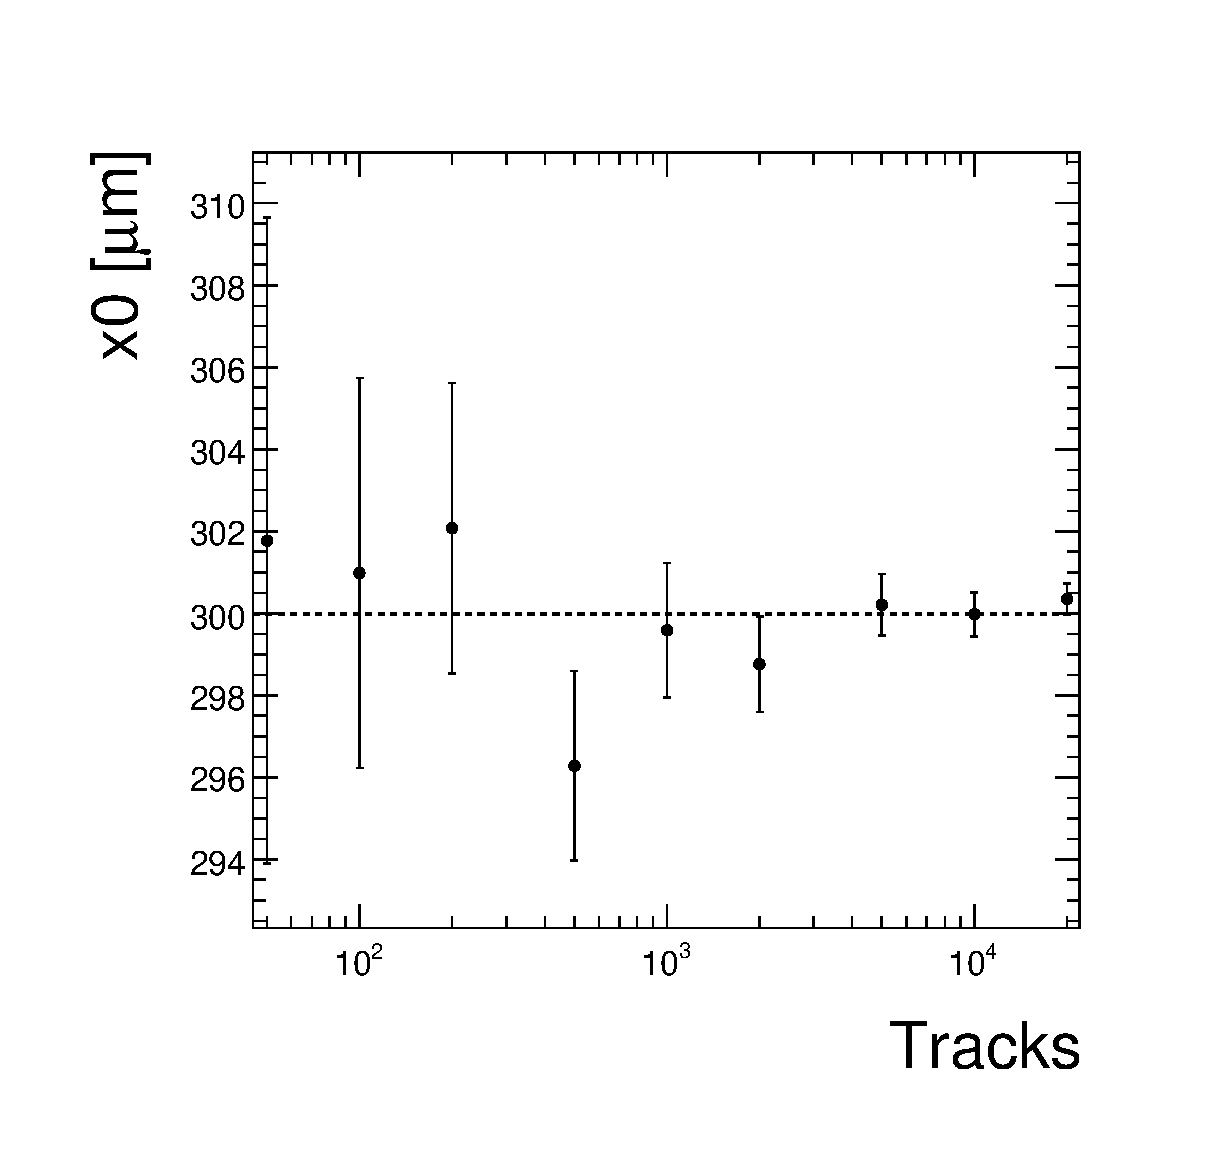
\includegraphics[width=0.45\textwidth]{figures/fxy_x0dphi_fit.eps}}
    \subfigure[]{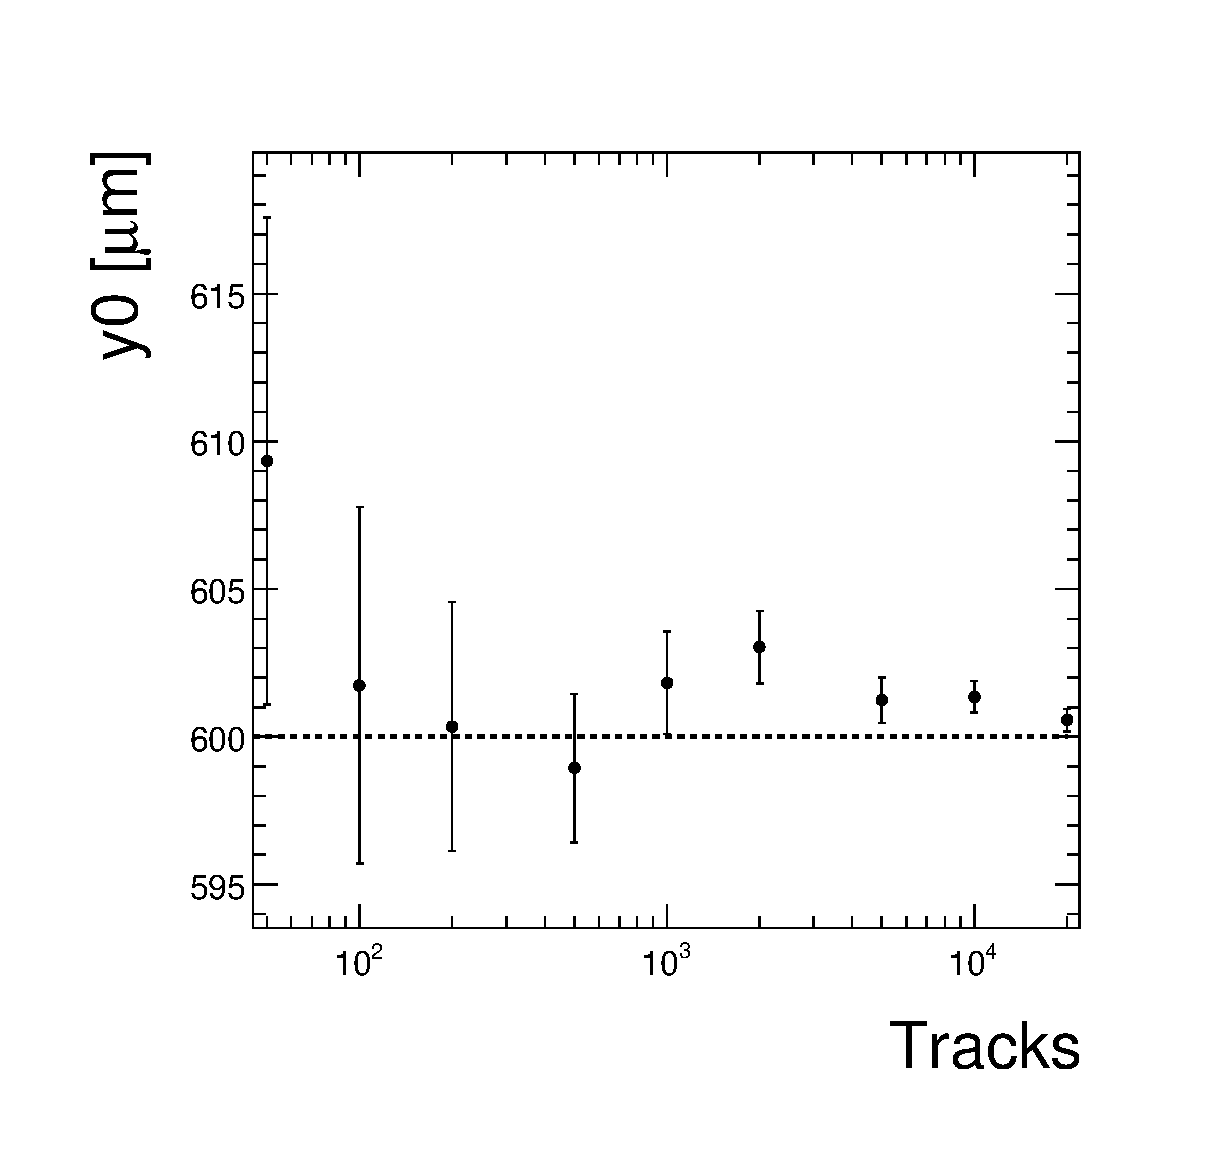
\includegraphics[width=0.45\textwidth]{figures/fxy_y0dphi_fit.eps}}      
    \subfigure[]{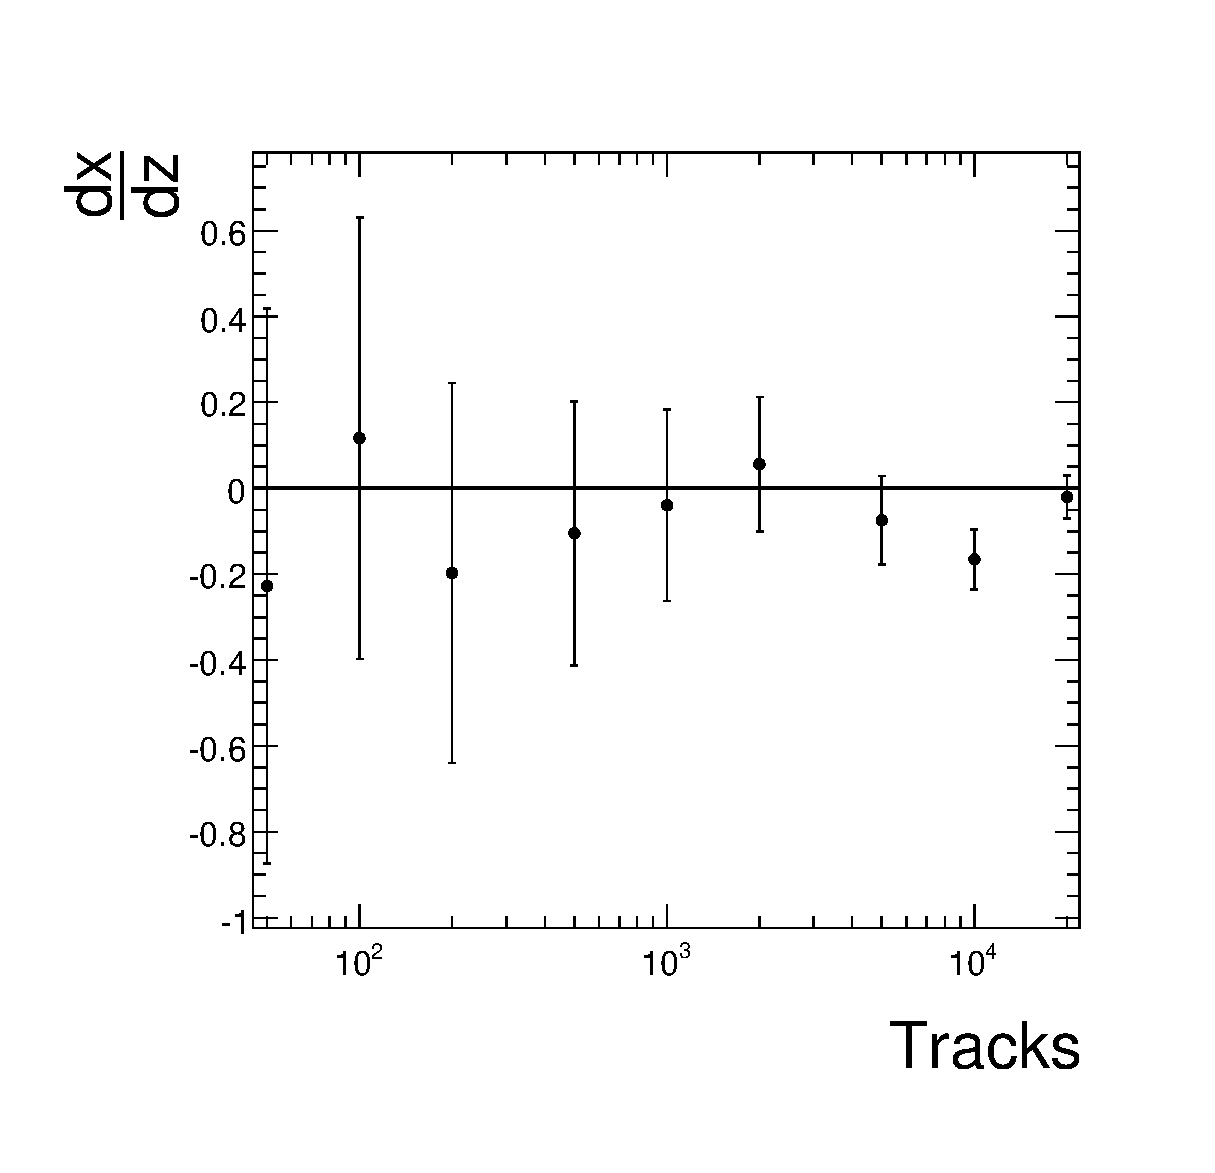
\includegraphics[width=0.45\textwidth]{figures/fxy_dxdphi_fit.eps}}
    \subfigure[]{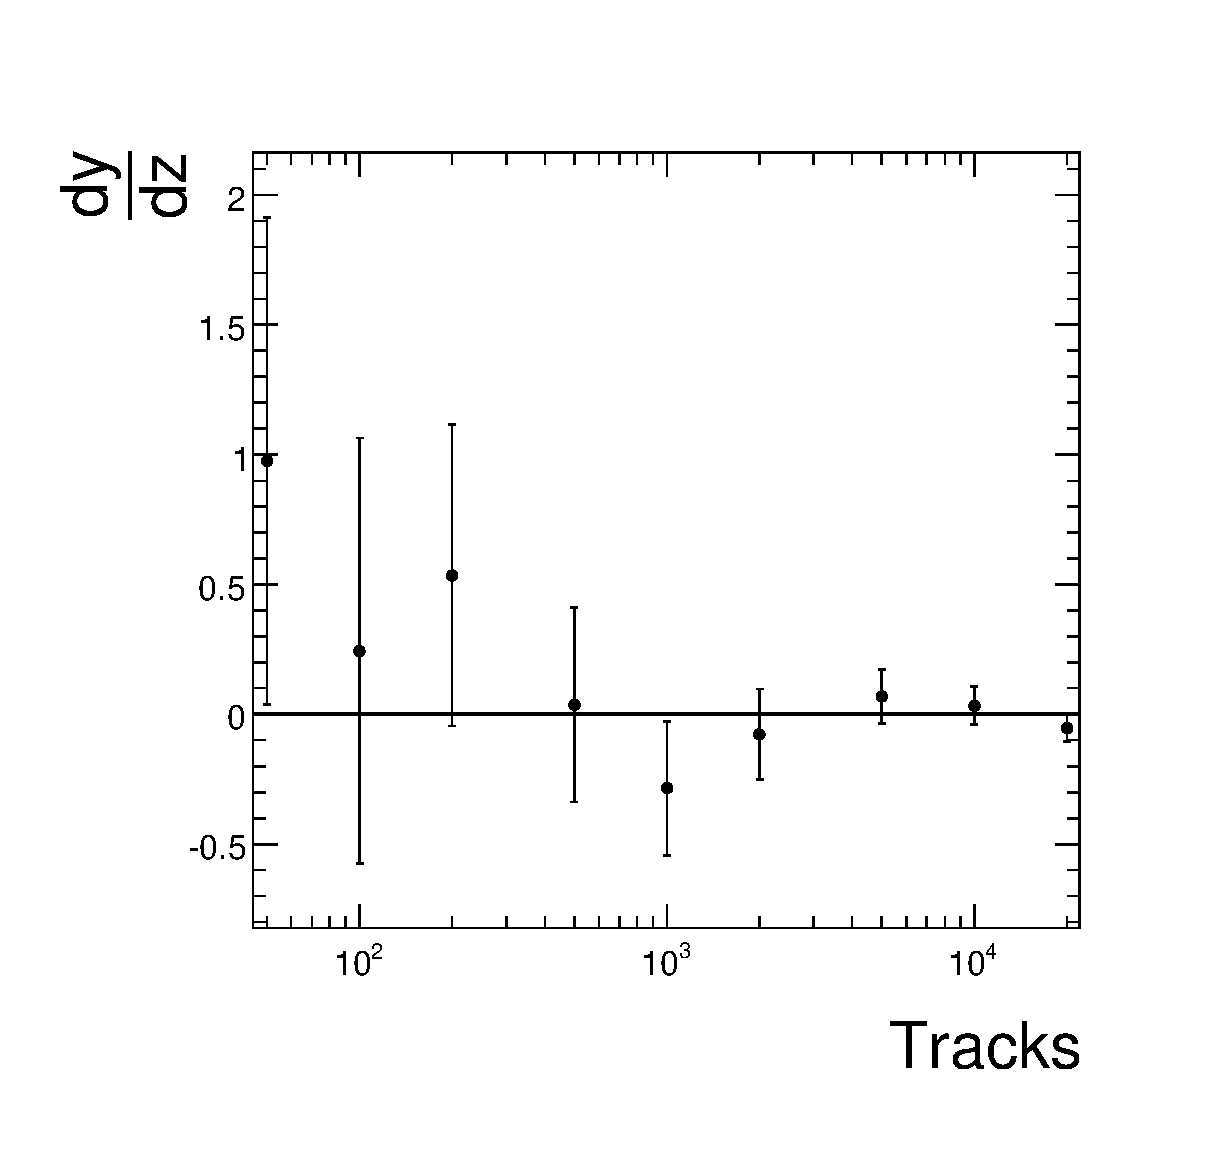
\includegraphics[width=0.45\textwidth]{figures/fxy_dydphi_fit.eps}}      
    \caption{\it    $d_0-\varphi_0$ fit results for (a) $x_0$, (b) $y_0$, (c) $\frac{dx}{dz}$ and (d) $\frac{dy}{dz}$  as a function of the number of tracks.
 Only 1000 tracks are needed to achieve a 2 $\mu$m statistical precision for the beam position. This study was done using the fast parametrized Monte 
Carlo simulation with pixels described in Section ~\ref{sec:fast_parameterized_MC}.  }
    \label{fig:x0_and_y0_dphi_fit}

\end{figure}

The results of the $d_0-\varphi_0$ fitter for different
fully simulated and reconstructed samples consisting of 500 events each 
are shown in Table~\ref{d0phiresultsfullsim}. In each case, the fit converges to a value 
within 2-3 $\mu$m of the value used to generate the sample.  

%This samples  include an inclusive $t\bar{t}$
%sample with displaced vertices from b-decays and a sample with contributions from Pile Up (PU) 
%as expected for low luminosity running ($2\times10^{33}cm^{-2} s^{-1}$). 

 
\begin{table} [th]
\caption{\it \label{d0phiresultsfullsim} Results of the $d_0
- \varphi_0$ fit for several
fully simulated and reconstructed samples with 500 events, uncertainties are statistical only.}
\begin{center}
\small
\begin{tabular}{|c|c|c|c|c|c|c|c|} \hline
Sample & Iteration & selected Tracks           & $x_0$ [$\mu$m] &
$y_0$ [$\mu$m] & $dx/dz$ [$\times10^{-6}$] & $dy/dz$
[$\times10^{-6}$] \\ \hline\hline
generated values                  &     &       & $0.0$             & $0.0$             & $0.0$               & $ 0.0$              \\ \hline
QCD                               &  1  & 6892  & $2.30   \pm 0.67$ & $2.17  \pm 0.66$  & $96.05   \pm 12.87$ & $61.92  \pm 12.82$  \\
($80<\hat{p}_T<120$)              & 19  & 4086  & $2.41   \pm 0.94$ & $-0.60 \pm 0.92$  & $44.22   \pm 17.91$ & $-19.98 \pm 17.87$  \\ \hline
QCD                               &  1  & 8824  & $2.06   \pm 0.57$ & $-0.11 \pm 0.56$  & $-10.44  \pm 10.96$ & $-38.23 \pm 10.70$  \\
($120<\hat{p}_T<170$)             & 19  & 5405  & $1.23   \pm 0.77$ & $-0.88 \pm 0.76$  & $-18.09  \pm 15.11$ & $-33.02 \pm 14.54$  \\ \hline
b-jet                             &  1  & 6392  & $0.56   \pm 0.69$ & $0.15  \pm 0.68$  & $233.78  \pm 13.70$ & $29.70  \pm 13.26$  \\
($50<\hat{p}_T<120$)              & 18  & 3431  & $-2.78  \pm 1.06$ & $2.38  \pm 1.07$  & $76.39   \pm 21.34$ & $-46.86 \pm 20.64$  \\ \hline
QCD with PU                       &  1  & 6933  & $-1.16  \pm 0.74$ & $-3.58 \pm 0.74$  & $95.05   \pm 14.35$ & $-35.69 \pm 14.06$  \\
($2\times10^{33}cm^{-2} s^{-1}$)  & 19  & 3845  & $-0.57  \pm 1.06$ & $-1.02 \pm 1.05$  & $-35.08  \pm 20.33$ & $-20.41 \pm 19.83$  \\ 
($50<\hat{p}_T<80$)               &     &       &                   &                   &                     &                \\ \hline
inclusive $t\bar{t}$              &   1 & 10802 & $7.45   \pm 0.50$ & $3.91  \pm 0.49$  & $27.78   \pm 9.30$  & $44.87  \pm 9.21$   \\
                                  & 19  & 5680  & $-0.33  \pm 0.75$ & $0.43  \pm 0.75$  & $-12.94  \pm 13.89$ & $36.57  \pm 14.09$  \\ \hline\hline
generated values                  &     &       & $300.0$           & $600.0$           & $2000.0$            & $1000.0$            \\ \hline
QCD                               &  1  & 2773  & $299.23 \pm 1.01$ & $592.55 \pm 1.10$ & $2004.07 \pm 15.38$ & $986.52 \pm 16.42$  \\
$40<\hat{p}_T$                    & 19  & 1613  & $300.91 \pm 1.39$ & $601.41 \pm 1.53$ & $2023.38 \pm 21.12$ & $993.70 \pm 23.01$  \\ \hline\hline
generated values                  &     &       & $300.0$           &$600.0$            & $150.0$             & $0.0$               \\ \hline
QCD                               &  1  & 2886  & $299.40 \pm 1.05$ & $600.48 \pm 1.03$ & $261.98  \pm 15.83$ & $-11.48 \pm 15.72$  \\
$40<\hat{p}_T$                    & 19  & 1666  & $295.09 \pm 1.51$ & $599.13 \pm 1.44$ & $167.98  \pm 22.35$ & $-5.87  \pm 21.86$  \\ \hline
\end{tabular}
\end{center}

\end{table} 


\begin{table} [th]
\caption{\it \label{d0phiresultsNopixel} Results of the $d_0
- \varphi_0$ fit for the fast simulation with and without pixel detector, uncertainties are statistical only.
In the non pixel case, the $p_t$ cut was raised to $p_t>5$ GeV/c.}
\begin{center}
\small
\begin{tabular}{|c|c|c|c|c|c|c|c|} \hline
Sample         & Generated Tracks  & $x_0$ [$\mu$m] & $y_0$ [$\mu$m] & $dx/dz$ [$\times10^{-6}$] & $dy/dz$ [$\times10^{-6}$] \\ \hline\hline
generated values &     & $300.0$ & $600.0$ & $0.0$ & $0.0$ \\ \hline
with pixels    & 1000  & $299.59 \pm 1.64$ & $601.83 \pm 1.74$ & $-3.93 \pm 22.32$ & $-2.85 \pm 25.76$  \\
with pixels    & 10000 & $299.98 \pm 0.54$ & $601.35 \pm 0.54$ & $-16.57 \pm 7.08$ & $3.36 \pm 7.25$  \\
with pixels    & 20000 & $300.35 \pm 0.38$ & $600.57 \pm 0.38$ & $-2.00 \pm 4.98$ & $-5.39 \pm 5.09$  \\ \hline

non pixels     & 1000  & $296.89 \pm 7.50$ & $605.53 \pm 7.70$ & $-77.29 \pm 98.57$ & $-132.54 \pm 104.35$  \\
non pixels     & 10000 & $299.43 \pm 2.38$ & $597.03 \pm 2.40$ & $-34.80 \pm 31.47$ & $69.42 \pm 32.03$ \\
non pixels     & 20000 & $299.42 \pm 1.89$ & $597.02 \pm 1.90$ & $12.83 \pm 24.88$ & $44.83 \pm 25.36$ \\ \hline
\end{tabular}
\end{center}

\end{table} 


The 90\% confidence limits for the transverse position of the beam are shown in 
Figure~\ref{fig:contours} for the case with pixel (scenario 1) and for the case with
no-pixel (scenario 2). The marker shows the input value used to generate the samples at (300,600,0) $\mu$m. For
scenario (1), 20k tracks are used in the fit while 50k tracks and tightened $p_T$ 
selection are required in scenario (2). In the non pixel case, the $p_T$ cut was raised to $p_T>5$ GeV/c. The average beam position can still be measured with
worse resolution but the beam width cannot be resolved in this case. The results of the fit for both
scenarios running only with the fast simulation is presented in Table~\ref{d0phiresultsNopixel}.


\begin{figure}[hbtp]
  \begin{center}
    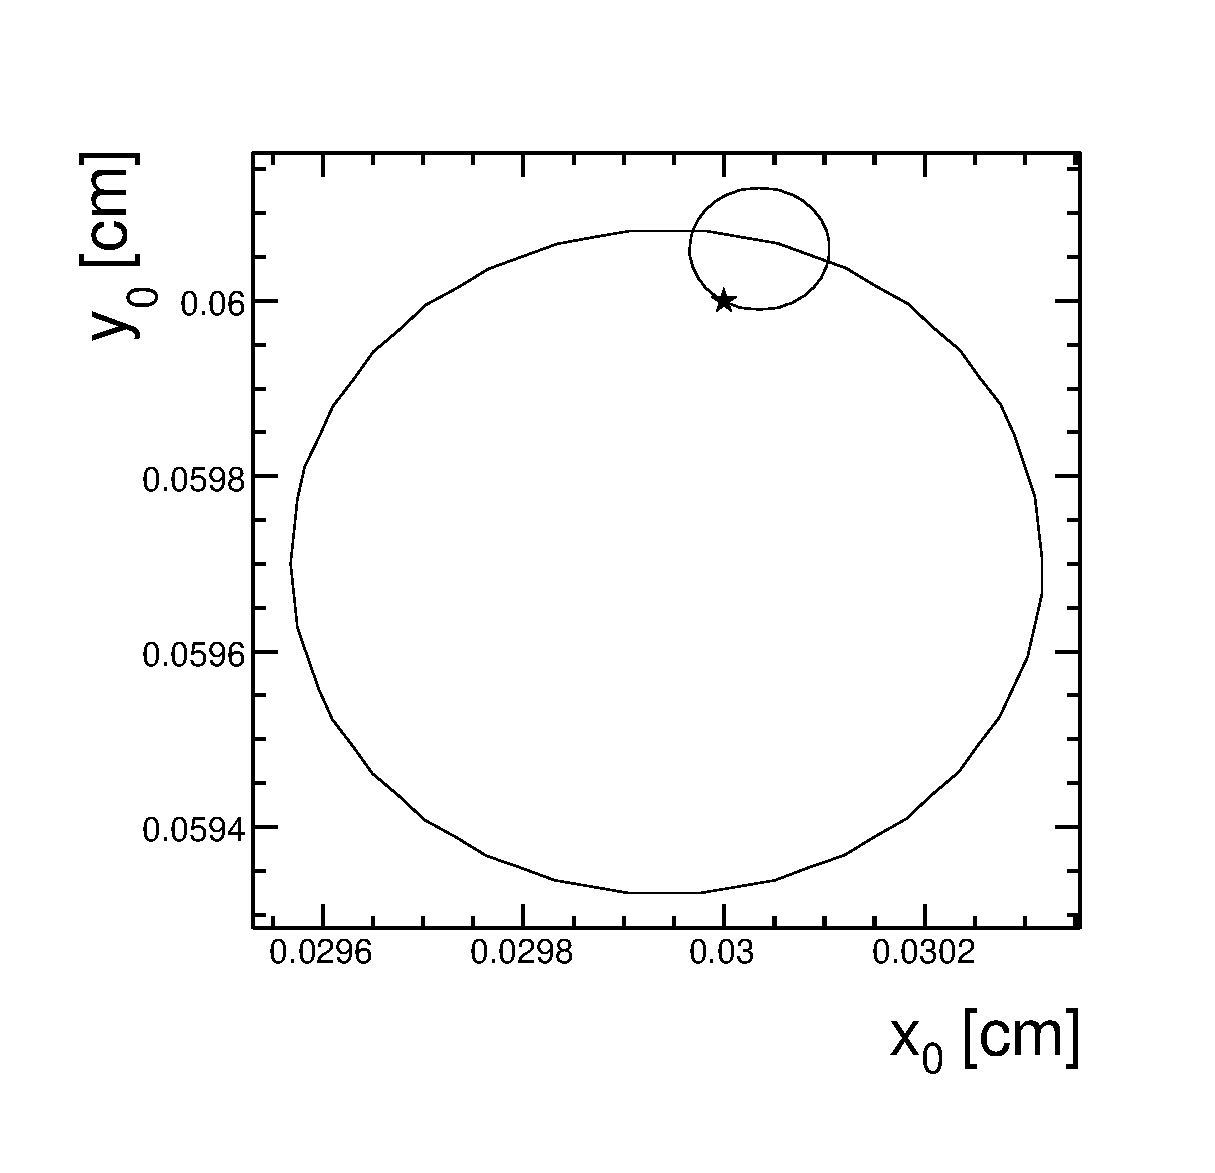
\includegraphics[width=0.5\textwidth]{figures/fxy_contour_x0y0.eps}
    %\subfigure[]{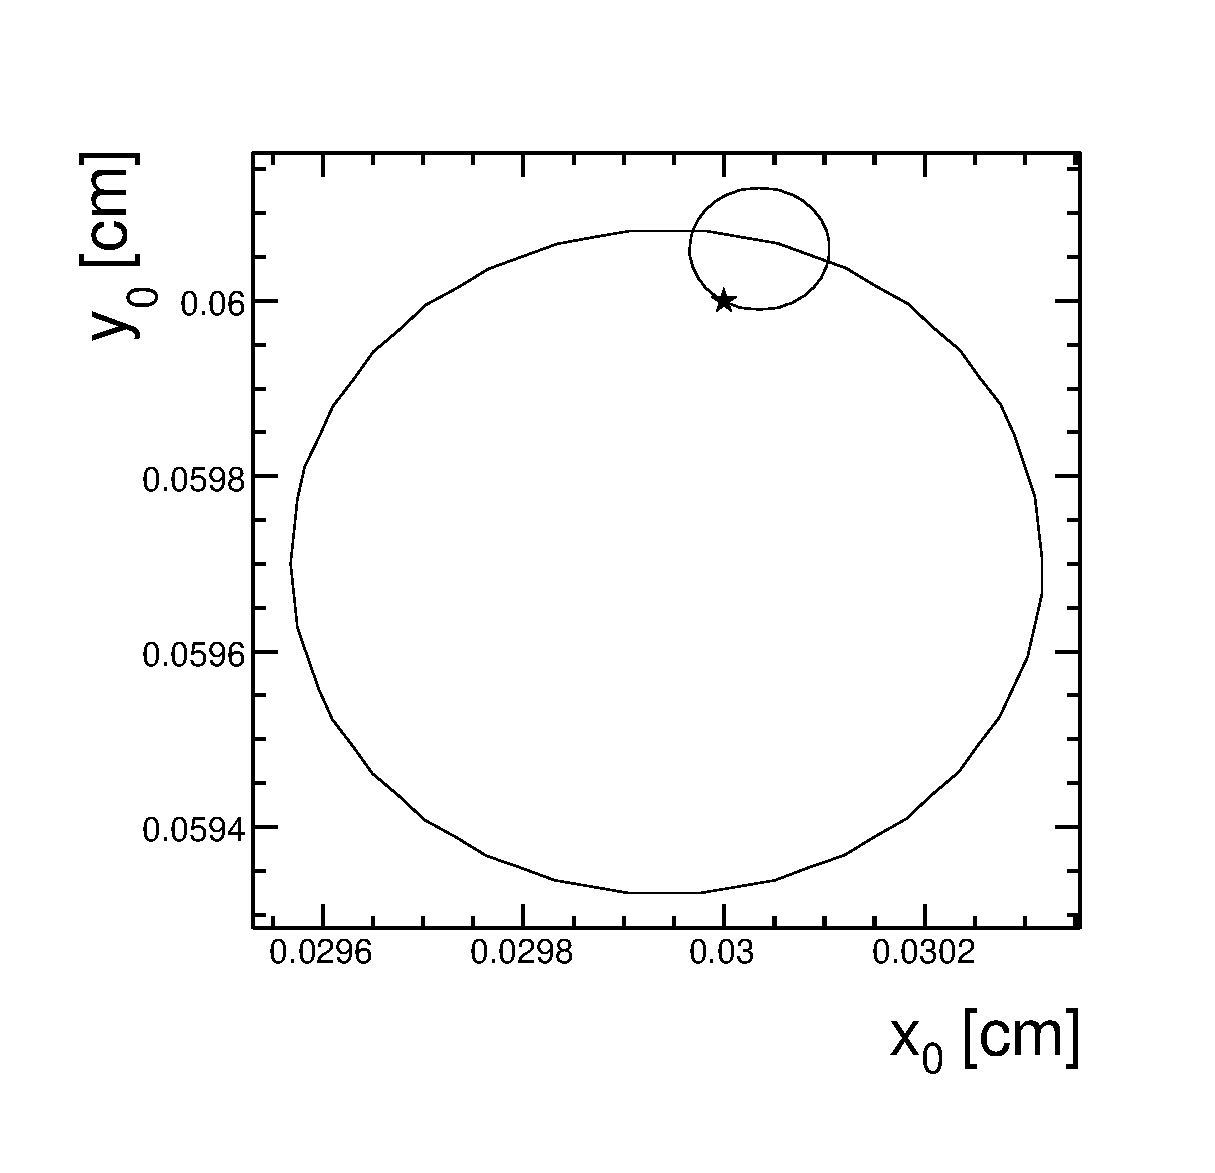
\includegraphics[width=0.45\textwidth]{figures/fxy_contour_x0y0.eps}}
    %\subfigure[]{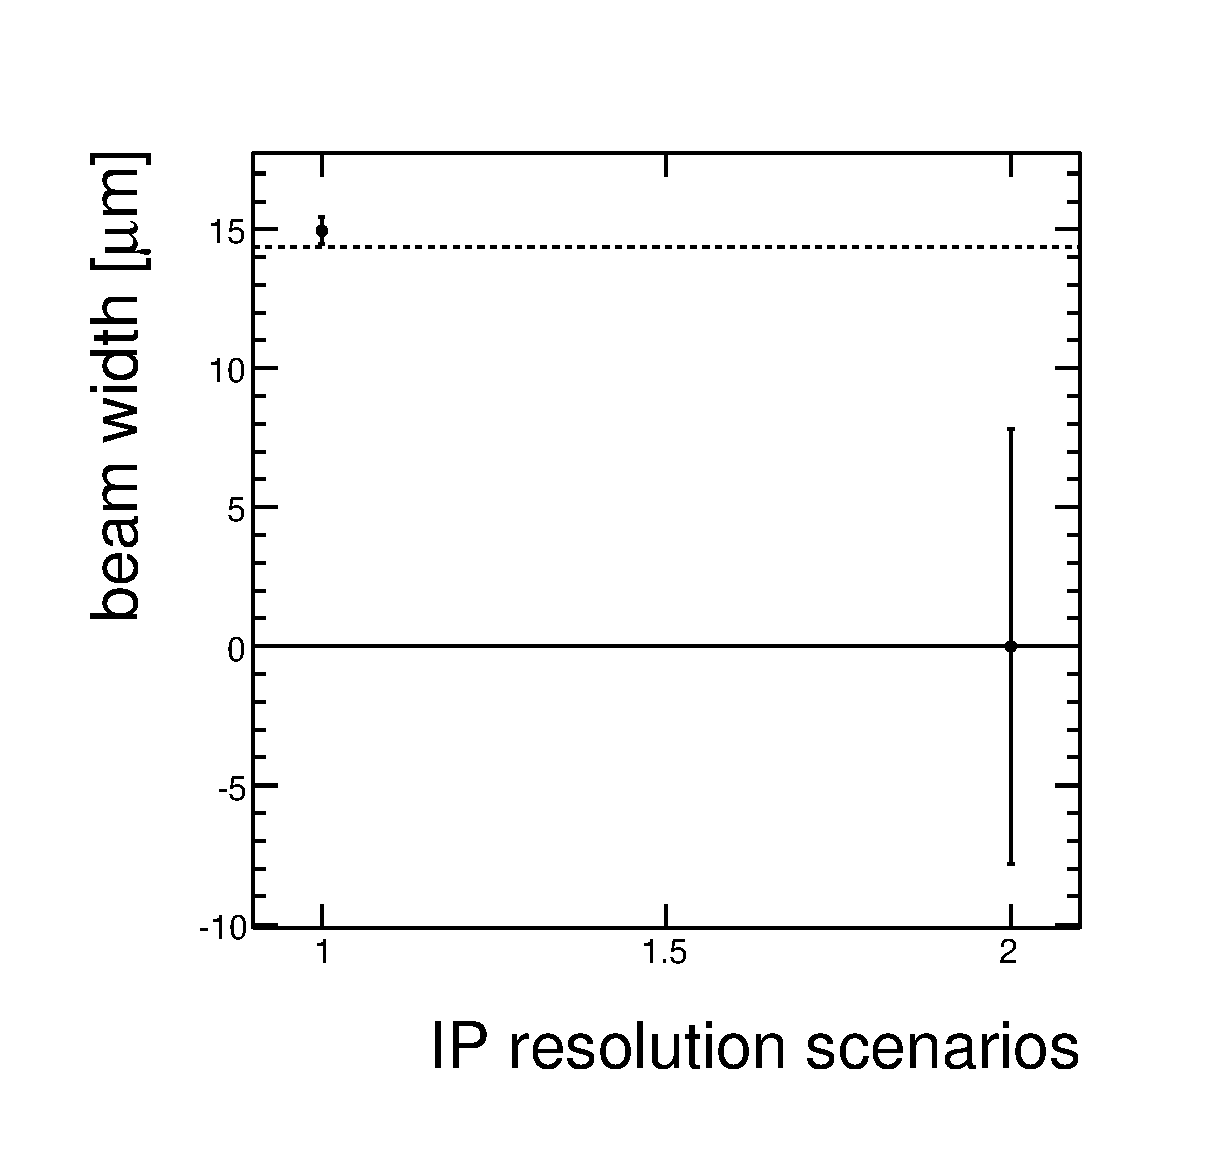
\includegraphics[width=0.45\textwidth]{figures/fxy_beamwidth_vs_resolutions.eps}}
   \caption{\it 90\% CL contours for the transverse beam position with different
     IP resolutions. The marker shows the input value for the generation (300,600,0) $\mu$m. This study was done using the fast parametrized Monte 
Carlo simulation described in Section ~\ref{sec:fast_parameterized_MC}. The big ellipse with a radius of 
approximately 3  $\mu$m corresponds to the no-pixel case while the small ellipse with a radius of less 
than 1  $\mu$m corresponds to the case with pixel detector. }
   \label{fig:contours}
  \end{center}
\end{figure}


\clearpage
\section{\label{sec:additional}Additional Beam Fitters}
In the previous section, the $d_0 - \varphi_0$ fitter was shown to be robust, stable, and to yield good 
results.
In this section, additional fitters are described. These fitters are extensions of the $d_0 - \varphi_0$ 
fitter providing additional information like the transverse beam width or the parameters of the $\beta$-function.  
These fitters are sensitive to several effects like the detector acceptance and require excellent
understanding of the track parameter uncertainties, therefore only a proof-of-concept is given using the 
fast simulation. We only considered the detector configuration with pixels. Without pixels the 
resolution is not sufficient to extract the beam width and $\beta$ function.

\subsection{\label{sec:width}The Log-likelihood {fitter} to extract the beam parameters}


To extract the beam parameters an unbinned log-likelihood fit can be used which treats the contribution of the 
track parameter errors to the probability function event by event.  
The probability function is the product of a longitudinal and a transverse component:
\begin{equation}
P(d'_0,z_p,\sigma_{d0}^{tr},\sigma_z^{tr})=
\frac{1}{\sqrt{2\pi}\sigma_{d'0}(z_p)} e^{-\frac{d'^2_{0}}{2\sigma_{d'0}(z)^2}}
\cdot \frac{1}{\sqrt{2\pi}\sigma_z} e^{-\frac{(z_p-z_0)^2}{2\sigma_z^2}}
\end{equation}

\noindent where $d'_0$ is the impact parameter with respect to the beam given by 

\begin{equation}
\label{eq:dprime0}
d'_0=d_0-(x_0+\frac{dx}{dz}z_p)\sin\varphi_0+(y_0-\frac{dy}{dz}z_p)\cos\varphi_0 . 
\end{equation}

The error on $d'_0$ is 

\begin{equation}
\label{eq:sigmadprime0} 
\sigma_{d'0}(z_p)= \sqrt{ \left( \sigma_{Beam}\right)^2 +(\sigma_{d0}^{tr})^2}, 
\end{equation}

\noindent where $\sigma_{d0}^{tr}$ is the impact parameter resolution of tracks as provided by the track fit.
Assuming  the transverse width of the beam  does not vary much in $z_p$, as will be the  case for the LHC nominal scenario, an
average $\sigma_{Beam}$ can be used. The error on $z_p$ is

\begin{equation}
\sigma_z= \sqrt{(\sigma^{b}_z)^2 +(\sigma_z^{tr})^2},
\end{equation}

\noindent where $\sigma_z^{tr}$ is the $z$ resolution of tracks as returned by the track fit. This is small compared to the longitudinal width of the beam $\sigma^{b}_{z}$. 


The likelihood function to be minimized is:

\begin{equation}
L= 
%-2\cdot  \log\left(\prod_{i}^{Tracks} P_i(d'_0,z_0,\sigma_{d0}^{tr},\sigma_{z}^{tr})\right) =
-2\cdot \sum_{i}^{Tracks}  \ln\left( P_i(d'_0,z_p,\sigma_{d0}^{tr},\sigma_{z}^{tr})\right),
\label{eq:likelihood}
\end{equation}

\noindent
where the measurements used in the fit are:

\noindent
\begin{tabular}{lcl}
$d'_0,\sigma_{d0}^{tr}$  &:& impact parameter with respect to the beam and the error.\\
$z_p, \sigma_z^{tr}$ &:& measured $z$ of the track and error.\\
$\varphi_0$ &:& direction of the track at the point of minimum approach.\\
\end{tabular}

The results of the fit (fit parameters) are: 

\noindent
\begin{tabular}{lcl}
$x_0$           &:& center of the beam profile in the $x$ axis.\\
$y_0$           &:& center of the beam profile in the $y$ axis.\\
$\frac{dx}{dz}$ &:& $x$ component of the beam slope.\\
$\frac{dy}{dz}$ &:& $y$ component of the beam slope.\\
$z_0$           &:& center of the longitudinal Gaussian beam profile.\\
$\sigma_{z_0}$  &:& longitudinal width of the beam.\\
$\sigma_{Beam}$ &:& average beam width.\\
\end{tabular}


The minimization is done with \minuit within the \root framework. 
%First, the $d_0-\varphi_0$ fitter 
%is run to obtain the initial values for the likelihood fit. 
Figure~\ref{fig:performance_dz} shows how 
the fitted parameters converge to the correct input value. The results for the transverse position and 
slopes are, within errors,  identical to the $d_0-\varphi_0$ fitter. 
A relative statistical precision of 20\%  for the beam width is achieved by using 1000 tracks. 
The results were obtained using the CMS tracking system with pixels and with beam parameters similar to those expected in the nominal LHC
running conditions.  


\begin{figure}[hbtp]
  \begin{center}
        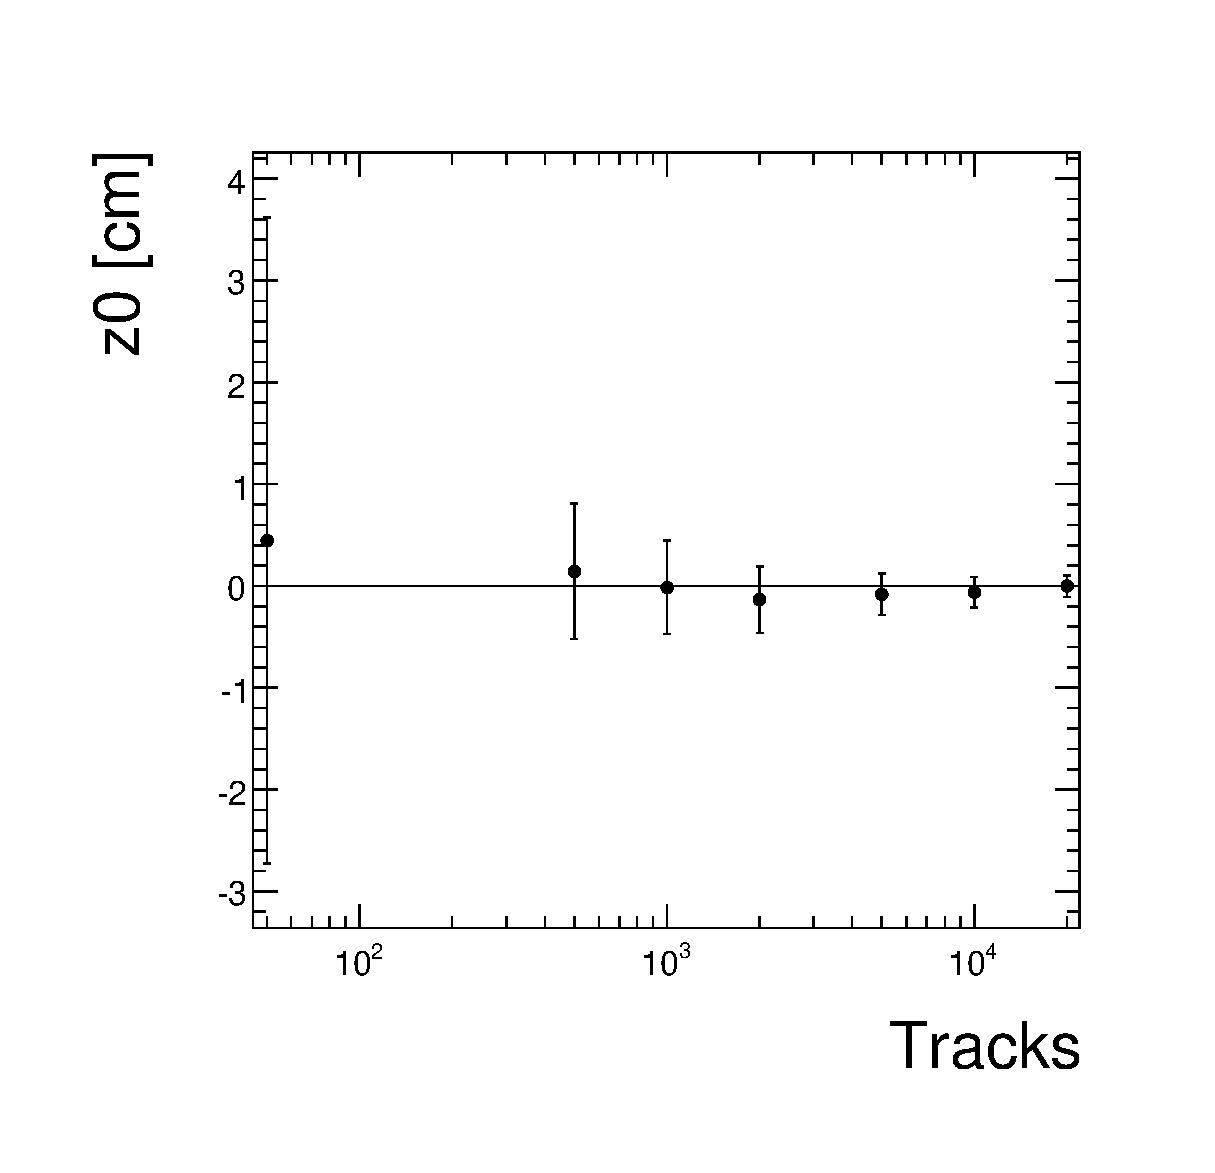
\includegraphics[width=0.45\textwidth]{figures/fxy_lhfit_dz.eps}
        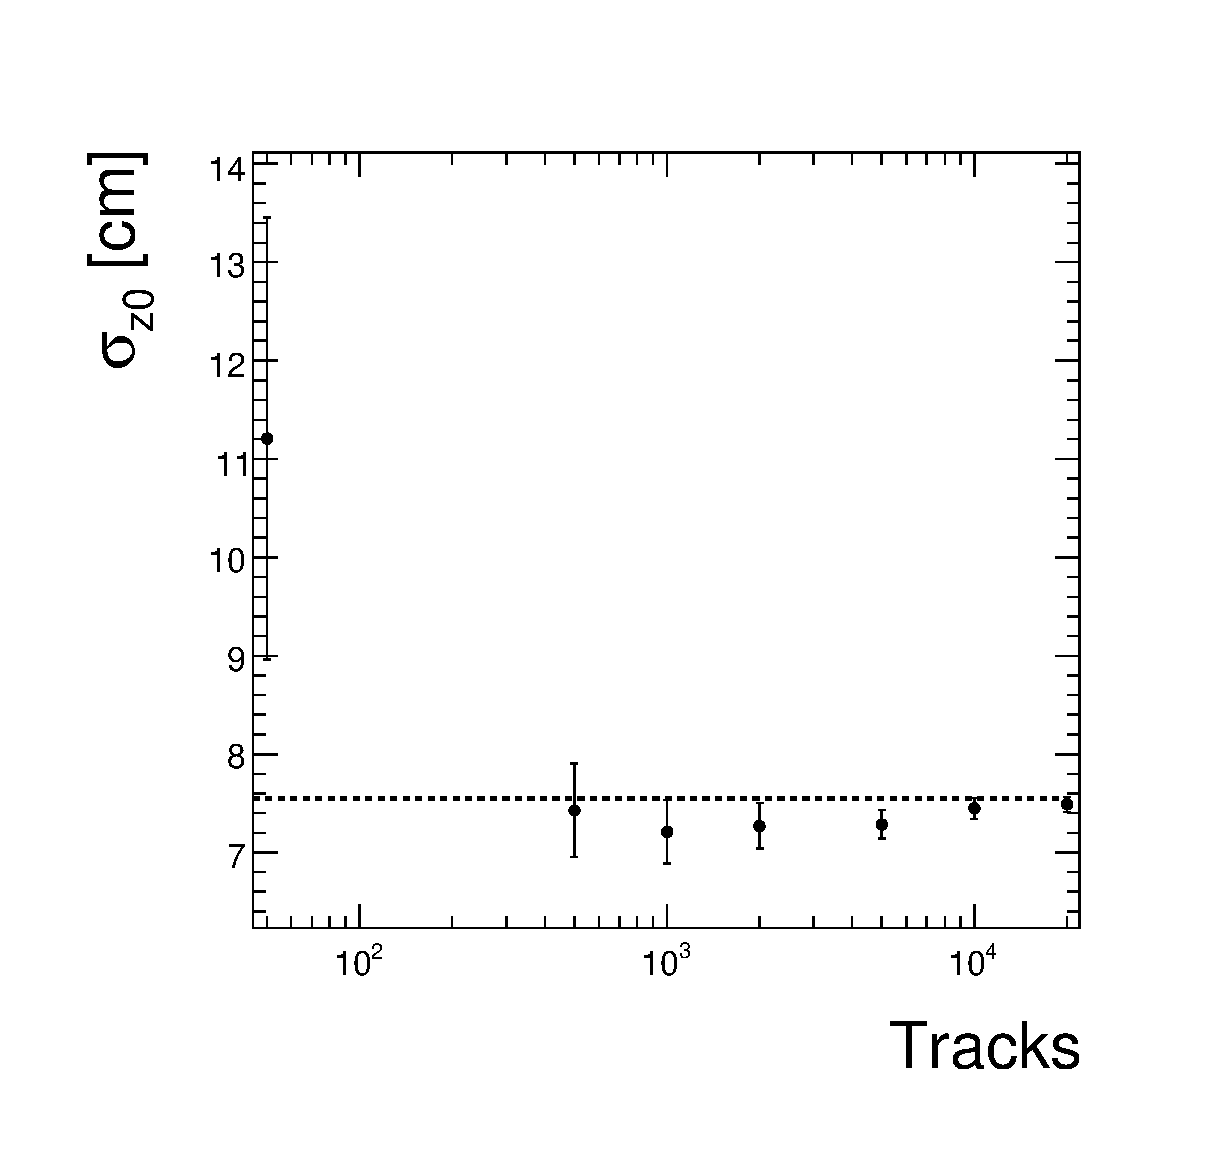
\includegraphics[width=0.45\textwidth]{figures/fxy_lhfit_sigmadz.eps}
        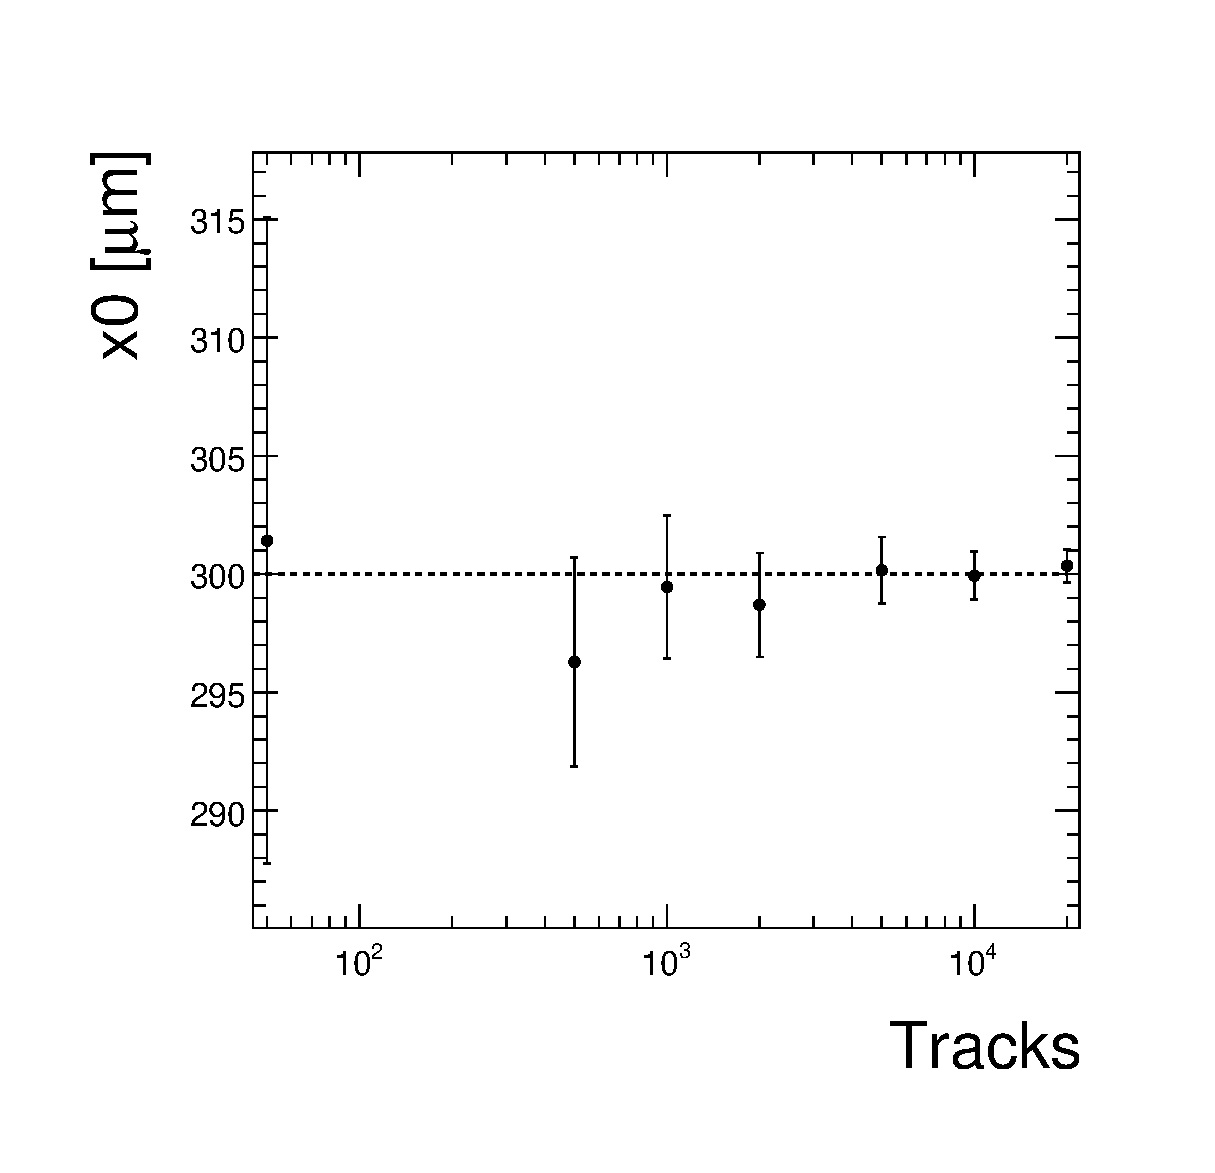
\includegraphics[width=0.45\textwidth]{figures/fxy_lhfit_x0.eps}
        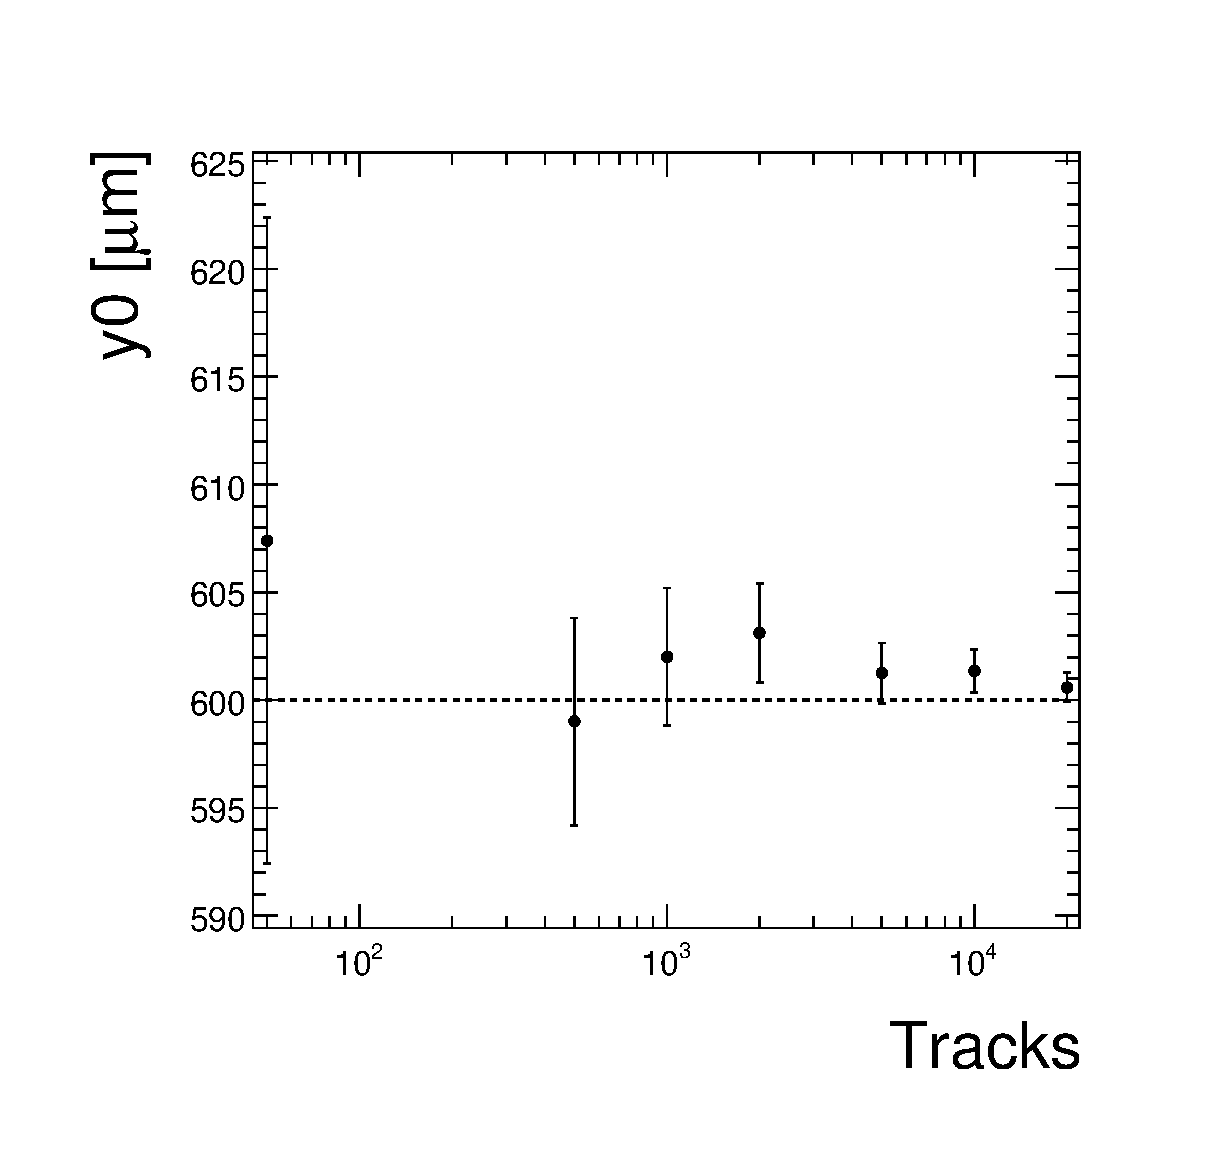
\includegraphics[width=0.45\textwidth]{figures/fxy_lhfit_y0.eps}
        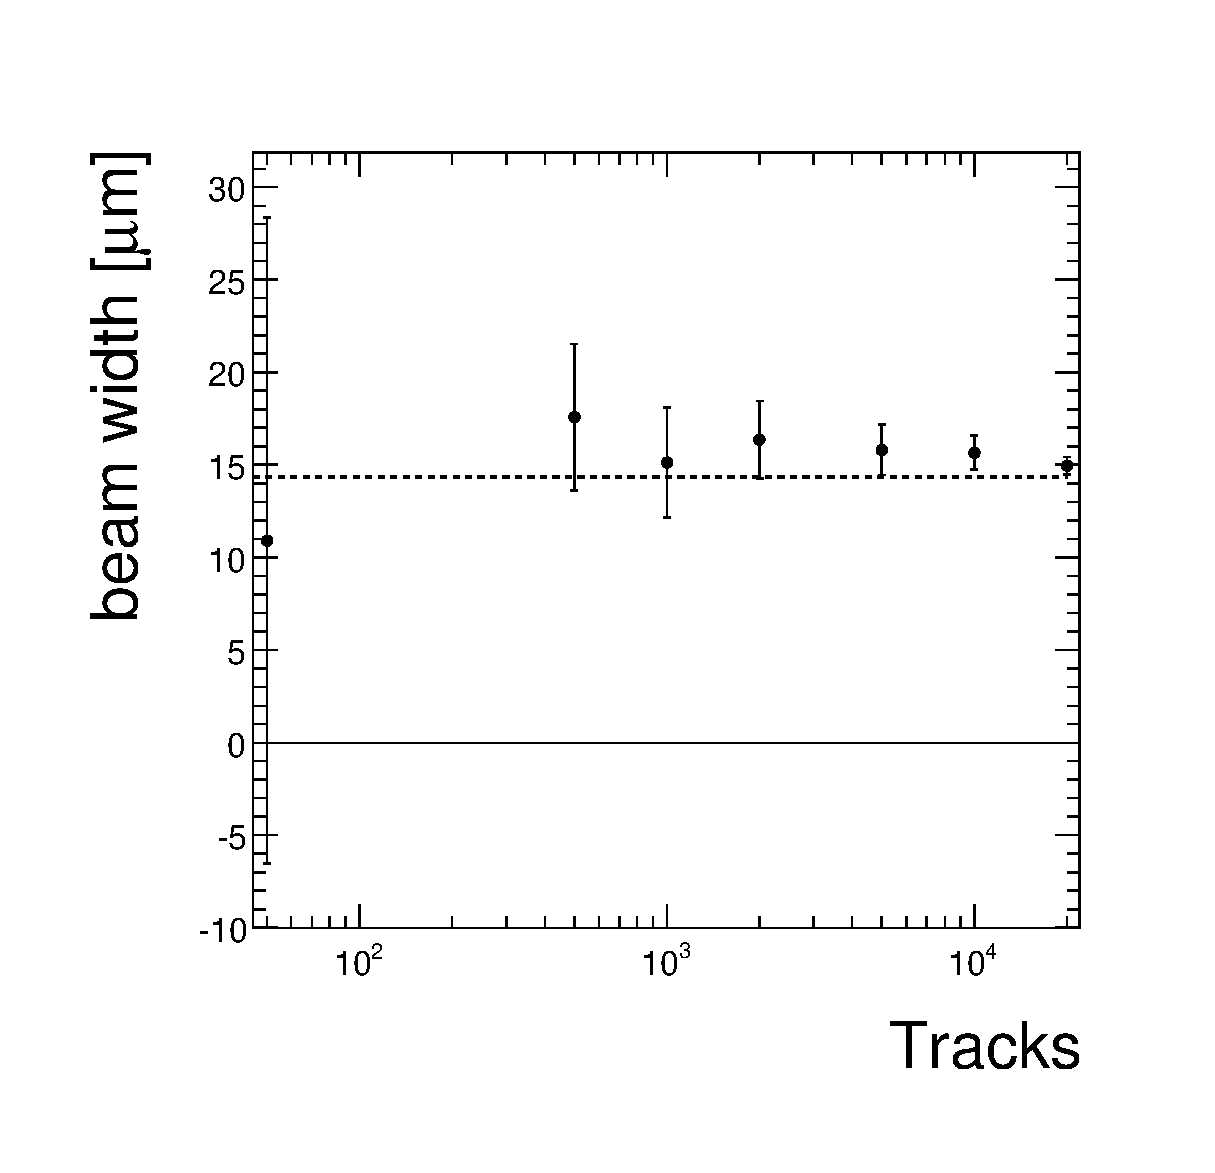
\includegraphics[width=0.45\textwidth]{figures/fxy_lhfit_beamwidth.eps}
%    \resizebox{10cm}{!}{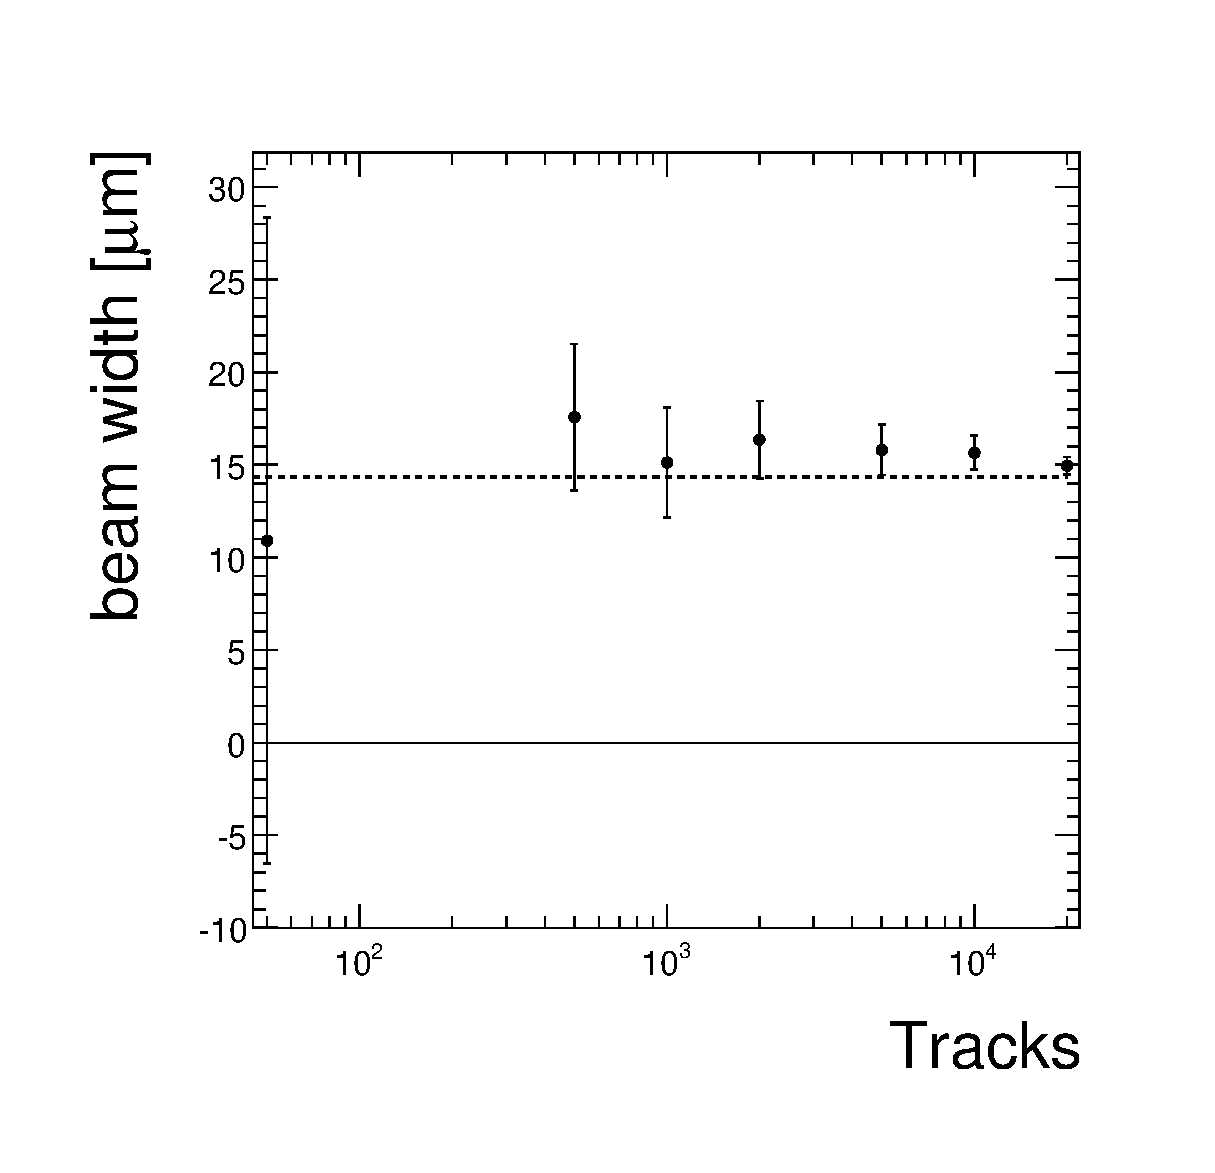
\includegraphics{figures/fxy_lhfit_beamwidth.eps}}
%    \resizebox{10cm}{!}{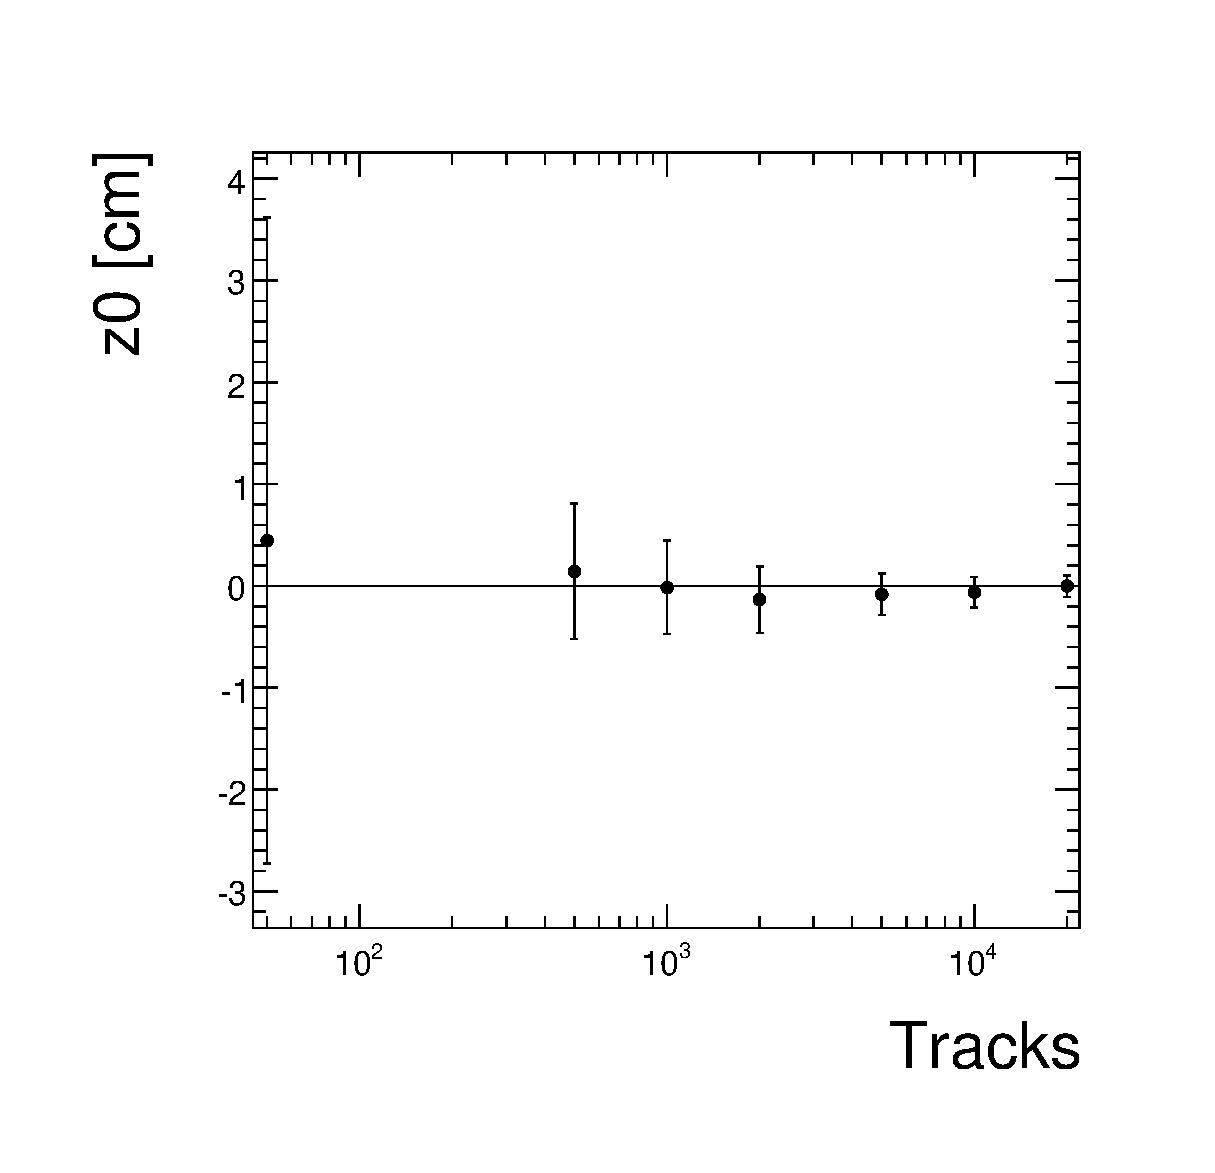
\includegraphics{figures/fxy_lhfit_dz.eps}}
    \caption{\it Convergence of the likelihood fit for: the $z_0$ position and longitudinal width  $\sigma_{z_0}$ of the beam, 
                                                        the transverse $x_0$ and $y_0$ beam position, 
                                                        and the transverse beam width ($\sigma_{Beam}$). 
 This study was done using the fast parametrized Monte 
Carlo simulation with pixels described in Section ~\ref{sec:fast_parameterized_MC}.
                                                         }
    \label{fig:performance_dz}
  \end{center}
\end{figure}

%\begin{figure}[hbtp]
%  \begin{center}
%    \resizebox{10cm}{!}{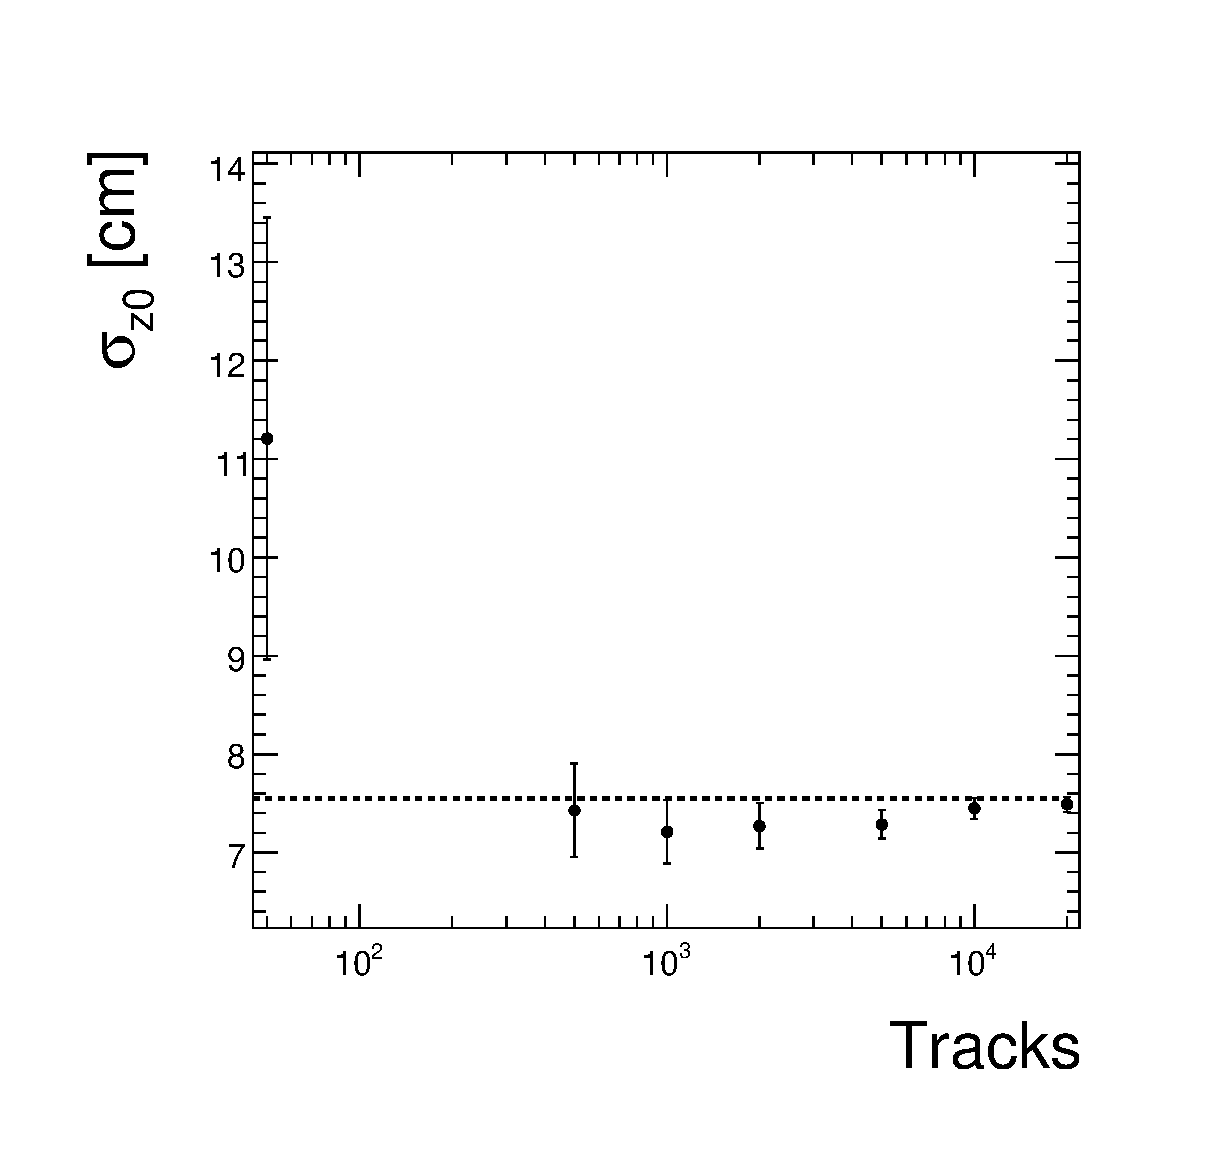
\includegraphics{figures/fxy_lhfit_sigmadz.eps}}
%    \caption{\it Convergence of the likelihood fit for the $\sigma^z$ beam length.}
%    \label{fig:performance_sigmadz}
%  \end{center}
%\end{figure}

%\begin{figure}[hbtp]
%  \begin{center}
%    \resizebox{10cm}{!}{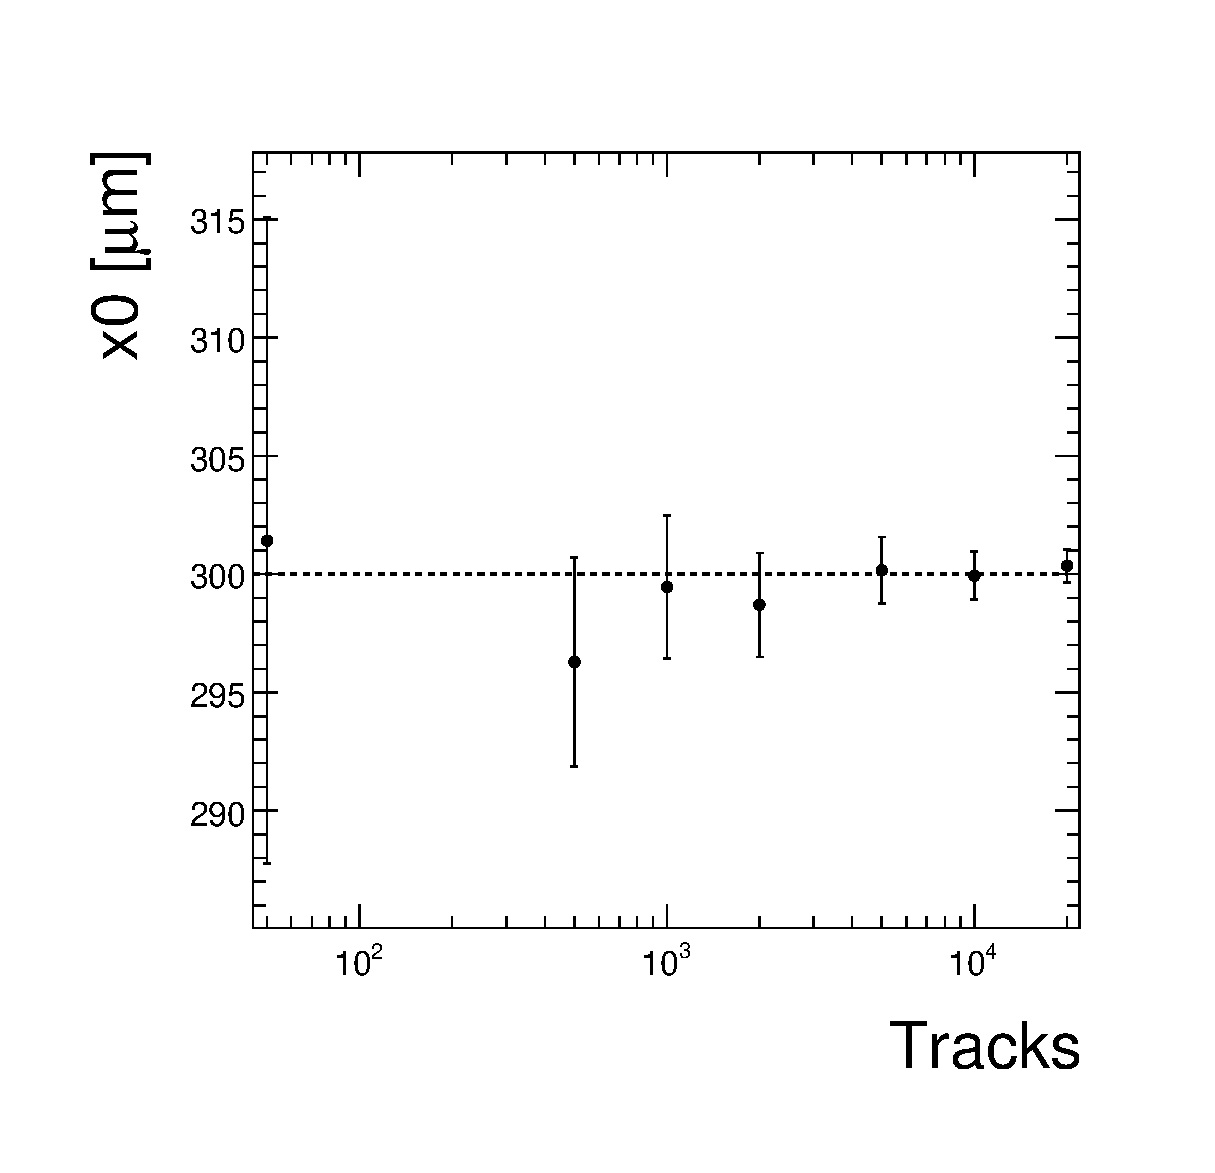
\includegraphics{figures/fxy_lhfit_x0.eps}}
%    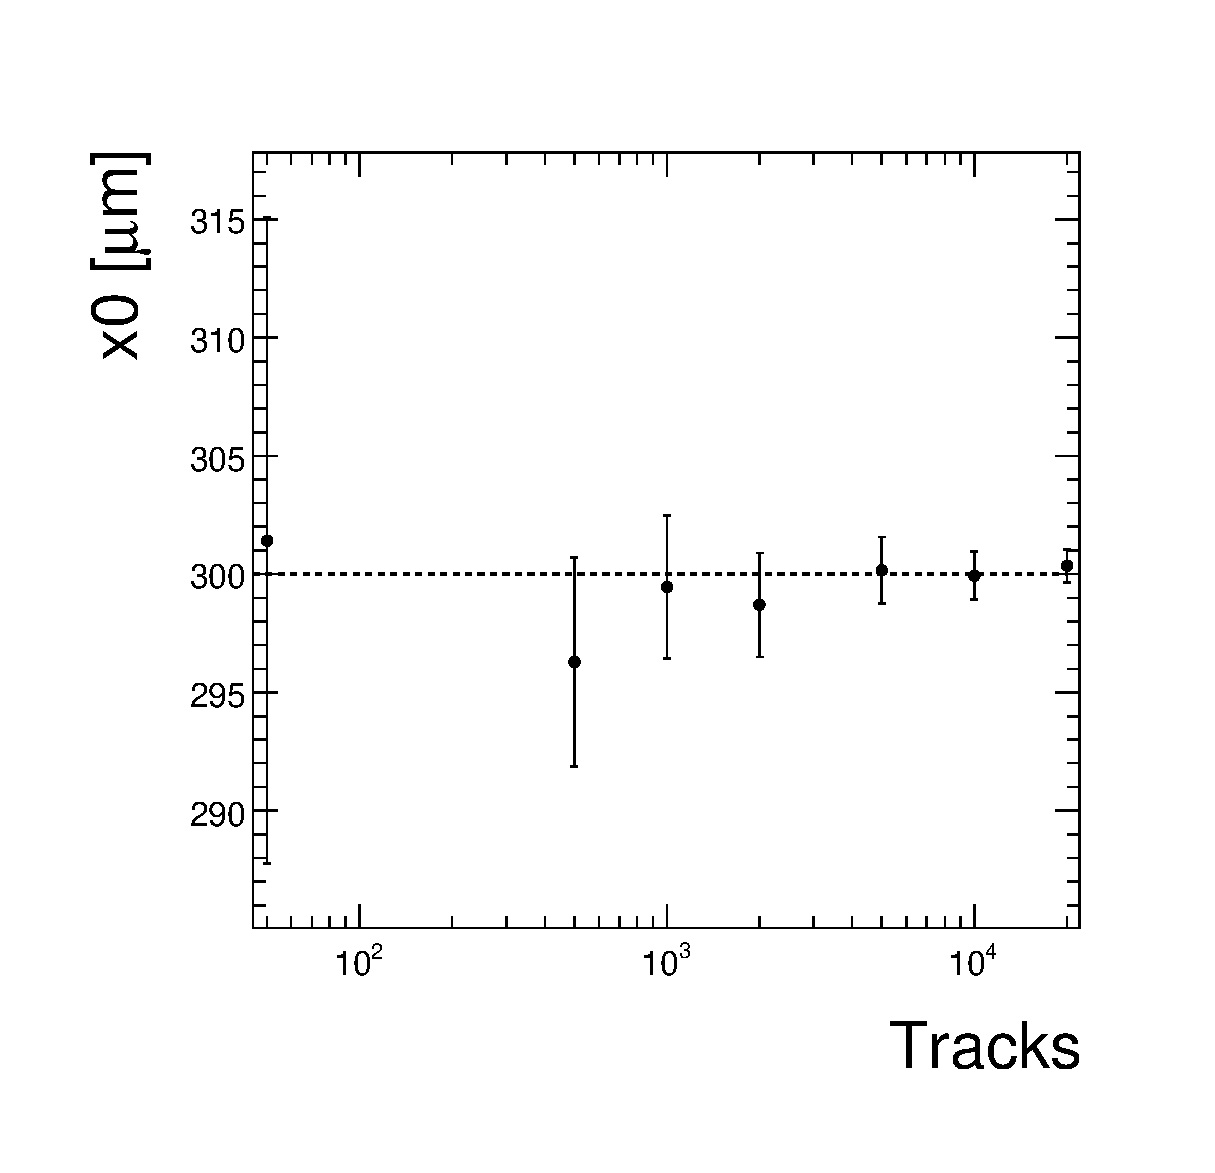
\includegraphics[width=0.45\textwidth]{figures/fxy_lhfit_x0.eps}
%    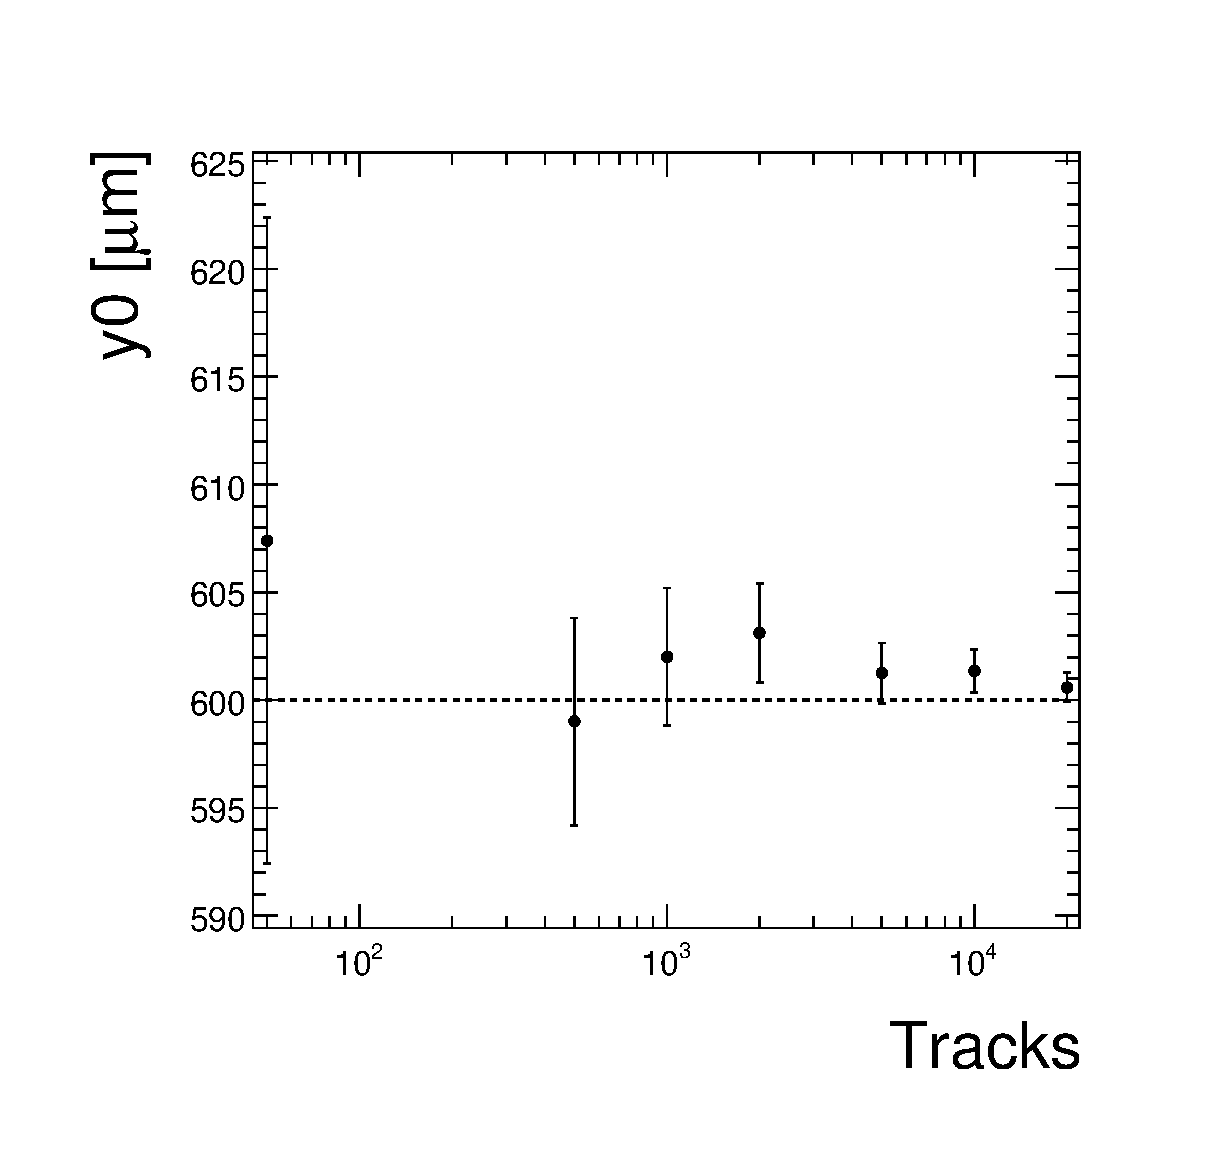
\includegraphics[width=0.45\textwidth]{figures/fxy_lhfit_y0.eps}
%    \caption{\it Convergence of the likelihood fit for the transverse $x_0$ and $y_0$ beam position.}
%    \label{fig:performance_x0}
%  \end{center}
%\end{figure}

%\begin{figure}[hbtp]
%  \begin{center}
%    \resizebox{10cm}{!}{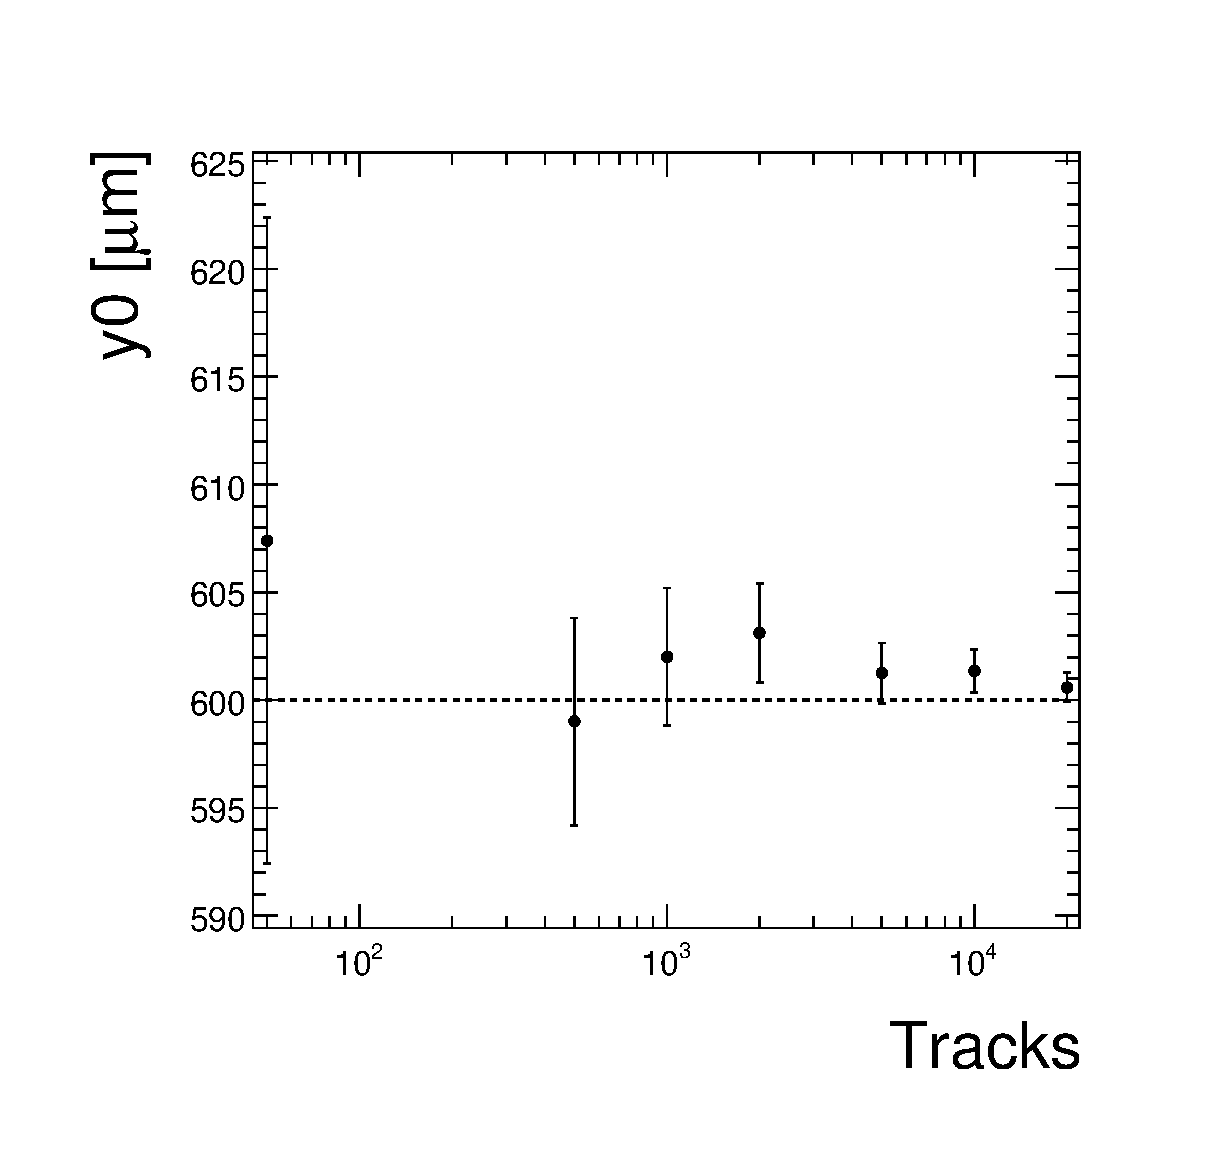
\includegraphics{figures/fxy_lhfit_y0.eps}}
%    \caption{\it Convergence of the likelihood fit for the $y_0$ beam position.}
%    \label{fig:performance_x0}
%  \end{center}
%\end{figure}

%\begin{figure}[hbtp]
%  \begin{center}
%    \resizebox{10cm}{!}{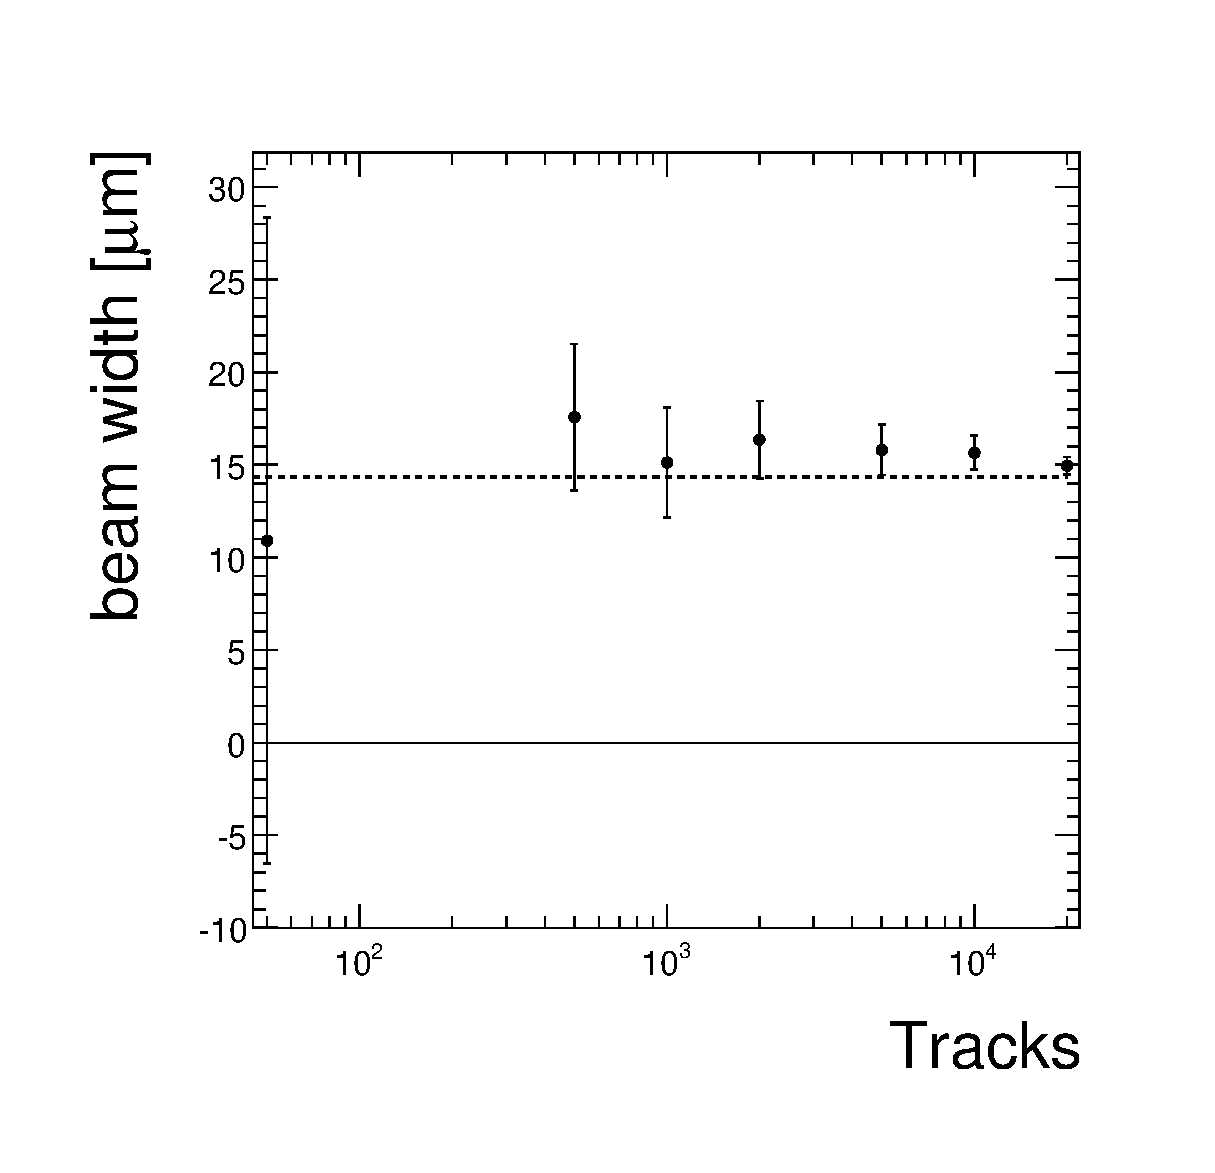
\includegraphics{figures/fxy_lhfit_beamwidth.eps}}
%    \caption{\it Convergence of the likelihood fit for the beam width ($\sigma^{b}$).}
%    \label{fig:performance_beamwidth}
%  \end{center}
%\end{figure}




%\clearpage

\subsection{\label{sec:betafit}Fitting the $\beta$-function}

This fit is the same as the one described in the previous Section \ref{sec:width}, but instead of assuming a constant beam width, 
 the width is allowed to vary with $z$ according to Equation~\ref{betafunction}. Instead of one fit parameter $\sigma_{Beam}$, 
both the emittance $\epsilon$ and $\beta^{*}$ are now fit.
%The CMS detector without pixels does not have sufficient resolution; therefore only results with the pixel system included are given.  
With beam conditions similar to the Tevatron, the CMS tracker with pixel detector would  be able to provide a precise measurement of the beam profile 
in both longitudinal and transverse directions.
Results for various beam scenarios, each based on approximately one million events, are given in Table \ref{BetaFitResult}. 
There are two problems with this fit:
\begin{itemize}
\item  the parameters  $\epsilon$ and $\beta^{*}$ are highly correlated 
       and there is a systematic tendency for the fitted  $\beta^{*}$ to be higher than the input value and the fitted $\epsilon$
       to be lower. This requires a different parameterization of the beam profile, which does not have that problem.
\item  currently no detector acceptance effects are included. These could skew the probability function and would need to be corrected for.  
\end{itemize}
In the nominal LHC scenario the transverse beam width is expected to vary very little over the interaction region justifying the use of
a constant average transverse beam width as described in the previous subsection.     

\begin{table} [th]
\caption{\it \label{BetaFitResult} Beam Profile fitting results for CMS tracker with pixels. All samples consist of 950000 events and 
were generated with nominal $z_0$ at 0.0 cm.}
\begin{center}
\begin{tabular}{|c|c|c|c|c|c|c|} \hline
\multicolumn{3}{|c|}{Input values}& \multicolumn{4}{|c|}{Fitted  values}\\ \hline
$\sigma_z$&$\epsilon$    &$\beta^*$  &   $z_0$&$\sigma_z$ &$\epsilon$   &$\beta^*$\\
$[cm]$    &$[10^{-8}cm]$ &$[cm]$     &$[cm]$  &$[cm]$     &$[10^{-8}cm]$&$[cm]$\\
 \hline      
\hline
 25   & 14   & 35 &$0.006  \pm 0.026$  &$24.70  \pm 0.018$   &$9.96 \pm 0.06$   & $44.37\pm 0.40$
\\ \hline
 11.24& 3.75 & 200&$0.072  \pm 0.012$  &$11.232 \pm 0.0083$  &$2.67  \pm 0.12$    & $227.0\pm 10.3$ 
\\ \hline
 7.55 & 3.75 & 55 &$0.0106 \pm 0.0078$ &$7.55541 \pm 0.0055$  &$3.38  \pm 0.21$    & $68.7\pm 4.5$
\\ \hline
 7.55 & 1.0  & 55 &$0.0048 \pm 0.0078$ &$7.5443  \pm 0.0055$  &$0.97  \pm 0.25$    & $63.8\pm  16.5$
\\\hline
 7.55 & 6.0  & 55 &$  0.048 \pm0.0078$ &$7.543\pm 0.0055$  &$4.69\pm 0.37$    & $63.4\pm  5.2$
\\ \hline
 7.55 & 3.75 & 25 &$0.0048 \pm 0.0078$ &$7.5437  \pm 0.0055$  &$3.49  \pm 0.58$    & $27.57\pm 5.28$
\\\hline
 7.55 & 3.75 & 75 &$0.0048 \pm 0.0078$ & $7.5443  \pm 0.0055$  &$2.83  \pm 0.25$    & $90.86\pm 8.02$
\\ \hline 
\end{tabular}
\end{center}

\end{table}

\begin{figure}[hbtp]
  \begin{center}
    \resizebox{7cm}{!}{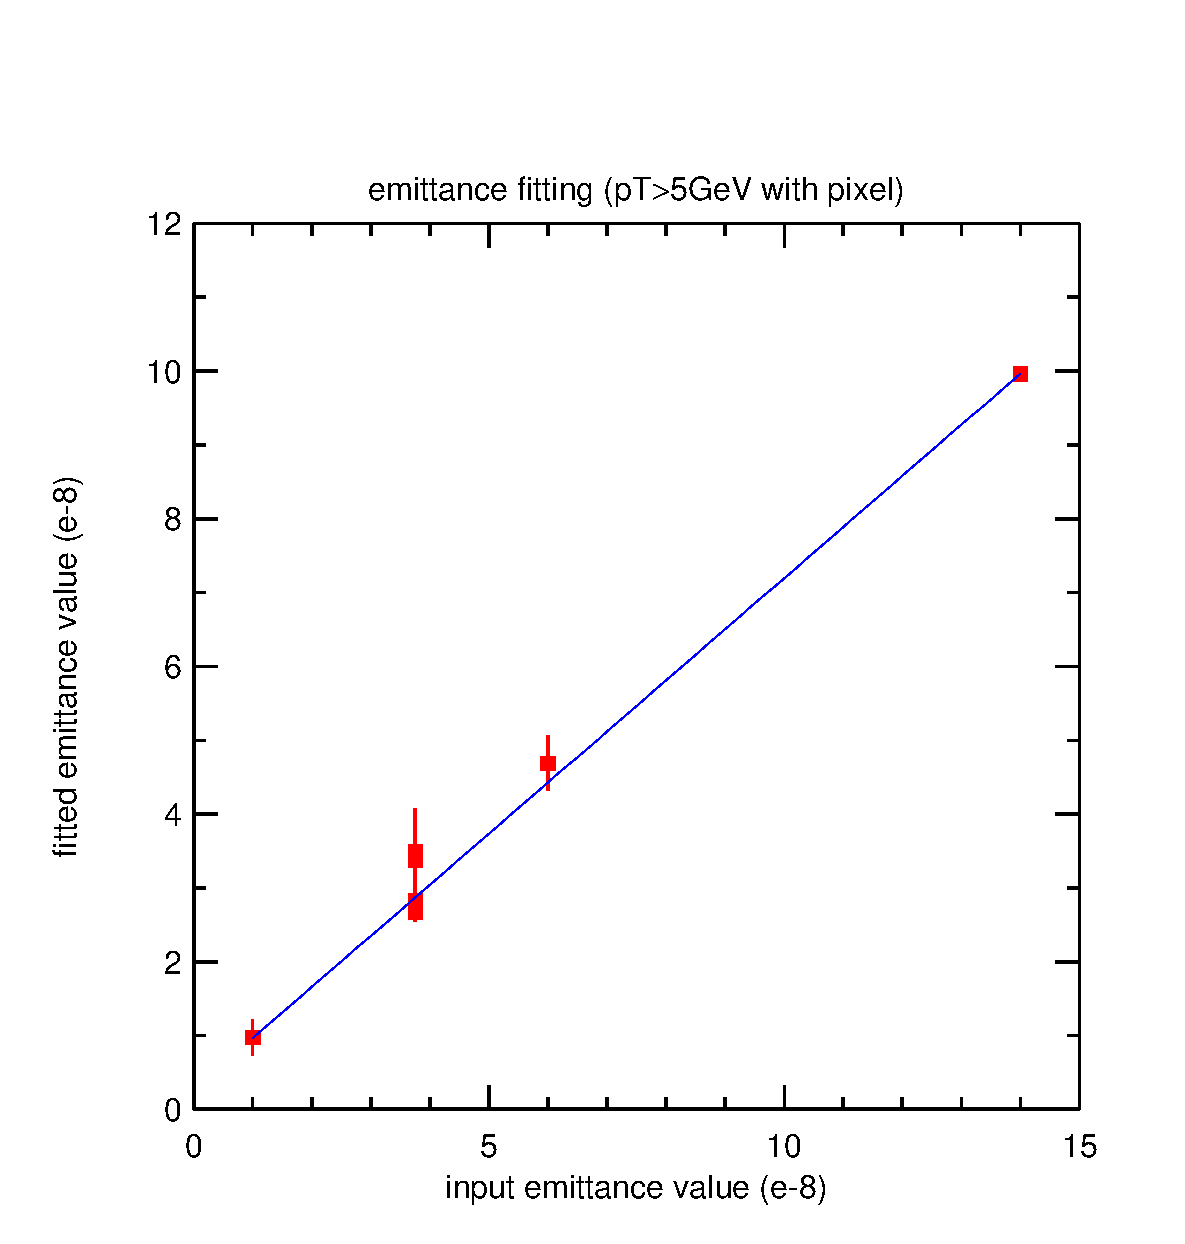
\includegraphics{figures/emittance_fit_line.eps}}
    \resizebox{7cm}{!}{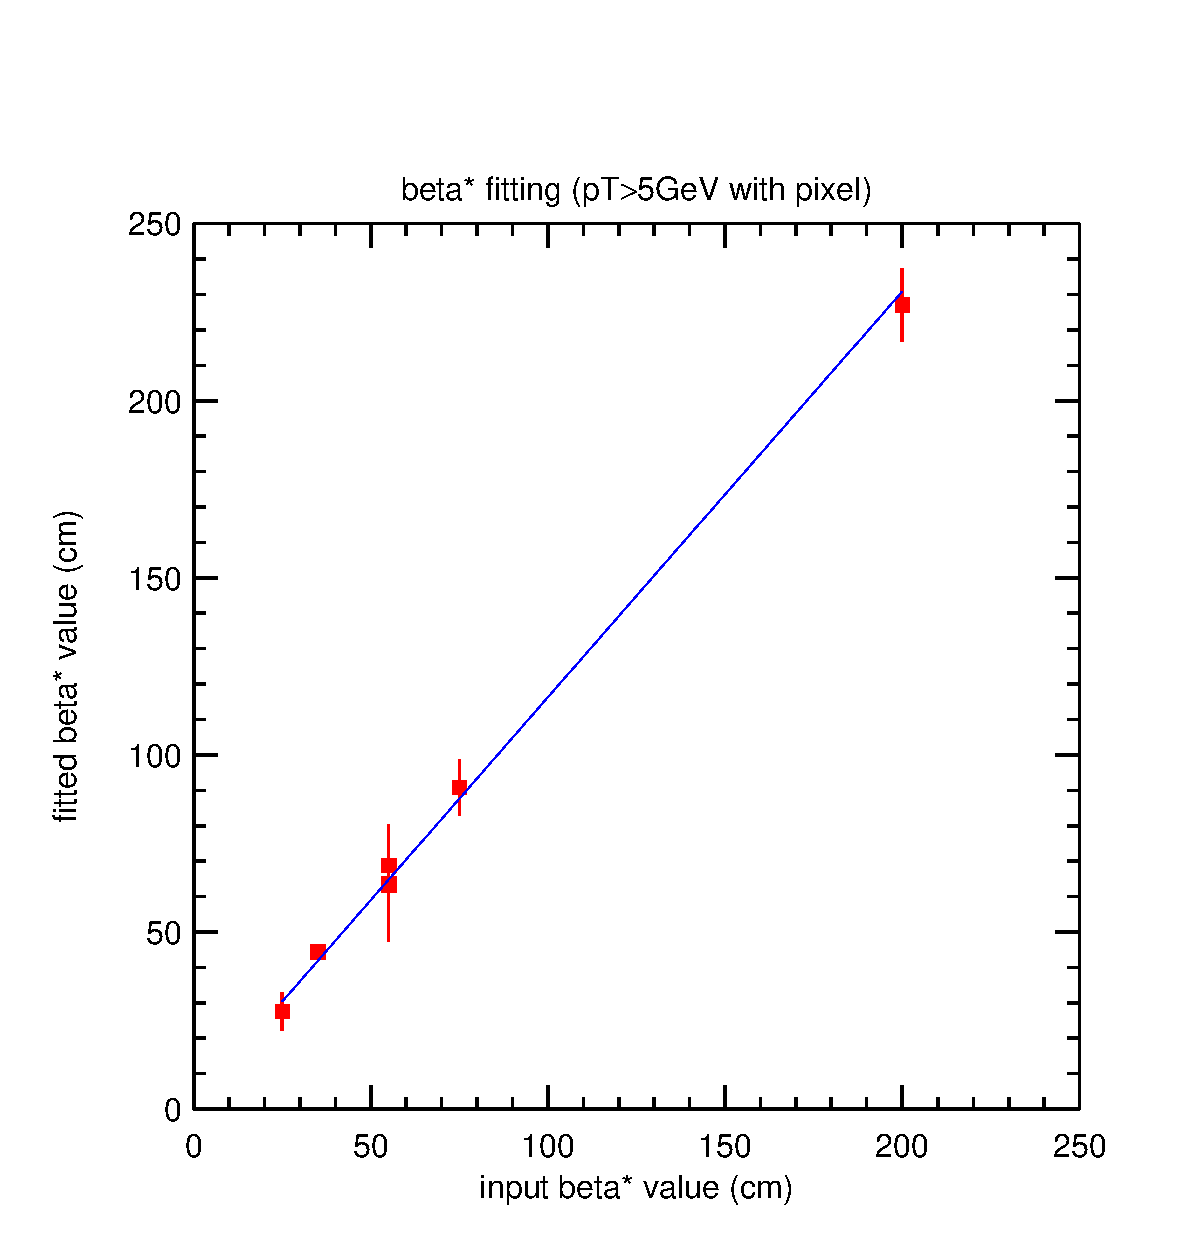
\includegraphics{figures/beta_fit_line.eps}}
    \caption{\it Beam profile fit result with pixel in CMS. This study was done using the fast parametrized Monte 
Carlo simulation described in Section ~\ref{sec:fast_parameterized_MC}.}
    \label{fig:beamprofile}
  \end{center}
\end{figure}




%\subsection{\label{sec:cmsswimp}Implementation of {fitters} in \texttt{CMSSW}}

%The $d_0 - \varphi_0$ and log-likelihood fits have been implemented in a \texttt{CMSSW} package called BeamSpotProducer
%~\cite{BeamSpotProducer}. This package also includes a class object (BeamSpot) that holds all the beam information: 
%XYZ beam position, two slopes, RMS beam length, beam width, and a full covariance matrix. This
%object can be used to store the beam information in the database.

%The fitters take as input a vector of tracks and then apply the fits selected by the user. The fits
%available are: $\chi^2$ and log-likelihood fits for $z$-distribution,
%$d_0 - \varphi_0$ fitter, log-likelihood fit for beam position and  
%log-likelihood fit for extraction of the beam width. The likelihood fitters have been implemented
%using MINUIT2, a C++ version of the well known MINUIT package.

%Table~\ref{d0phiresultsfullsim} shows the results of the $d_0-\varphi_0$ fitter over different
%fully GEANT 4 simulated and reconstructed samples.


\clearpage
\section{\label{sec:ipextract}Extracting the average Impact Parameter resolution function}
%Once  the beam position and beam width are measured with high precision using the methods described in the previous Section or by other means, 
%this information can be used to study some aspects of the tracking performance.
The expected width of the LHC beam in the CMS interaction region is  $16$ $\mu$m and can be considered constant in $z$. 
This is smaller than the expected single track resolution even with the pixel system. 
This fact can be used to directly measure and monitor the average single track impact parameter resolution of the 
Tracker. The width of the impact parameter distribution with respect to the beam has two contributions:
the width of the beam and the  impact parameter resolution of the tracking detector. These two contributions behave very 
differently. While the beam width is constant, the impact parameter resolution is a function of the transverse momentum 
of the track. This fact helps to disentangle the two. 
%This will be especially important during the commissioning phase allowing us to validate the alignment, to check that the 
%material in the detector is modeled correctly and to check that the calculated IP uncertainty returned from the fit is correct. 
In this Section, two studies are presented.  The first study, based on the fast Monte Carlo simulation, uses the 
Log-likelihood fitter to extract the parameters of the impact parameter resolution function. 
The second study is based on the full simulation and  reconstruction.
In this study, the  impact parameter and pull distributions for different bins in $p_T$ are fitted to extract the impact 
parameter resolution function and to check the impact parameter uncertainty returned by the track fit. 
For both studies, the position and slope of the beam are first determined with high precision using the  
$d_0-\varphi_0$ fitter. Then the track parameters are recalculated with the fitted beam 
as a new reference point. The uncertainty of beam position and slope given by the $d_0-\varphi_0$ fit is small and 
can be neglected.  

 
\subsection{\label{sec:ipresol}The Log-likelihood {fitter} to extract the Impact Parameter Resolution}

%In this subsection we introduce a  Log-likelihood fitter to extract the IP resolution and study the performance of the 
%fitter with the fast Monte Carlo simulation. 

Once all the beam parameters (position, slope and width) are well known they can be fixed, in the likelihood function 
described by 
Eq. (\ref{eq:likelihood}), while the parameters $c_0$ and  $c_1$ of the impact parameter resolution function 
Eq. (\ref{ptpara}) are allowed to vary. The values  of $c_0$ and $c_1$ can then be extracted
minimizing the likelihood function Eq. (\ref{eq:likelihood}).

Using the fast parametrized Monte 
Carlo simulation, samples with different impact parameter resolutions were produced. 
The two impact Parameter resolution scenarios used to smear the generated tracks are:
\begin{enumerate}
\item $\sigma^{tr}_{d0}(p_T) =10 + 90/p_T$ [$\mu$m] (as expected with pixels from full GEANT 4 simulation).
\item $\sigma^{tr}_{d0}(p_T) =100 + 900/p_T$ [$\mu$m] (as expected without pixels  from full GEANT 4 simulation).
\end{enumerate}


%The 90\% confidence limits for the transverse position of the beam are shown in 
%Figure~\ref{fig:contours}(a). The marker shows the input value used to generate the samples. For
%scenario (1), 20k tracks are used in the fit while 50k tracks and tightend $p_T$ 
%selection are required in scene ray (2). As the resolution gets worse, the errors on the
%transverse beam position increase however an average position can still be measured.
%In Figure~\ref{fig:contours}(b), the results of the beam width calculation are shown for the
%two different IP resolution scenarios.  For the beam width calculation, the errors increase much more and the width cannot be resolved
%for scenario (2). For the case of a detector without pixels, where the resolution
%is $\sigma_{d0}=100+900/p_T$ [$\mu$m], it will not be possible to estimate the beam width with
%this technique.


% francisco   
%\begin{figure}[hbtp]
%  \begin{center}
%    \resizebox{10cm}{!}{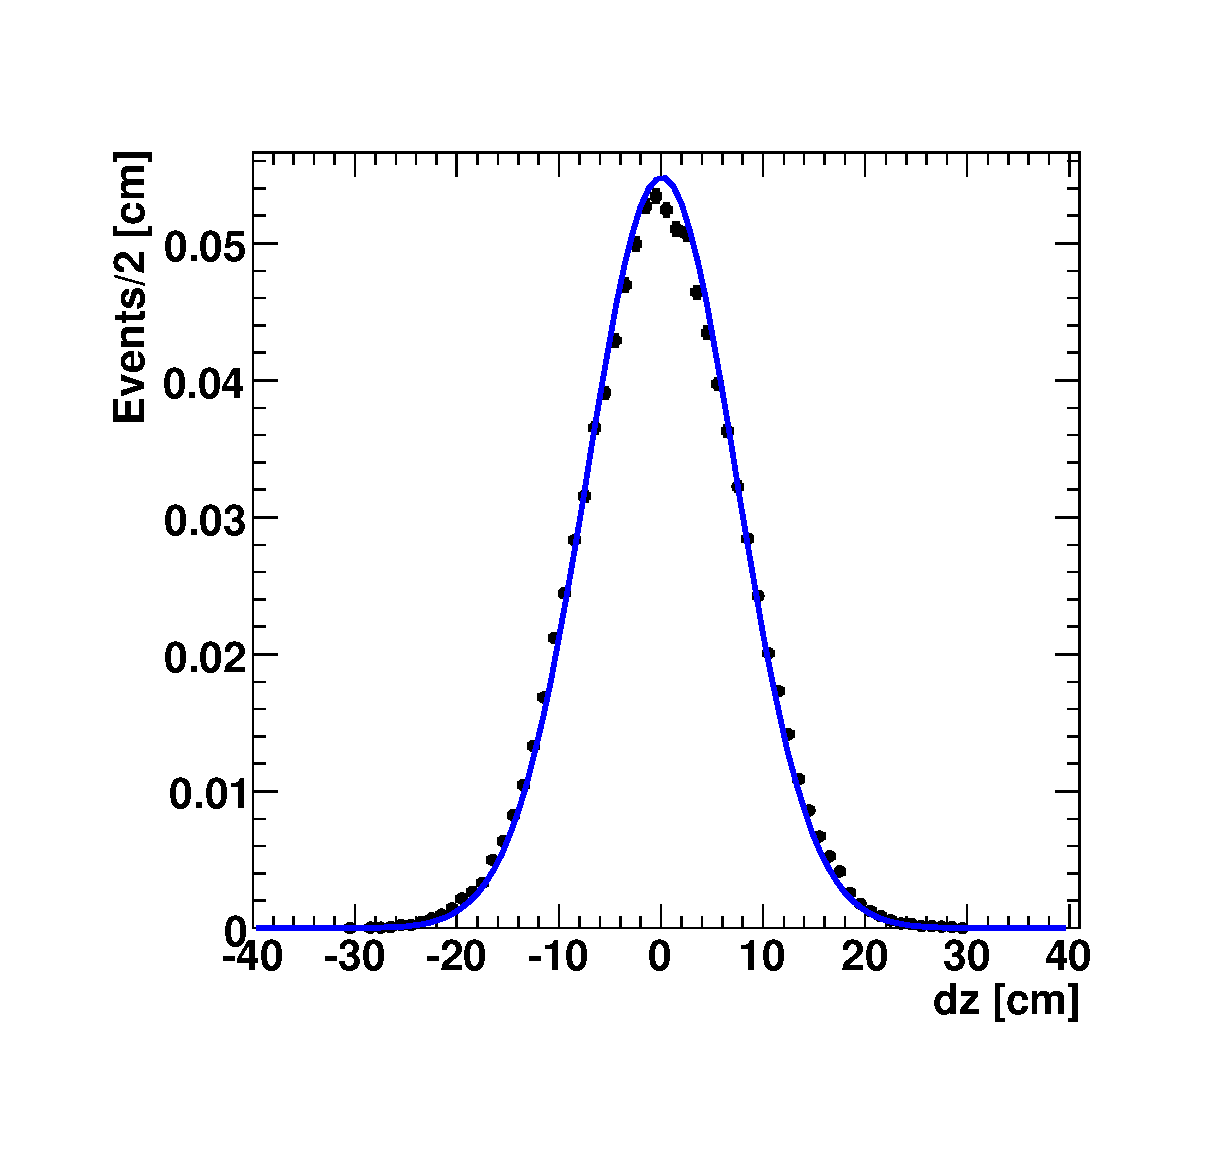
\includegraphics{figures/fxy_gaussfit_dz.eps}}
%    \caption{\it Impact parameter distribution along the longitudinal axis. The simulated 
%    data is shown as black markers and the result of the likelihood fit as a solid line.}

%    \label{fig:gaussfit_dz}
%  \end{center}
%\end{figure}

%\section{Performance of the fitters} 
%Here we write about the performance of the different fitters. Performance parameters include:
%speed, convergence behavior, how much data is needed, robustness, behavior of covariance matrix 
%etc. 

%The fit procedure is the following: first, the $d_0 - \varphi_0$ fitter is run to extract the initial values, 
%then the  log-likelihood fit is run to extract the beam width, and finally the former fit is computed again 
%with a fixed beam width. In this exercise, the beam width has been chosen to be the generated value. 

 
The convergence of the likelihood fit for the $c_0$ and  $c_1$ impact parameter resolution parameters are shown in Figure \ref{fig:performance}
for the scenario with pixels. 
The dotted lines represent the input value used to generate the sample. The case for a detector without pixels is shown
in Figure~\ref{fig:performance2}. 

\begin{figure}[hbtp]
  \begin{center}
    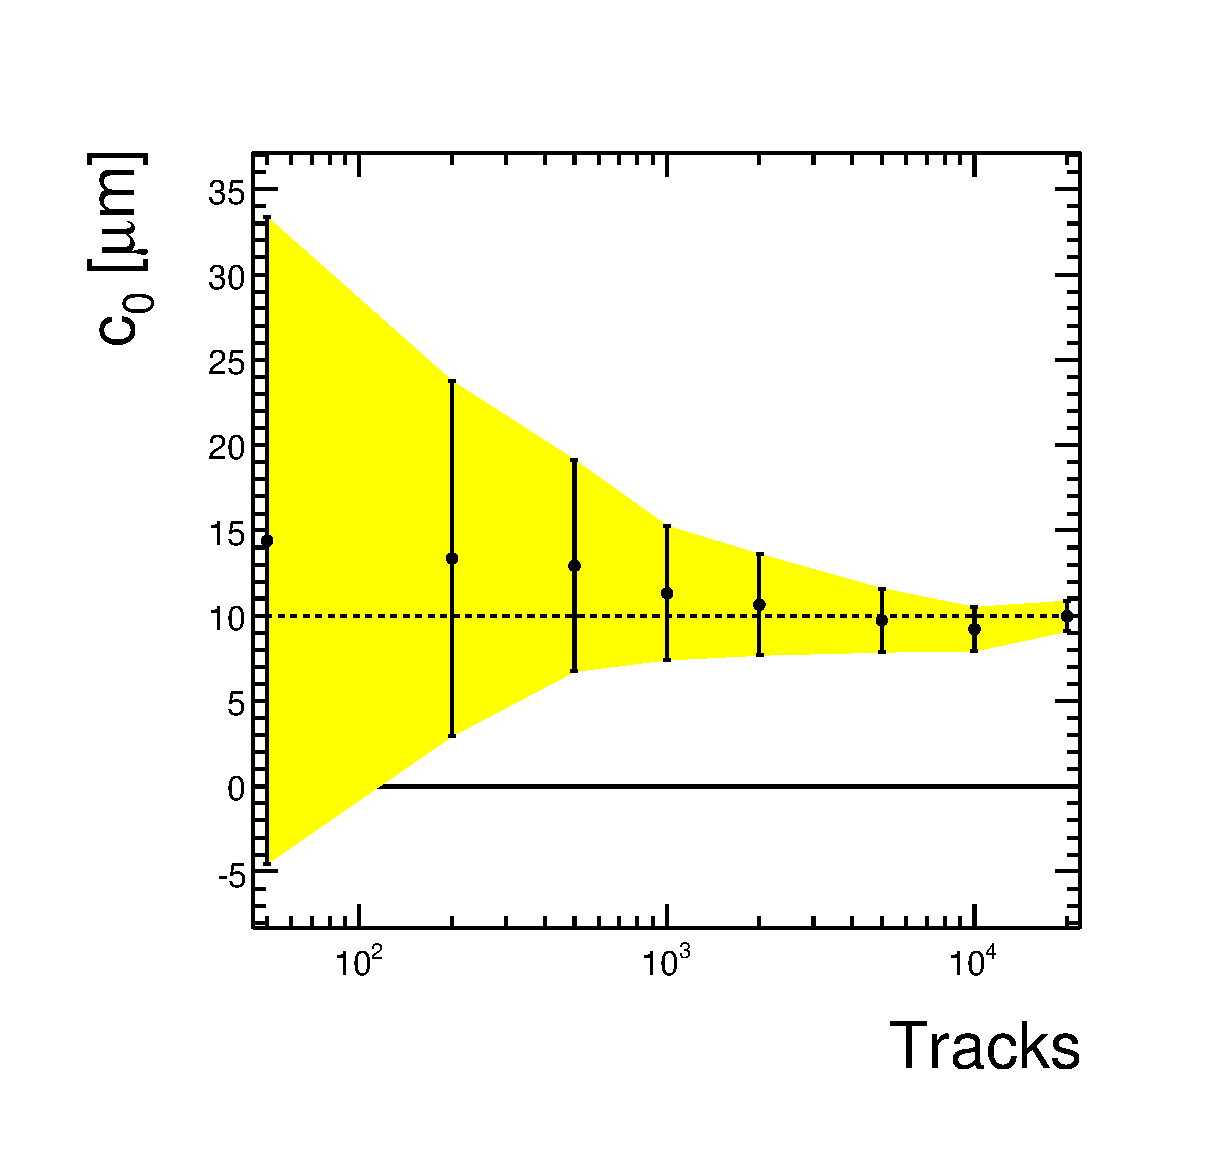
\includegraphics[width=0.45\textwidth]{figures/fxy_lhfit_c0.eps}
    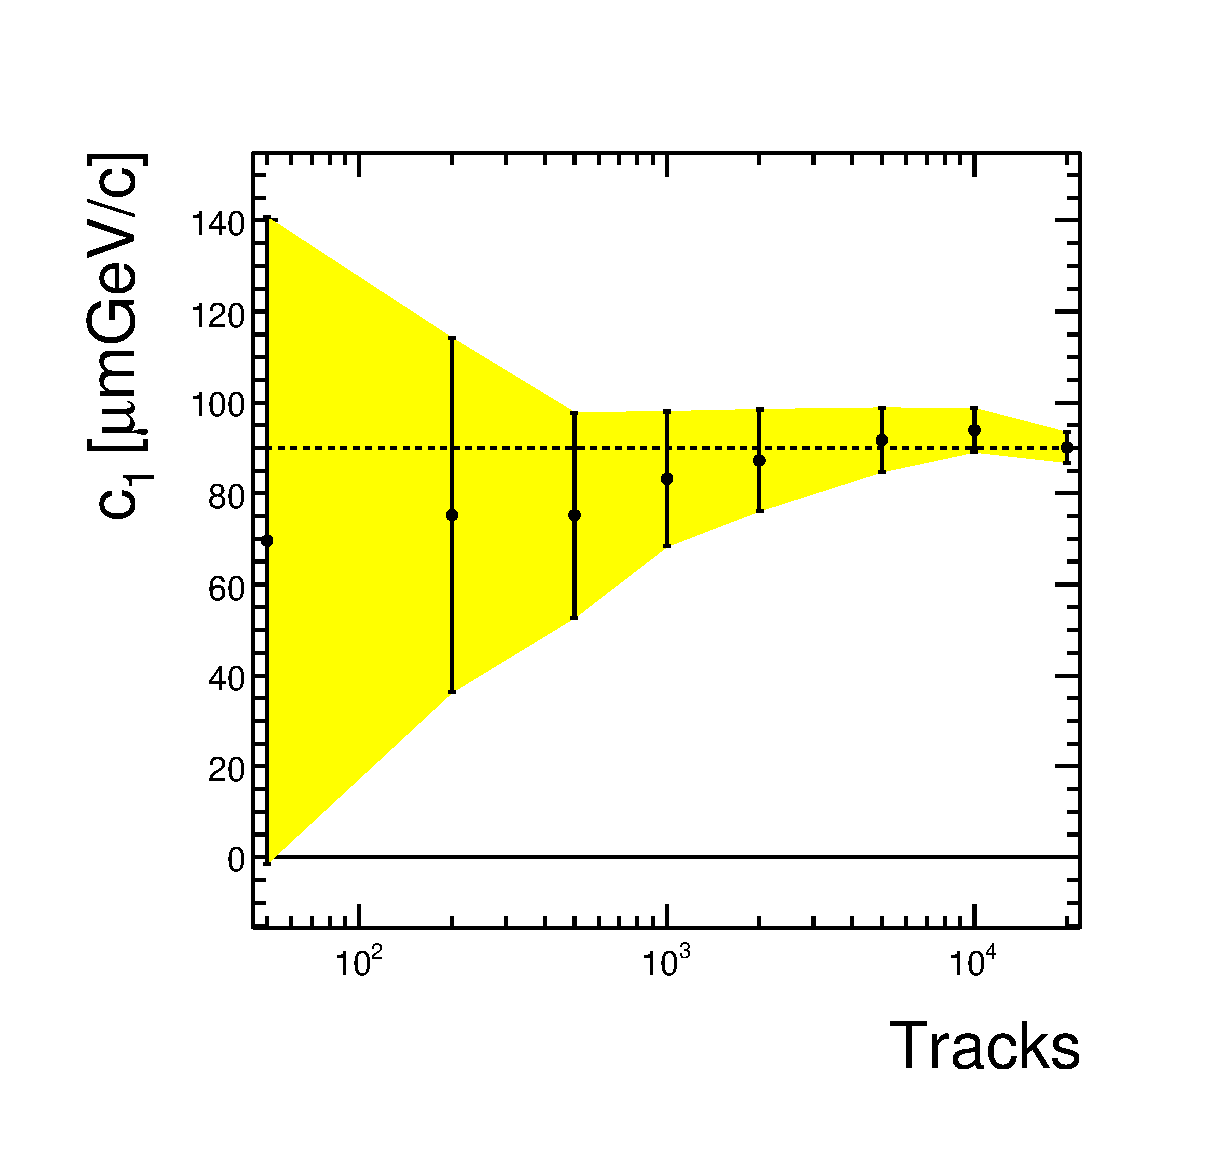
\includegraphics[width=0.45\textwidth]{figures/fxy_lhfit_c1.eps}
   \caption{\it Convergence of the likelihood fit for the $c_0$ and  $c_1$ impact parameter resolution parameters, for impact parameter resolution 
scenario (1). This study was done using the fast parametrized Monte 
Carlo simulation with pixels described in Section ~\ref{sec:fast_parameterized_MC}.}
   \label{fig:performance}
  \end{center}
\end{figure}

\begin{figure}[hbtp]
  \begin{center}
    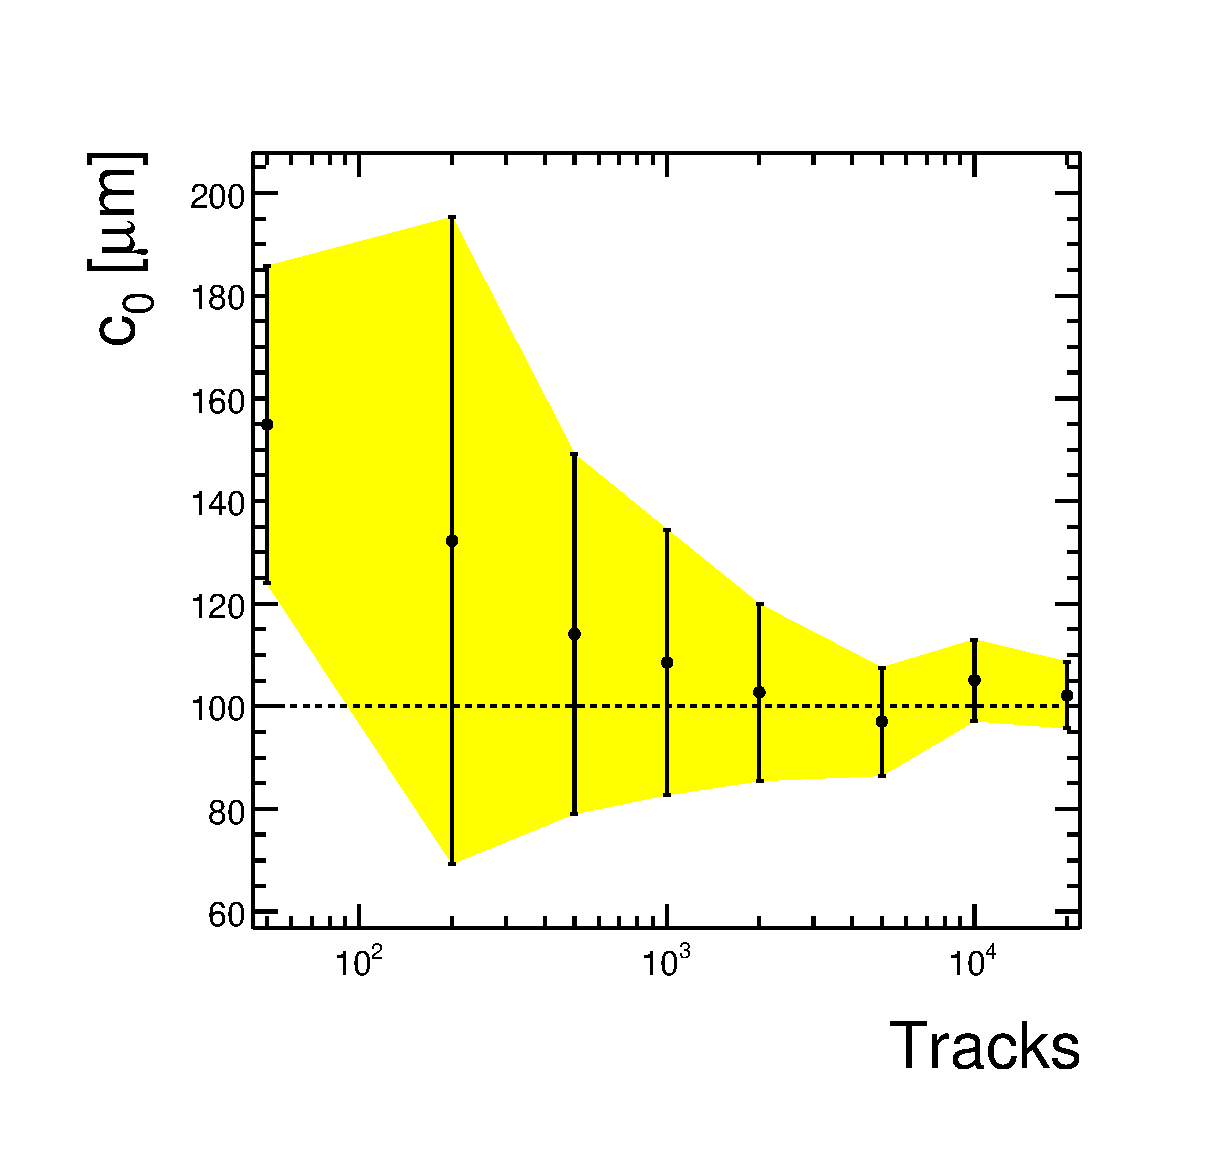
\includegraphics[width=0.45\textwidth]{figures/fxy_lhfit_c0_scen2.eps}
    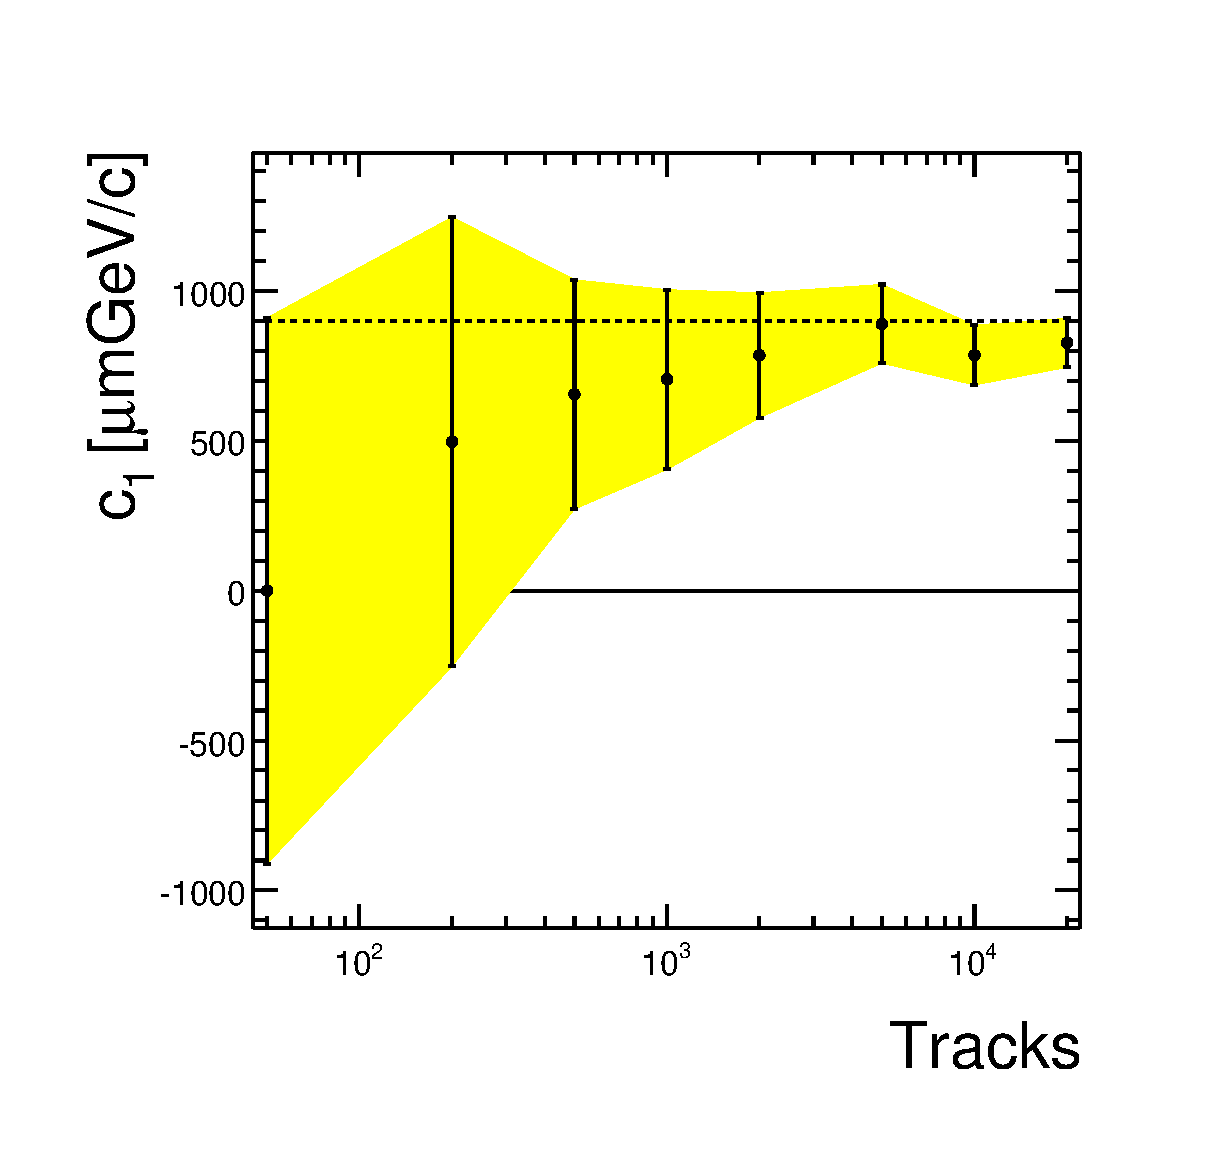
\includegraphics[width=0.45\textwidth]{figures/fxy_lhfit_c1_scen2.eps}
   \caption{\it Convergence of the likelihood fit for the $c_0$ and  $c_1$ impact parameter resolution parameters, for impact parameter resolution 
scenario (2). This study was done using the fast parametrized Monte 
Carlo simulation with pixels described in Section ~\ref{sec:fast_parameterized_MC}.}
   \label{fig:performance2}
  \end{center}
\end{figure}



\clearpage

\subsection{\label{sec:ipresolfull}Measurement of the average Impact Parameter resolution from the full Monte Carlo simulation}


   
All the results in this subsection are obtained using the full Monte Carlo simulation with pixels described in Section \ref{sec:full_MC}.
First, the impact parameter $d'_{0}$ (Eq.~\ref{eq:dprime0}) is calculated in the beam reference frame  and plotted for different $p_T$ bins as shown in  
Figure ~\ref{fig:d0prime_array}. 
The distributions get narrower for higher $p_T$ values as the contribution from multiple scattering decreases with $p_T$.
These distributions are fitted to a Gaussian distribution function. The fact that the impact parameter resolution varies with
the polar angle, as the track traverses more material, is not taken into account and the distributions are only approximately  
described by a Gaussian function. 
We use the $\sigma$ of the Gaussian as an approximation of the impact parameter resolution averaged over all polar angles. 
As described in Equation ~\ref{eq:sigmadprime0}, two components contribute to the width of this
distribution, the transverse width of the beam, $\sigma_{Beam}=16$~$\mu$m, and the impact parameter resolution of the tracker. 
%$\left(\sigma_{Distribution}(p_T)\right)^2 = \left(\sigma^{tr}_{d0}(p_T)\right)^2+\sigma_{Beam}^2$,
%from which 
So once the width of the beam is known one can extract the impact parameter resolution 
of the tracker: 
$\sigma^{tr}_{d0}(p_T) = \sqrt{(\sigma_{Distribution}(p_T))^2 -\sigma_{Beam}^2}$.
This is plotted in  Figure ~\ref{fig:reso_d0prime_fit}.
The parameters of the resolution function are obtained by fitting this distribution with a linear function. 
The result of the fit is given on the same plot.
 
The normalized pull distributions  $\frac{d'_{0}}{ \sqrt{(\sigma^{tr}_{d0}(p_T))^2 +\sigma_{Beam}^2}}$ are  shown in Figure \ref{fig:normd0prime}.
These distributions are expected to be well described by a Gaussian distribution with a mean of 0 and a standard deviation $\sigma$ of 1 and serve 
as a test that the impact parameter resolution as determined by the track fit is correct. Compared to the distributions  in Figure ~\ref{fig:d0prime_array}
the normalized distributions should really be Gaussian since the impact parameter uncertainty returned by the track fit should include all effect like the polar
angle dependence.  In this case, the errors returned by the fit seem to be underestimated by 
10 to 20\% depending on track $p_T$ (see Figure ~\ref{fig:norm_d0prime_fit}).   


\begin{figure}[htp]
  \centering
    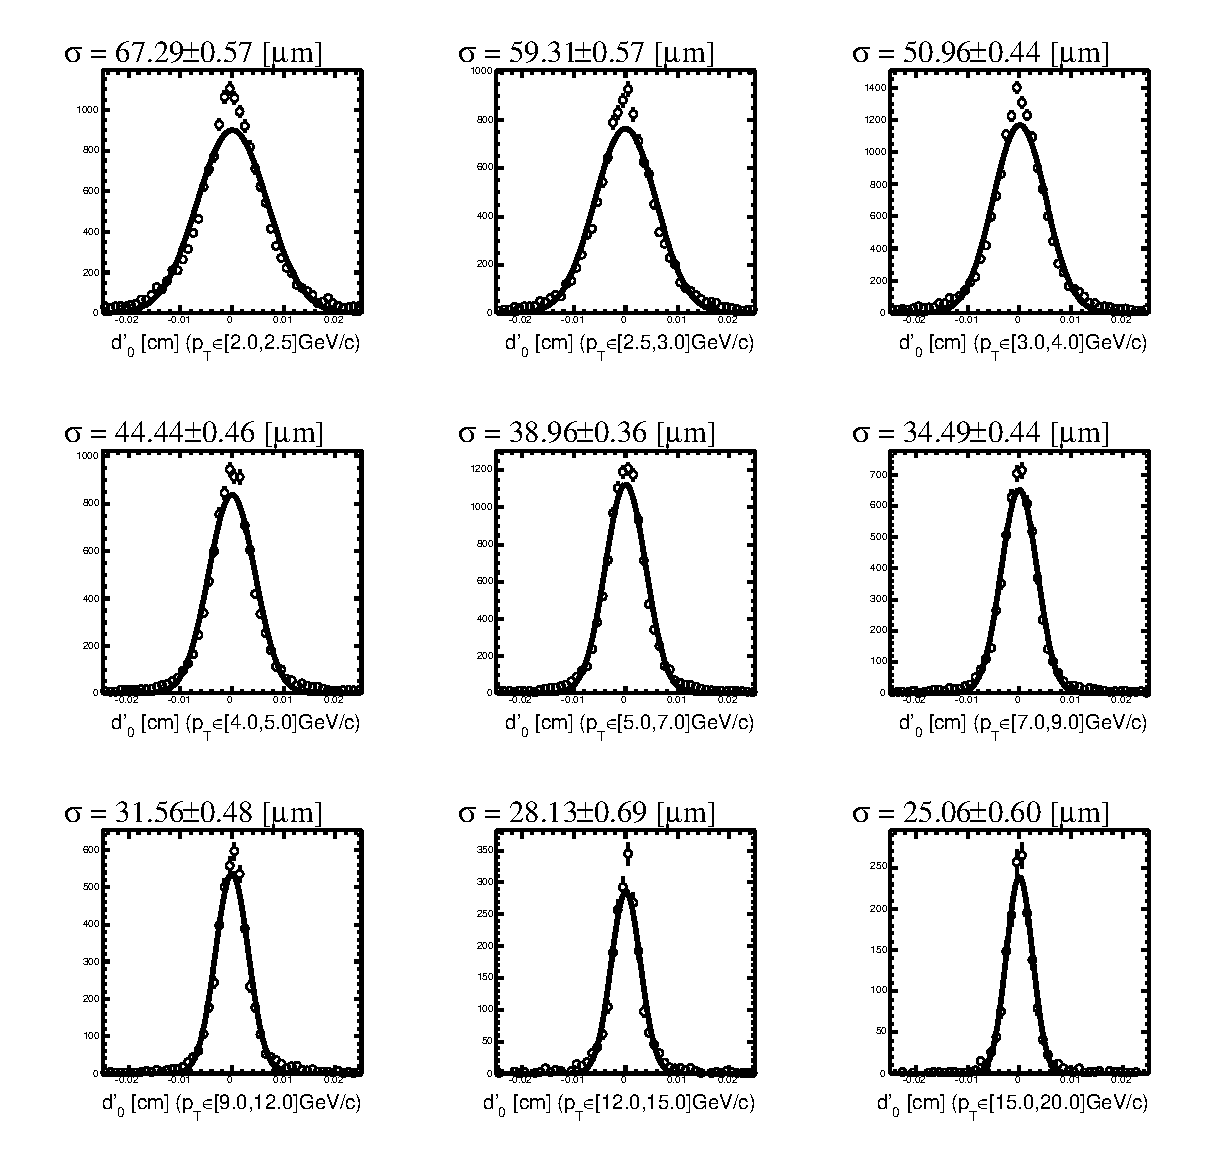
\includegraphics[width=0.85\textwidth]{figures/fxy_d0prime_array.eps}
      
    \caption{\it Distribution of reconstructed $d'_{0}$ (impact parameter in the beam reference frame, see ~\ref{sec:width} )
      in bins of $p_{T}$ obtained by the full MC simulation as described in \ref{sec:full_MC}.
      The track selection requirements are listed in Table \ref{TrackSelection}.
    }
    \label{fig:d0prime_array}
\end{figure}

\begin{figure}[htp]
  \centering
    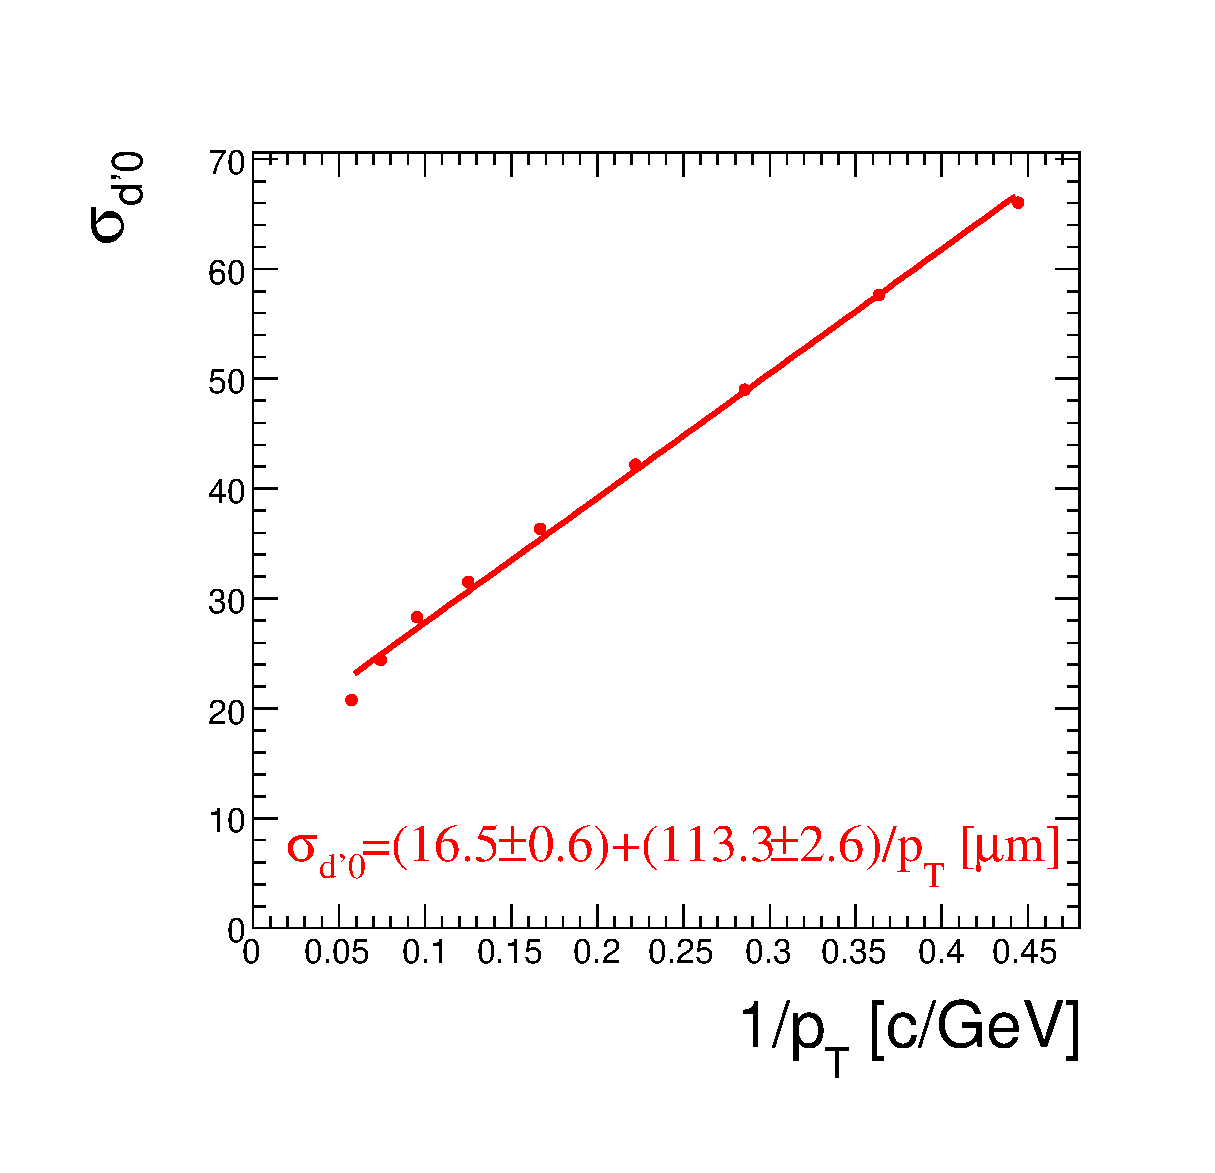
\includegraphics[width=0.6\textwidth]{figures/fxy_reso_d0prime_fit.eps}
      
    \caption{\it Impact parameter resolution averaged over all polar angles as function of $1/p_{T}$. The solid line is the 
      result of a linear fit. This result is obtained using the full MC simulation as described in Section \ref{sec:full_MC}.
    }
    \label{fig:reso_d0prime_fit}
\end{figure}

\begin{figure}[htp]
  \centering
    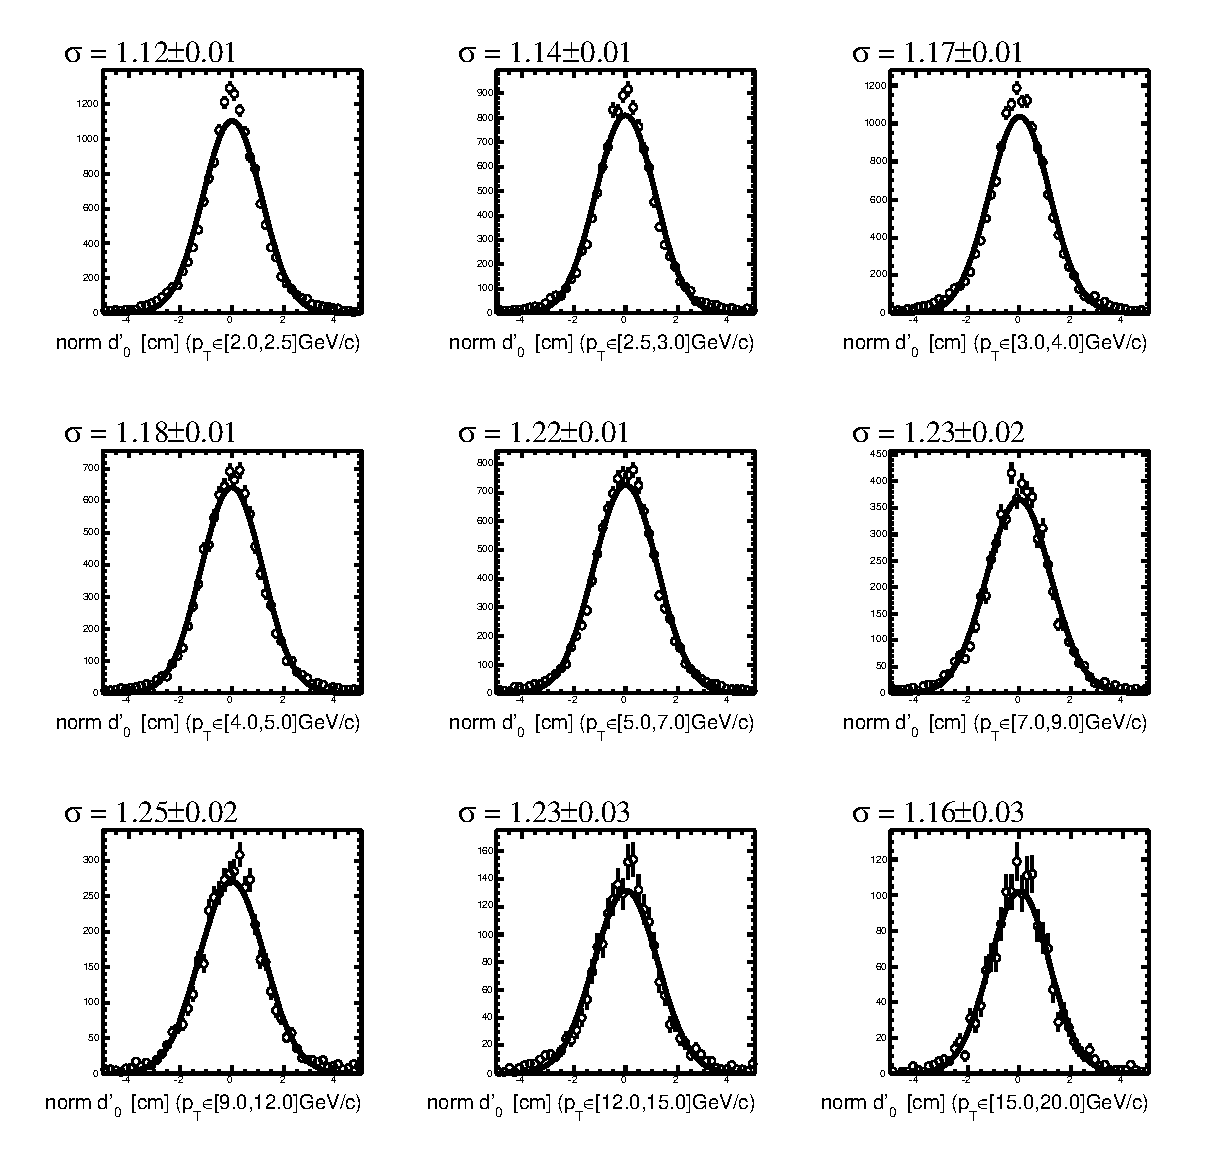
\includegraphics[width=0.9\textwidth]{figures/fxy_d0norm_array.eps}
      
    \caption{\it Distribution of reconstructed  $\frac{d'_{0}}{\sqrt{\sigma_{d_{0}}^2 +\sigma_{Beam}^2}}$ (normalized impact parameter in the beam reference frame, see ~\ref{sec:width} )
      in bins of $p_{T}$ obtained by the full MC simulation as described in \ref{sec:full_MC}. The track selection requirements are listed 
      in Table \ref{TrackSelection}.
    }
    \label{fig:normd0prime}
\end{figure}

\begin{figure}[htp]
  \centering
    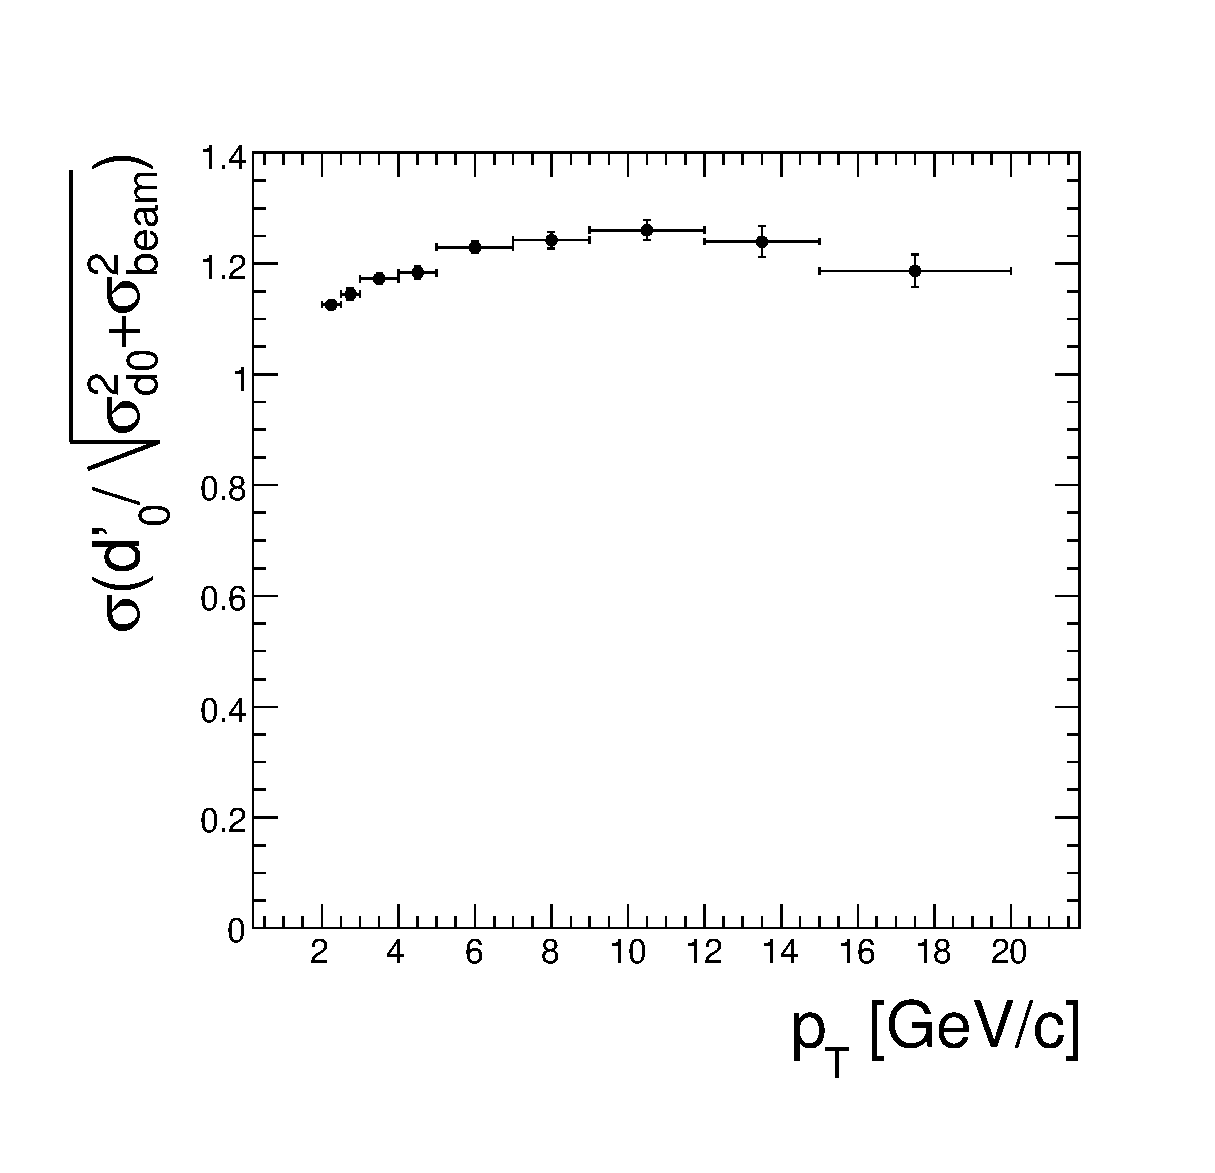
\includegraphics[width=0.6\textwidth]{figures/fxy_norm_sig.eps}
      
    \caption{\it  Gaussian width for the impact parameter pull distributions  as function of $p_{T}$.
 This result is obtained  using the full MC simulation as described in Section \ref{sec:full_MC}. 
    }
    \label{fig:norm_d0prime_fit}
\end{figure}


\clearpage
%\section{\label{sec:cdf}Applying the Log-likelihood {fitter} to extract the beam parameters to CDF data}

%At the Tevatron, the width of the beam varies significantly  and the longitudinal width of the beam provides us with a long lever arm
%, together with the excellent precision of the silicon vertex detector should allow us to extract the beam parameters $\beta^*$ and $\epsilon$.
%On the other hand, at the moment our fit does not take the detector acceptance into account, which will skew the $d_0 - \varphi_0$ correlation. 
%The CDF silicon detector consists of three barrels each with 29 cm long ladders leading to acceptance gaps in $z$ between the barrels. 
%In addition, there are some areas with ladders that do not function anymore. Figure \ref{fig:cdf} 
%gives an idea how the acceptance is skewed. The left plot in Figure \ref{fig:cdf} shows how the calculated impact parameter resolution 
%of selected tracks varies as a function of $z$. It clearly shows that the resolution gets worse as hits are lost on the boundary between 
%the barrels and the particles pass more material due to the part cards and hybrids located in this region. . The right plot in Figure  \ref{fig:cdf}
%shows how the selected tracks are distributed in $z$ representing a Gaussian sculptured by the geometric acceptance at the end cap and gap regions. 
%It is obvious that this distribution is not well represented by a Gaussian.

%Nonetheless we were very eager to try out the fit on real data but it is clear that a good modeling of the acceptance is necessary 
%to achieve good results. To allow for uncertainty in the scale factor of the calculated uncertainty of the impact parameter and to see how 
%sensitive the fit is to the error scale, we introduced scale factors for the error scale. Results with the different scale factors and different 
%data acquisition runs are summarized in Table \ref{table:cdfres} and the results are shown in Figure  \ref{fig:fitcdf} and compared to the expectation. 
 
 

%\begin{table} [th]
%\caption{\it \label{table:cdfsel} Track selection criteria.}
%\begin{center}
%\begin{tabular}{|l|c|} \hline
%\# of  Hits in Silicon Tracker                 & $>$ 3\\
%Transverse momentum                            & $>$ 2.0 GeV/c\\
%\# of axial Hits in central Tracking chamber   & $>$ 15\\
%\# of stereo Hits in central Tracking chamber  & $>$ 10\\
%estimated IP resolution                        & $<$ 60 $\mu$m\\
%absolute value of IP                           & $<150 \mu$m\\
%\hline
%\end{tabular}
%\end{center}
%\end{table}
 


%\begin{figure}[hbtp]
%  \begin{center}
%   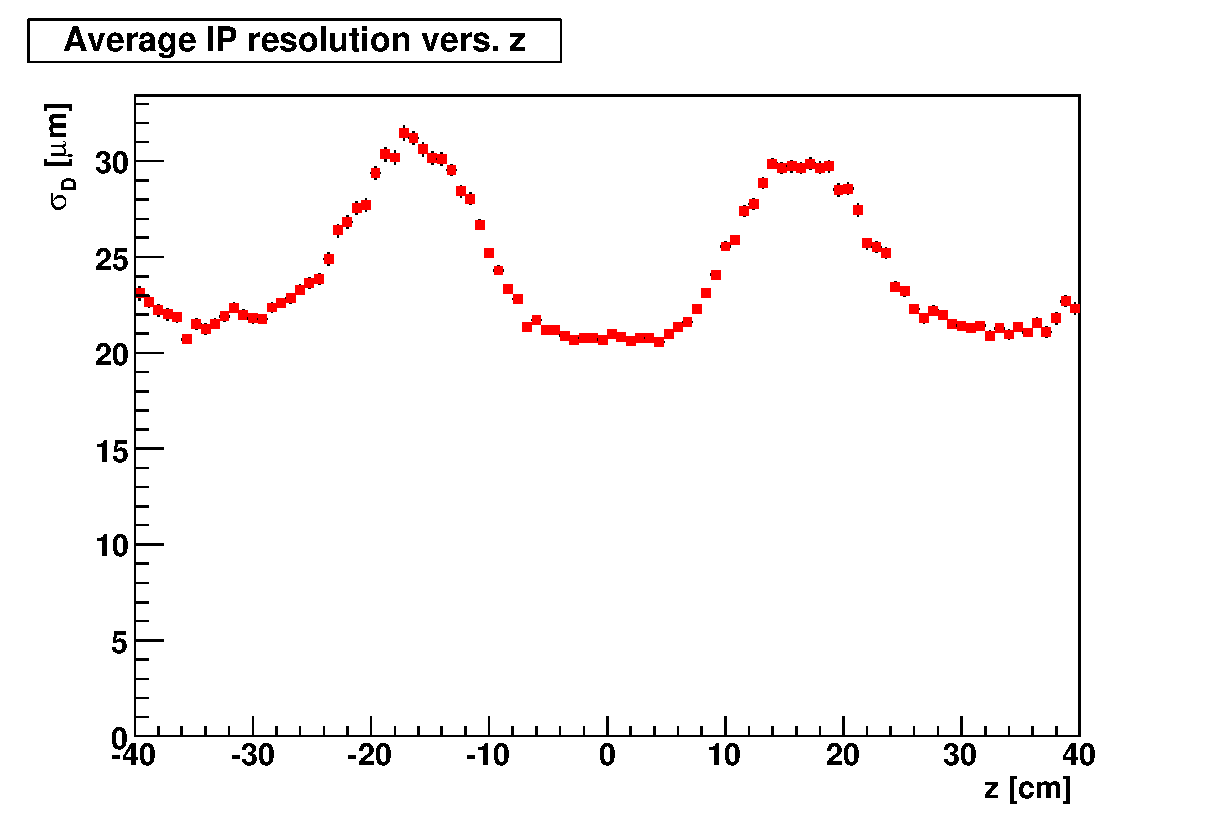
\includegraphics[width=0.45\textwidth]{figures/cdfsigd.eps}
%    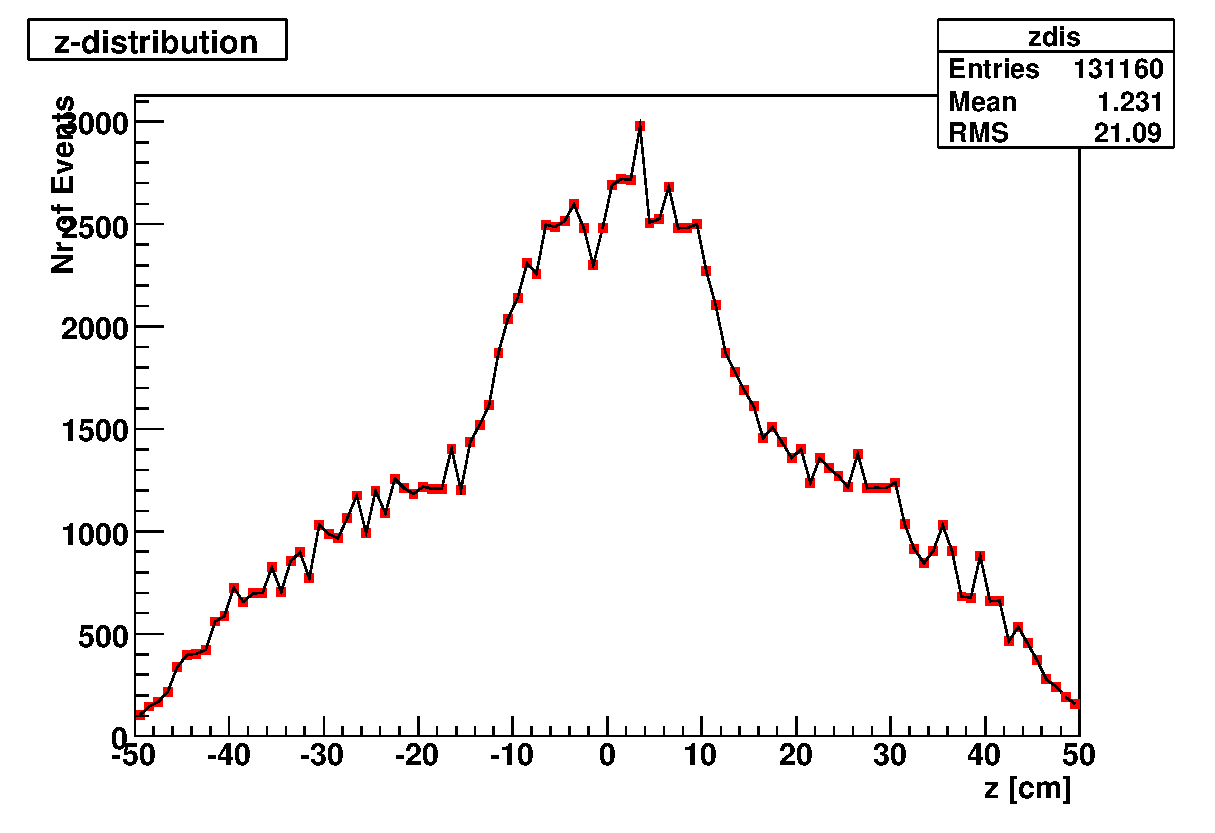
\includegraphics[width=0.45\textwidth]{figures/zdis.eps}
%    \caption{\it Average estimated impact parameter resolution (left)  and fitted z position (right) for the tracks
% for the tracks passing the selection criteria in listed in Table \ref{table:cdfsel}
%}
%    \label{fig:cdf}
%  \end{center}
%\end{figure}




%\begin{table} [th]
%\begin{center}
%\caption{\it \label{table:cdfres} Beam parameter fit results for different CDF data acquisition runs and  different IP error scale factors.}
%\begin{tabular}{|l|c|c|c|c|c|c|} \hline
%Run / Nr. of Tracks  & \multicolumn{2}{|c|}{Scale factor: 1}& \multicolumn{2}{|c|}{Scale factor: $\sqrt{2}$}& \multicolumn{2}{|c|}{Scale factor: $\sqrt{3}$} \\ \hline
%                     & $\epsilon$ & $\beta^*$               &  $\epsilon$ & $\beta^*$                        &  $\epsilon$ & $\beta^*$               \\ 
%                     & $[ 10^{-7}]$ & [cm]  & $[ 10^{-7}]$ & [cm]  & $[ 10^{-7}]$ & [cm]\\
%\hline
%197808/131160        & $2.21\pm 0.04$ & $56.9 \pm 1.3$  &   $1.69\pm 0.03$ & $48.2 \pm 1.2$  &  $1.24\pm 0.02$ & $40.6 \pm 1.2$  \\
%197657/28588         & $2.22\pm 0.09$ & $57.9 \pm 2.3$  &   $1.73\pm 0.07$ & $48.8 \pm 2.6$  &  $1.30\pm 0.05$ & $41.0 \pm 2.4$  \\
%197763/89806         & $2.39\pm 0.05$ & $55.3 \pm 1.4$  &   $1.86\pm 0.04$ & $47.7 \pm 1.3$  &  $1.41\pm 0.03$ & $41.1 \pm 1.3$  \\
%\hline
%\end{tabular}
%\end{center}
%\end{table}



%\begin{figure}[hbtp]
%  \begin{center}
%    \resizebox{10cm}{!}{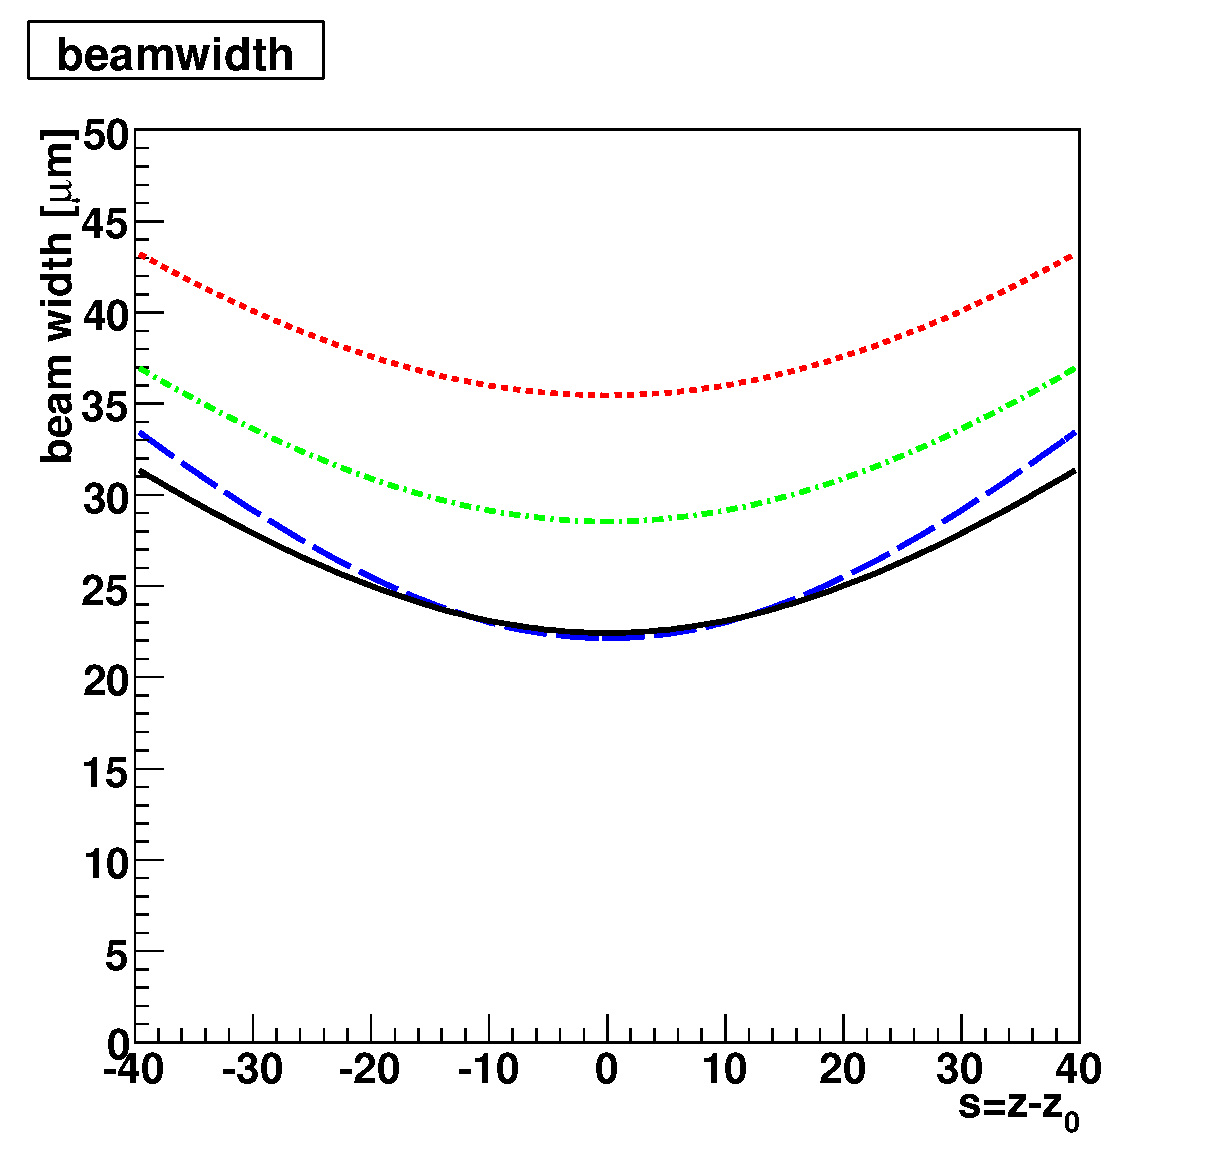
\includegraphics{figures/fitcdf.eps}}
%    \caption{\it Fitted $\beta$-function for different scale factors. The solid (black) line represents the expected value. 
%      The dashed lines from top to bottom represent a scale factor of the resolution of 1 (red) , $\sqrt{2}$ (green) and $\sqrt{3}$ (blue).}
%    \label{fig:fitcdf}
%  \end{center}
%\end{figure}


\clearpage
\section{Conclusions}
The work presented in this note shows that the beam position and 
width can be determined with algorithms based solely on track information.
A statistical precision of 2 $\mu$m  can be achieved for the average transverse
beam position with only one thousand tracks that pass the selection criteria. 
Assuming that the beam width does not vary with
$z$ throughout the interaction region, it can also be 
measured with 20 \% precision with the same track sample.
The determination of the beam width requires good understanding of the impact parameter uncertainties as returned 
by the track fit. 




The $d_0 - \varphi_0$ algorithm is fast and robust against large beam displacements. 
It allows the determination of the beam offsets and angles reasonably well 
without the pixel system, 
while the beam width, $\beta^{*}$ and emittance require the tracking precision provided by the pixel detector.
The  $d_0 - \varphi_0$ fitter is ideally suited to monitor the beam during data 
taking as has been  done by CDF 
for many years. 

Once the beam parameters are determined with high precision this information can be used to study the track impact parameter
resolution. 

For the purpose of these studies the CMS detector simulation was expanded to include a more realistic simulation of the event vertex distribution. 
This included beam offsets in $x$, $y$ and $z$ from the nominal center of the detector; angles with respect to the 
detector $z$-axis and the interaction vertex to be distributed according to the $\beta$-function. The
fit algorithms have been implemented in the CMS reconstruction software and an interface to write and read the
beam spot data to and from the database has been developed.






\section{\label{sect:acknowledgments}Acknowledgments}

We would like to thank Kevin Burkett, Hans Jensen and Lenny Spiegel (FNAL) 
for proof-reading this note. Thomas Speer, Jeff Spalding and Fabrizio served as referees and editor of this note. Hartmut Stadie (DESY) provided us with some of 
the C++ code. Francesco Ruggiero (CERN) provided us with references regarding the LHC beam parameters, we were saddened to hear the news that he 
passed away on the $17^{th}$ of January.

%\section{Preliminary result }

%In this section, we describe the potential of using CMS  tracks for the 
%purpose of beam profile calculation and also other studies such as tracking resolution 
%measurement and tracker alignment.     A standalone version~\cite{pythia6} of \pythia embedded in ROOT  is used 
%for the event generation.  For each event, a 3-dimensional primary vertex position is 
%simulated using three Gaussian resolution functions with the width of the Gaussian as 
%the beam profile in X,Y and Z directions. The beam profile in Z is assumed as a single 
%Gaussian with the width $\sigma_z$ in different beam scenarios as in Table~\ref{table:beams}. 
%The beam profiles in X and Y directions are assumed to follow the Gaussian functions as well but 
%with the width as function of projected $Z$ values described by the beta function,
%$\sigma^{b}(z-z_0) = \sqrt{\epsilon \beta^* \times (1+(z-z_0)/\beta^*)^2)}$. The values of 
%$\epsilon $ and  $\beta^*$ were taken from  Table~\ref{table:beams}. We use $z_0=0$ for the
%simplicity reason.     
%First, the event-by-event   primary vertex position 
%were shifted using a pre-defined averaged beam positions relative 
%to the CMS detector center  in x and y. The values of the averaged beam x-y positions are to 
%be extracted from the $d-\varphi$ fitting program.  We assumed a range of the beam position 0 to 2mm 
%in the simulation.   For simplicity, we fixed the beam position on Z direction as $z_0 = 0$. 
%Next, the primary vertex position is smeared with the beam profiles described either by a 
%simple Gaussian function with a fixed width in Z-direction or a Gaussian function with a width 
%of a beta function. 
%Then, tracks within pseudo-rapidity of 2.5 were collected  
%and  their production  vertex position is shifted using the event-by-event  primary vertex.
%The helix parameter of these tracks were calculated in a homogeneous magnetic field of 4~Tesla 
%assuming a circular trajectory in x-y plane.  In the calculation of helix parameters, the tracks 
%were assumed coming from the CMS detector center. 
%Finally, the calculated helix parameters such as $D$, $\varphi_0$ and $z_0$ were smeared using 
%Gaussian resolution functions with width taken from Table~\ref{IPresolution}
\clearpage




{\Large \bf Appendix 1}

An additional check has been done varying the beam position over a wide range. This allows for displacement of several mm from the nominal detector 
coordinate system. Table \ref{table:BeamSpotLHC2008} summarizes the results
for a sample generated with the LHC nominal configuration. Table \ref{table:BeamSpotNopixelLHC2008} shows the results for the case without pixel detector.

\begin{table} [th]
\caption{\it \label{table:BeamSpotLHC2008} Beam Position fitting result with pixel in CMS tracker. Beam profile 
were generated using parameters $\beta^* =  55~cm$, $\epsilon=3.75 \times 10^{-8}$ and 
$\sigma_z=7.55~cm$ as expected for the nominal LHC stable runs. About 950K tracks with $p_T>2$~GeV/c were 
used in each fit.}
\begin{center}
\begin{tabular}{|c|c|c|c|c|c|c|c|} \hline
\multicolumn{4}{|c|}{Input values}& \multicolumn{4}{|c|}{Fitted  values}\\ \hline
$x_0$& $y_0$& $dx/dz$&$dy/dz$ &  $x_0$(Fit) & $y_0$ (Fit) & $dx/dz$ (Fit) & $dy/dz$ (Fit) \\
~[$\mu$m] & ~[$\mu$m] & ~[$\mu$m/cm] & ~[$\mu$m/cm] & ~[$\mu$m] & ~[$\mu$m] & ~[$\mu$m/cm] & ~[$\mu$m/cm] \\ \hline
0   & 0   & 0 &    0 &$ 0.110  \pm 0.047$&$-0.004  \pm 0.047$&$1.08 \pm 0.63   $&$  1.15 \pm  0.63$\\ \hline
100 & 300 & 0 &    0 &$ 100.011\pm 0.047$&$300.006 \pm 0.047$&$0.59 \pm 0.63   $&$ -0.22 \pm  0.63 $\\ \hline
300 & 600 & 0 &    0 &$ 299.982\pm 0.047$&$600.05  \pm 0.047$&$0.02 \pm 0.63   $&$  0.15 \pm  0.63 $\\ \hline
600 & 900 & 0 &    0 &$ 600.064\pm 0.047$&$899.928 \pm 0.047$&$0.43 \pm 0.63   $&$  0.23 \pm  0.63 $\\ \hline
900 & 1200& 0 &    0 &$ 900.071\pm 0.047$&$1199.96 \pm 0.047$&$-0.81 \pm 0.63  $&$ -0.65 \pm  0.63$\\ \hline
1200& 1500& 0 &    0 &$ 1200.03\pm 0.047$&$1500.04 \pm 0.047$&$0.15  \pm  0.63 $&$  0.31 \pm  0.63$\\ \hline
1500& 2000& 0 &    0 &$ 1500.00\pm 0.047$&$1999.97 \pm 0.047$&$-0.49 \pm  0.63 $&$ -0.03 \pm  0.63$\\ \hline
2000& 3000& 0 &    0 &$ 1999.91\pm 0.047$&$3000.02 \pm 0.047$&$0.13  \pm  0.63$&$  -0.35 \pm  0.63$\\ \hline
3000& 4000& 0 &    0 &$ 3000.03\pm 0.047$&$4000.04 \pm 0.047$&$0.15  \pm  0.62 $&$ -0.74 \pm  0.63$\\ \hline
4000& 5000& 0 &    0 &$ 3999.92\pm 0.047$&$4999.96 \pm 0.047$&$0.08  \pm  0.62 $&$ -0.40 \pm   0.62$\\ \hline
300 & 600 & 10&    30&$ 300.048\pm 0.047$&$599.938 \pm 0.047$&$10.41 \pm  0.63 $&$ 30.14 \pm   0.63$\\ \hline
300 & 600 & 30&    60&$ 299.991\pm 0.047$&$599.907 \pm 0.047$&$30.32 \pm  0.63 $&$ 60.13 \pm   0.63$\\ \hline
300 & 600 & 60&    90&$ 300.04 \pm 0.047$&$600.012 \pm 0.047$&$61.71 \pm  0.63 $&$ 91.65 \pm   0.63$\\ \hline
300 & 600 & 90&   120&$ 300.014\pm 0.047$&$599.949 \pm 0.047$&$90.20 \pm  0.63 $&$ 120.25 \pm  0.63$\\ \hline
300 & 600 &120&   150&$ 300.017\pm 0.047$&$599.975 \pm 0.047$&$120.63\pm  0.63 $&$ 150.78 \pm  0.63$\\ \hline
300 & 600 &150&   180&$ 299.998\pm 0.048$&$599.983 \pm 0.047$&$148.74 \pm 0.63 $&$ 179.35\pm   0.63$\\ \hline
300 & 600 &180&   210&$ 299.958\pm 0.048$&$599.985 \pm 0.047$&$180.29\pm  0.63 $&$ 209.73 \pm  0.63$\\ \hline
\end{tabular}


\end{center}
\end{table}


%\begin{figure}[hbtp]
%   \caption{\it Beam Position fitting result with pixel in CMS tracker in LHC 2008 stable runs. Results from
%    Table \ref{table:BeamSpotLHC2008}.}
%  \begin{center}
%    \resizebox{6cm}{!}{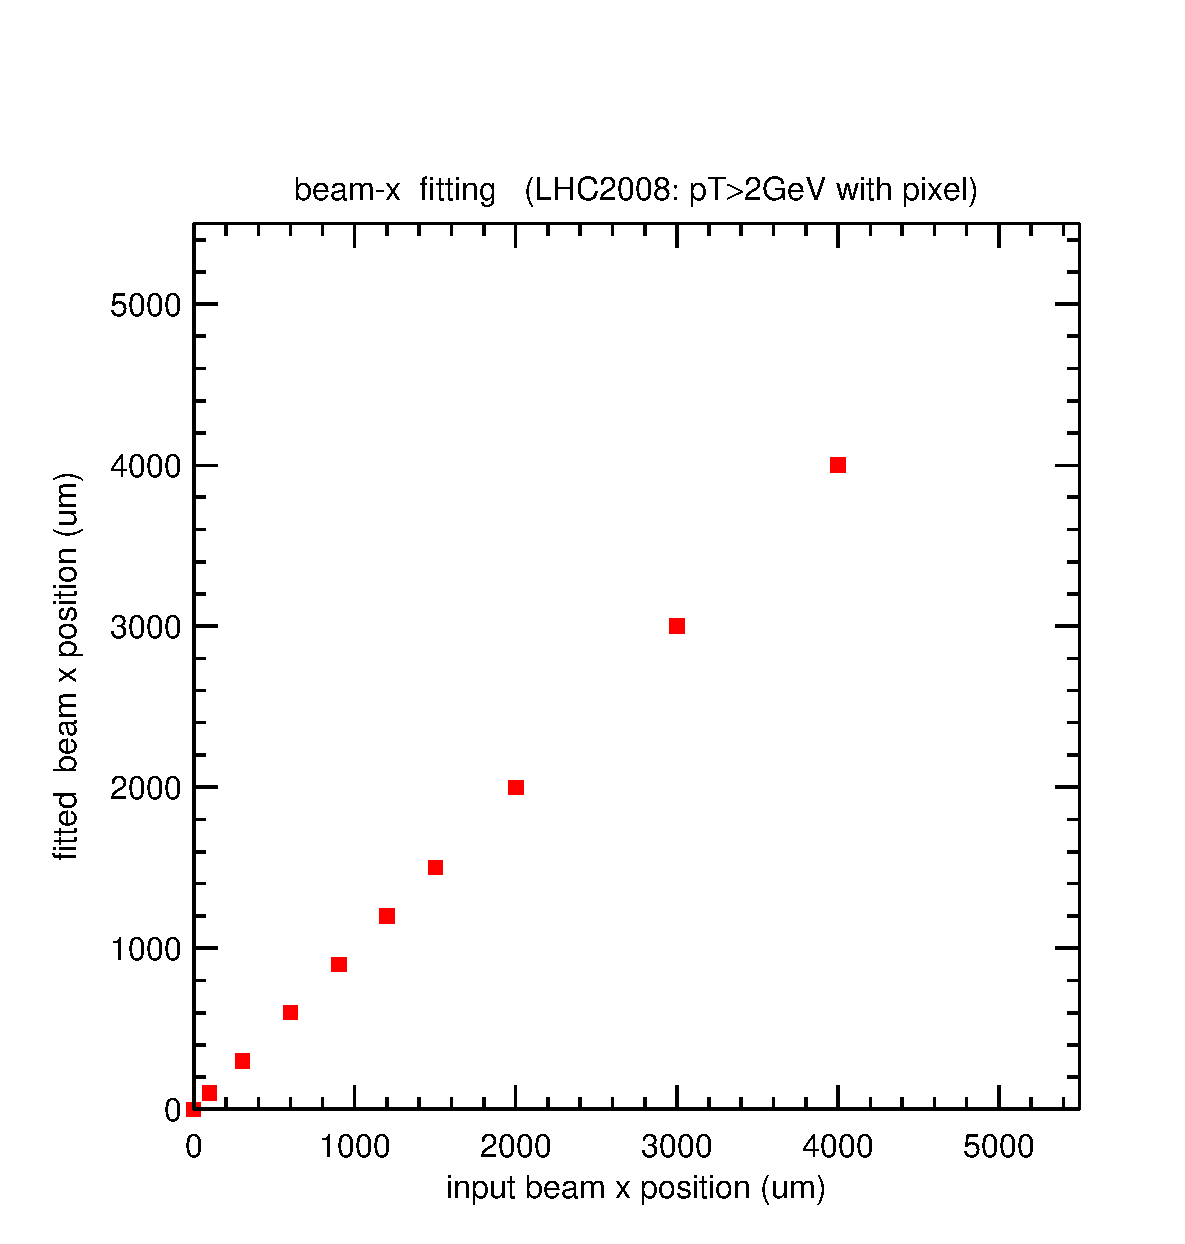
\includegraphics{figures/beam_x_fit.eps}}
%    \resizebox{6cm}{!}{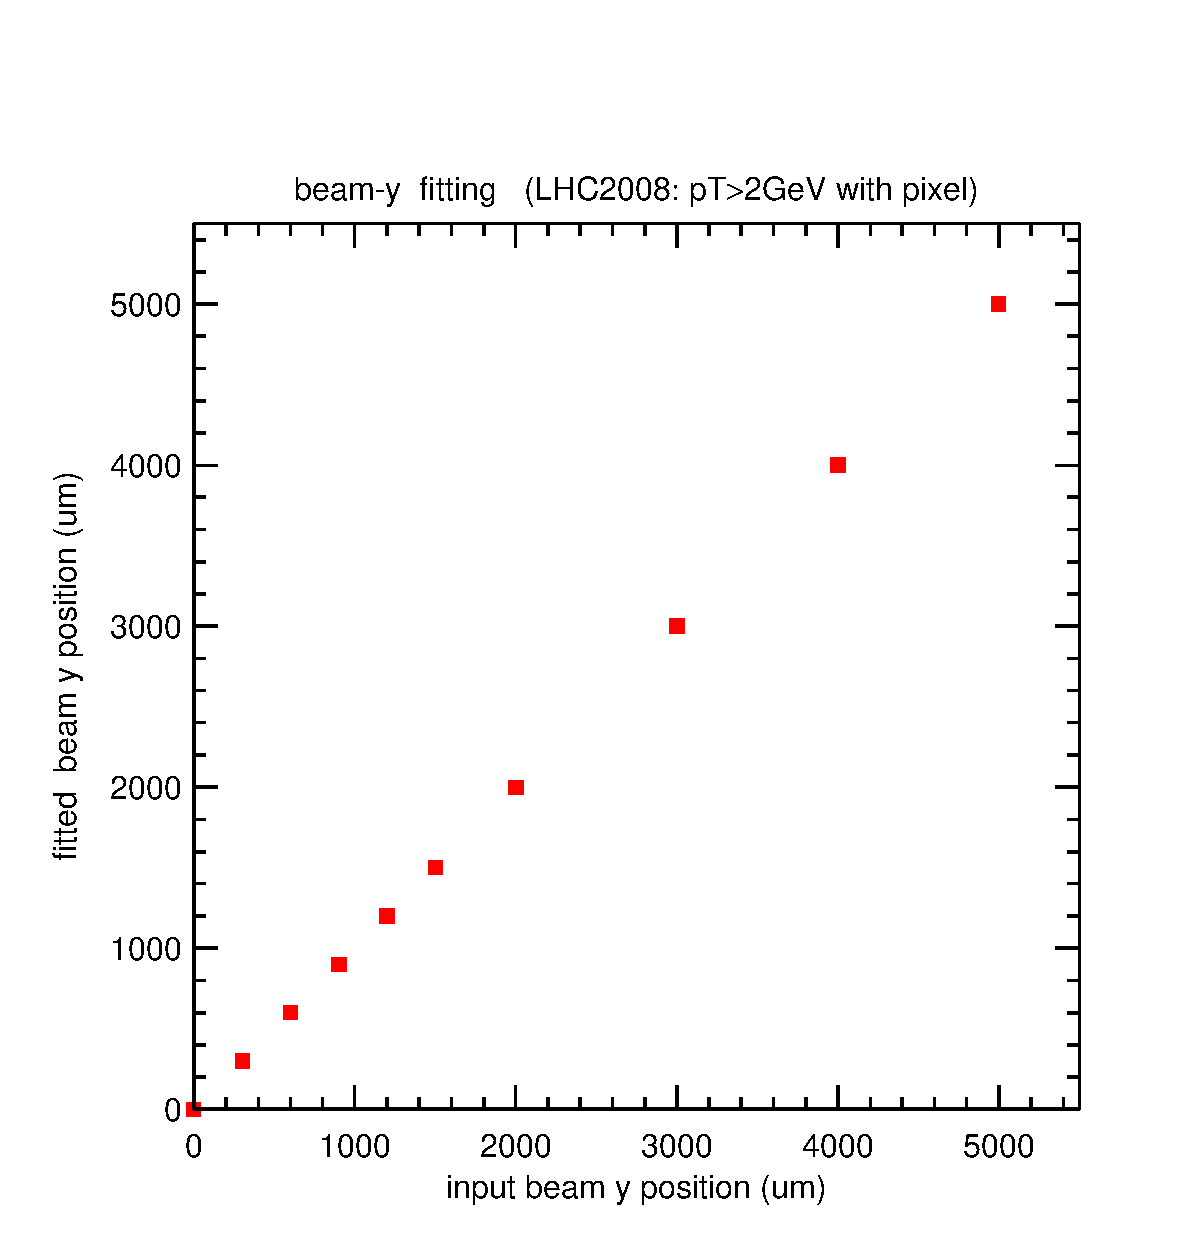
\includegraphics{figures/beam_y_fit.eps}}
%    \resizebox{6cm}{!}{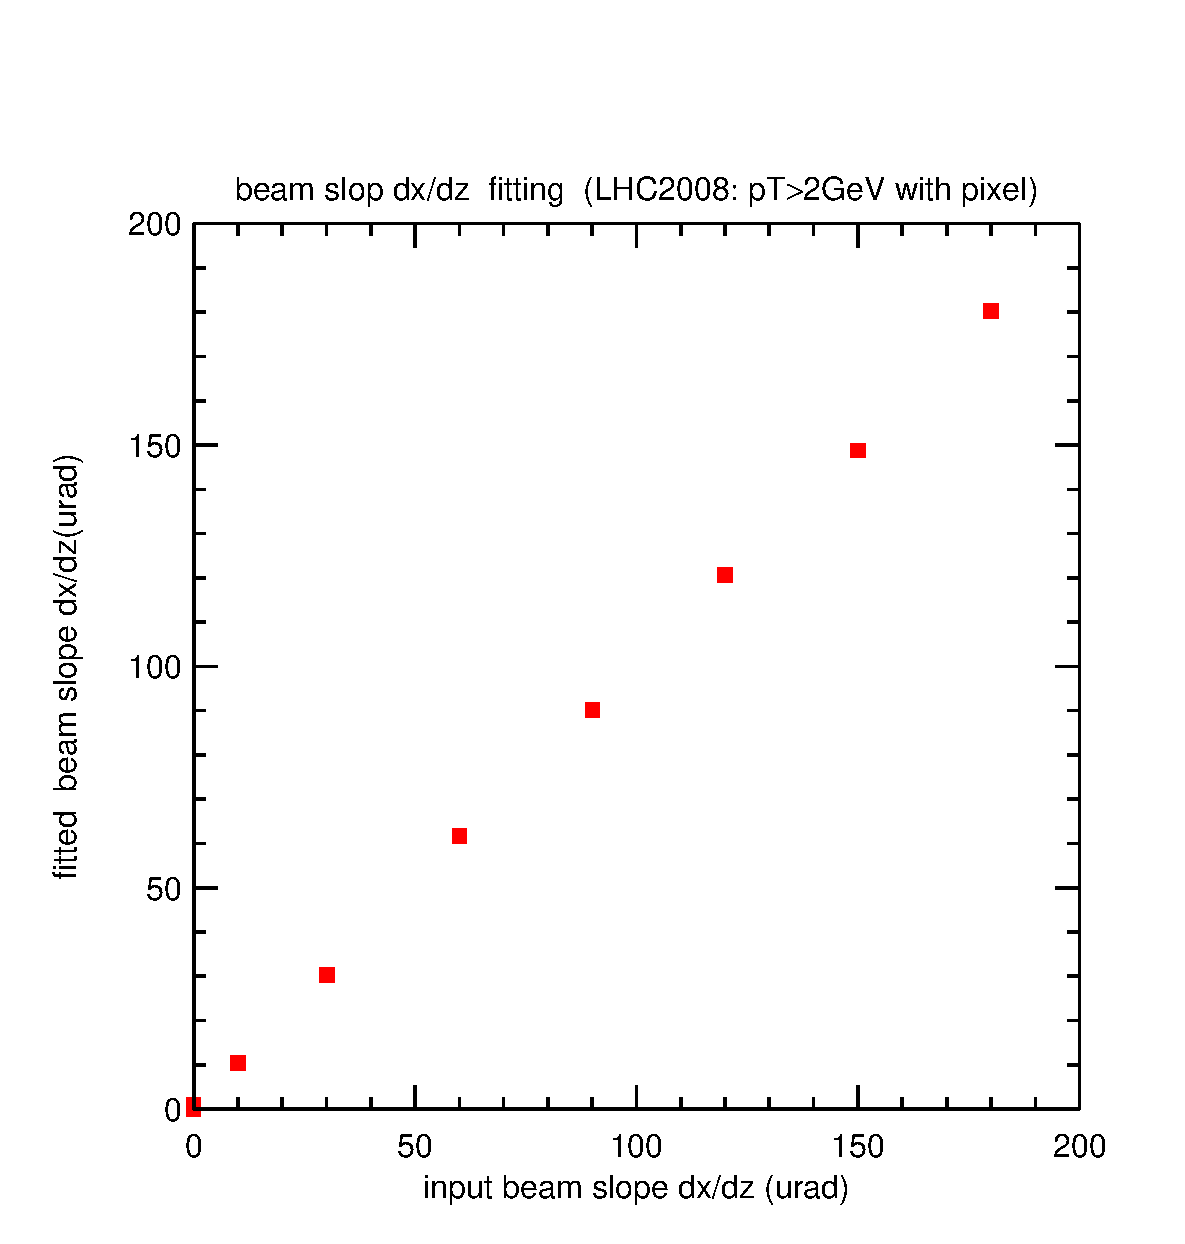
\includegraphics{figures/beam_xslope_fit.eps}}
%    \resizebox{6cm}{!}{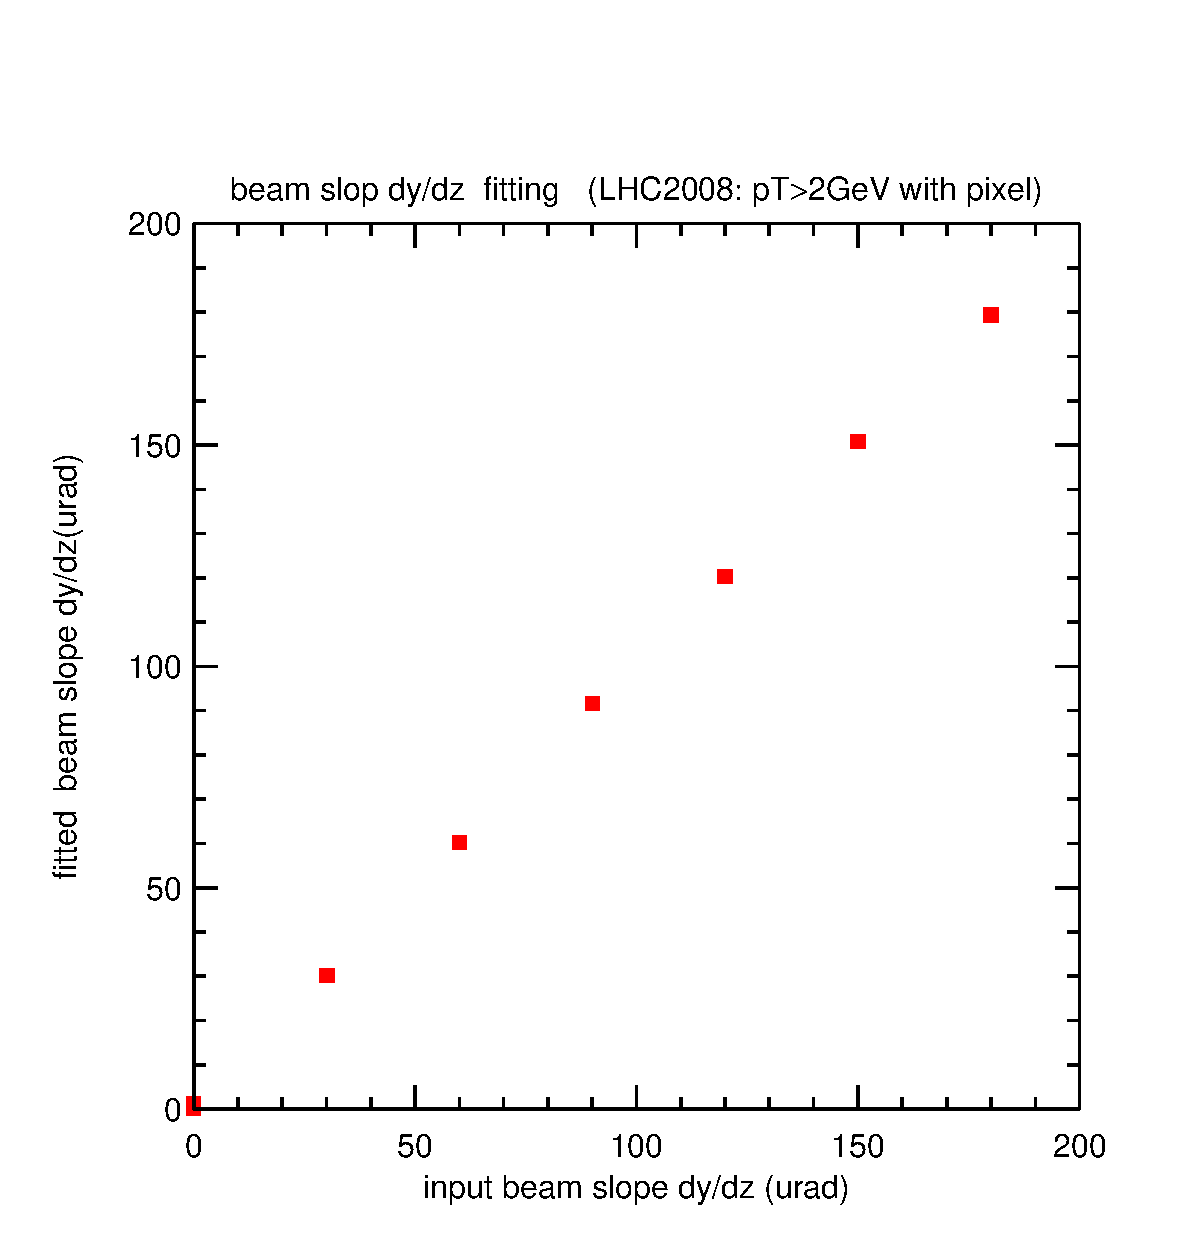
\includegraphics{figures/beam_yslope_fit.eps}}
%    \label{fig:BeamSpotLHC2008}
%  \end{center}
%\end{figure}




\begin{table} [th]

\caption{\it \label{table:BeamSpotNopixelLHC2008} Beam Position fitting result using tracks 
from CMS detector configuration without pixel.  Beam profile were generated using 
parameters $\beta^* =  55~cm$, $\epsilon=3.75 \times 10^{-8}$ and $\sigma_z=7.55~cm$ as 
expected for the nominal LHC stable runs. About 350K tracks with $p_T>5$~GeV/c were used 
in each fit.}
\begin{tabular}{|c|c|c|c|c|c|c|c|} \hline
\multicolumn{4}{|c|}{Input values}& \multicolumn{4}{|c|}{Fitted  values}\\ \hline
$x_0$& $y_0$& $dx/dz$&$dy/dz$ &  $x_0$(Fit) & $y_0$ (Fit) & $dx/dz$ (Fit) & $dy/dz$ (Fit) \\ 
%[\$mu$ m] &[\$mu$ m] &[\$mu$ m/cm] &[\$mu$ m/cm] &[\$mu$ m] &[\$mu$ m] &[\$mu$ m/cm] &[\$mu$ m/cm] \\ \hline
~[$\mu$m] & ~[$\mu$m] & ~[$\mu$m/cm] & ~[$\mu$m/cm] & ~[$\mu$m] & ~[$\mu$m] & ~[$\mu$m/cm] & ~[$\mu$m/cm] \\ \hline
0  &  0 & 0&     0&$  0.03  \pm    0.30$&$ -0.63\pm 0.29 $&$ 2.2 \pm  3.9  $&$ 2.9 \pm  3.9 $ \\ \hline
100& 300& 0&     0&$  100.335\pm   0.30$&$ 300.05 \pm  0.29 $&$ 8.1 \pm  3.9  $&$ -5.6\pm   3.9  $ \\ \hline
300& 600& 0&     0&$  300.33 \pm   0.30$&$ 600.047 \pm  0.29 $&$ 3.1 \pm  3.9  $&$-3.4 \pm  3.9  $ \\ \hline
600& 900& 0&     0&$  600.29\pm   0.30$&$ 899.969 \pm  0.30$&$ -1.7 \pm  3.9 $&$  1.3 \pm  3.9  $ \\ \hline
900& 1200&0&     0&$  899.78 \pm   0.30$&$ 1199.93 \pm  0.29 $&$-2.2  \pm 3.9  $&$ 1.9 \pm  3.9  $ \\ \hline
1200&1500&0&     0&$  1200.04\pm   0.30$&$ 1499.89 \pm  0.30 $&$  3.8 \pm  3.9 $&$  1.3 \pm  3.9  $ \\ \hline
1500&2000&0&     0&$  1500.31 \pm  0.30$&$ 1999.65 \pm  0.29 $&$-3.0  \pm 3.9  $&$-4.0 \pm  3.9  $ \\ \hline
2000&3000&0&     0&$  1999.93 \pm  0.30$&$ 3000.4  \pm  0.29 $&$ 4.2 \pm  3.9  $&$-0.3\pm  3.9 $ \\ \hline 
3000&4000&0&     0&$  3000.24 \pm  0.30$&$ 3999.98 \pm  0.29 $&$-3.0 \pm  3.9  $&$ 6.2 \pm  3.9 $ \\ \hline 
4000&5000&0&     0&$  3999.76 \pm  0.30$&$ 4999.94 \pm  0.29 $&$ 4.6 \pm  3.9  $&$-2.8  \pm 3.9  $ \\ \hline
300& 600& 10&    30&$ 300.60  \pm  0.30$&$ 599.941  \pm 0.29 $&$ 17.2 \pm  3.9  $&$  29.9 \pm 3.9  $ \\ \hline
300& 600& 30&    60&$ 300.04 \pm   0.30$&$ 599.881  \pm 0.29 $&$ 33.0 \pm  3.9  $&$ 59.9\pm 3.9  $ \\ \hline
300& 600& 60&    90&$ 300.03 \pm   0.30$&$  599.641 \pm 0.29 $&$  65.9\pm  3.9   $&$ 87.1 \pm 3.9  $ \\ \hline
300& 600& 90&   120&$ 299.97 \pm   0.30$&$ 599.827  \pm 0.29 $&$ 89.9 \pm  3.9   $&$120.2  \pm 3.9  $ \\ \hline
300& 600&120&   150&$ 300.44 \pm   0.30$&$ 599.847  \pm 0.29 $&$ 127.4 \pm  3.9  $&$ 153.1 \pm  3.9  $ \\ \hline
300& 600&150&   180&$ 299.83 \pm   0.30$&$ 600.491\pm 0.29 $&$ 146.2 \pm  3.9  $&$ 177.6  \pm  3.9  $ \\ \hline
300& 600&180&   210&$ 299.97 \pm   0.30$&$ 599.623  \pm 0.29 $&$  179.1\pm 3.9   $&$208.9  \pm 3.9  $ \\ \hline
\end{tabular}
\begin{center}

\end{center}
\end{table}


%\begin{figure}[hbtp]
%  \begin{center}
%    \resizebox{6cm}{!}{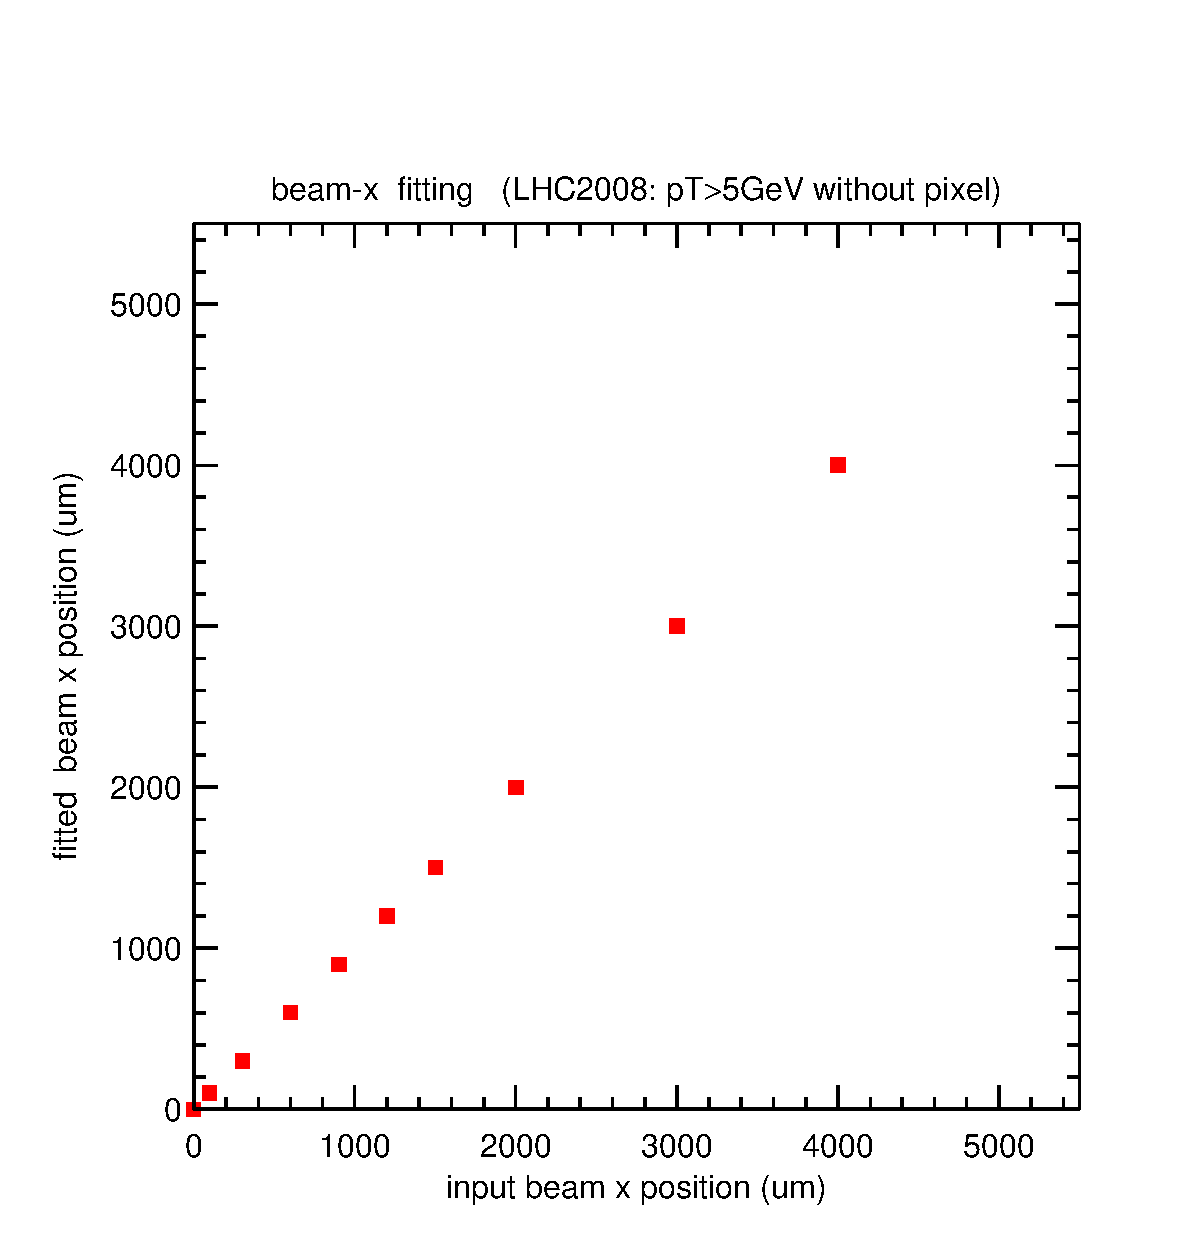
\includegraphics{figures/beam_x_fit_nopixel.eps}}
%    \resizebox{6cm}{!}{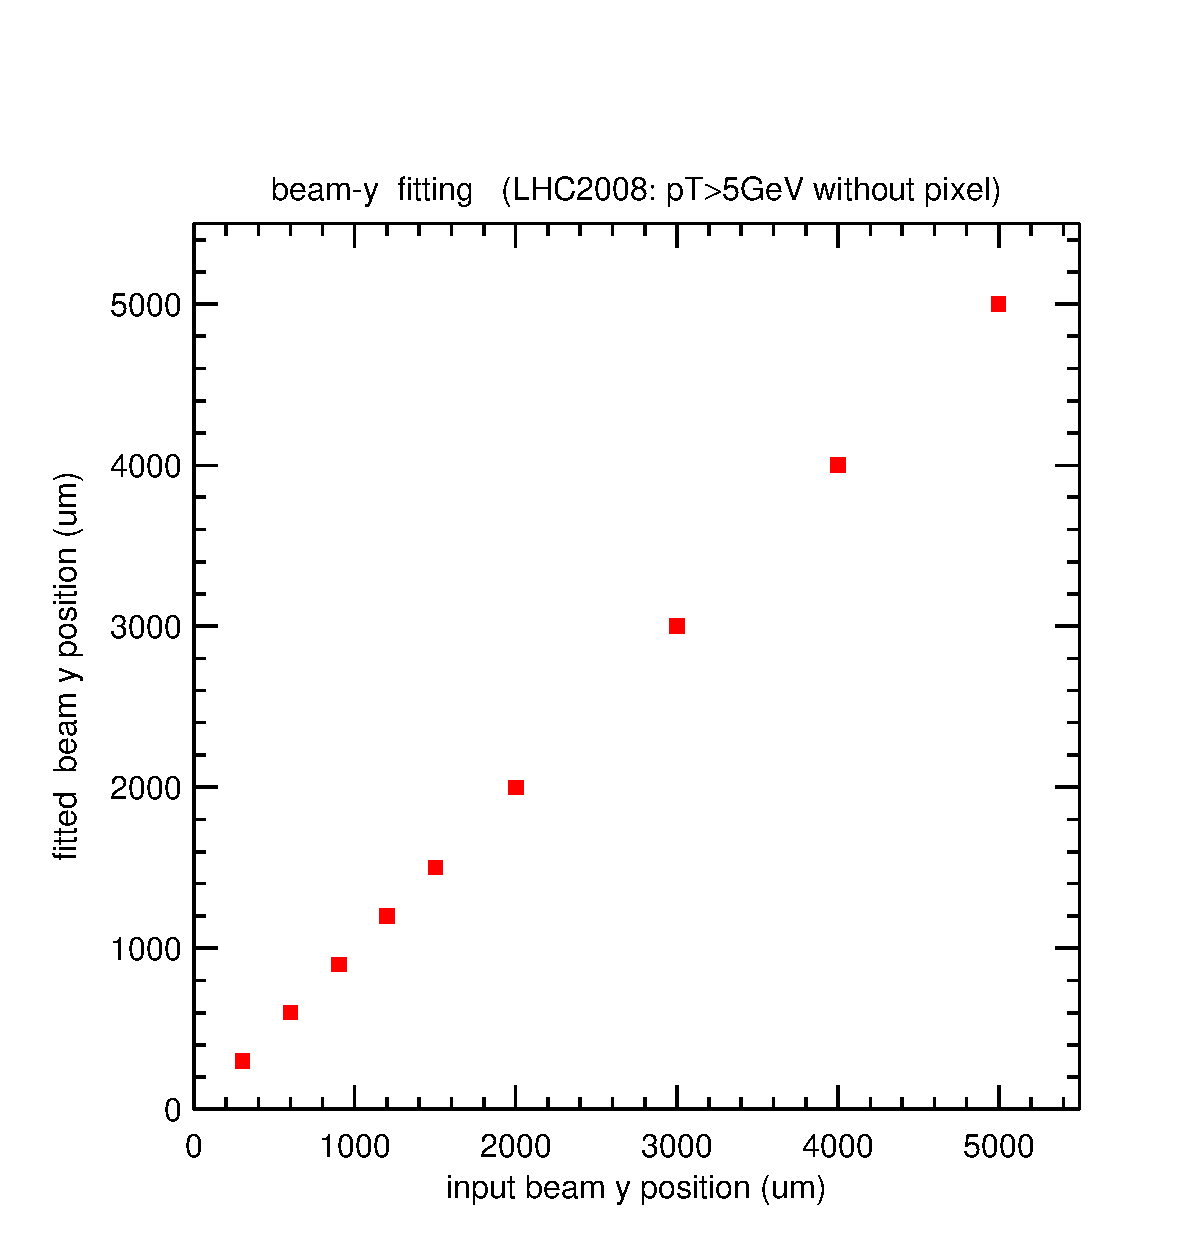
\includegraphics{figures/beam_y_fit_nopixel.eps}}
%    \resizebox{6cm}{!}{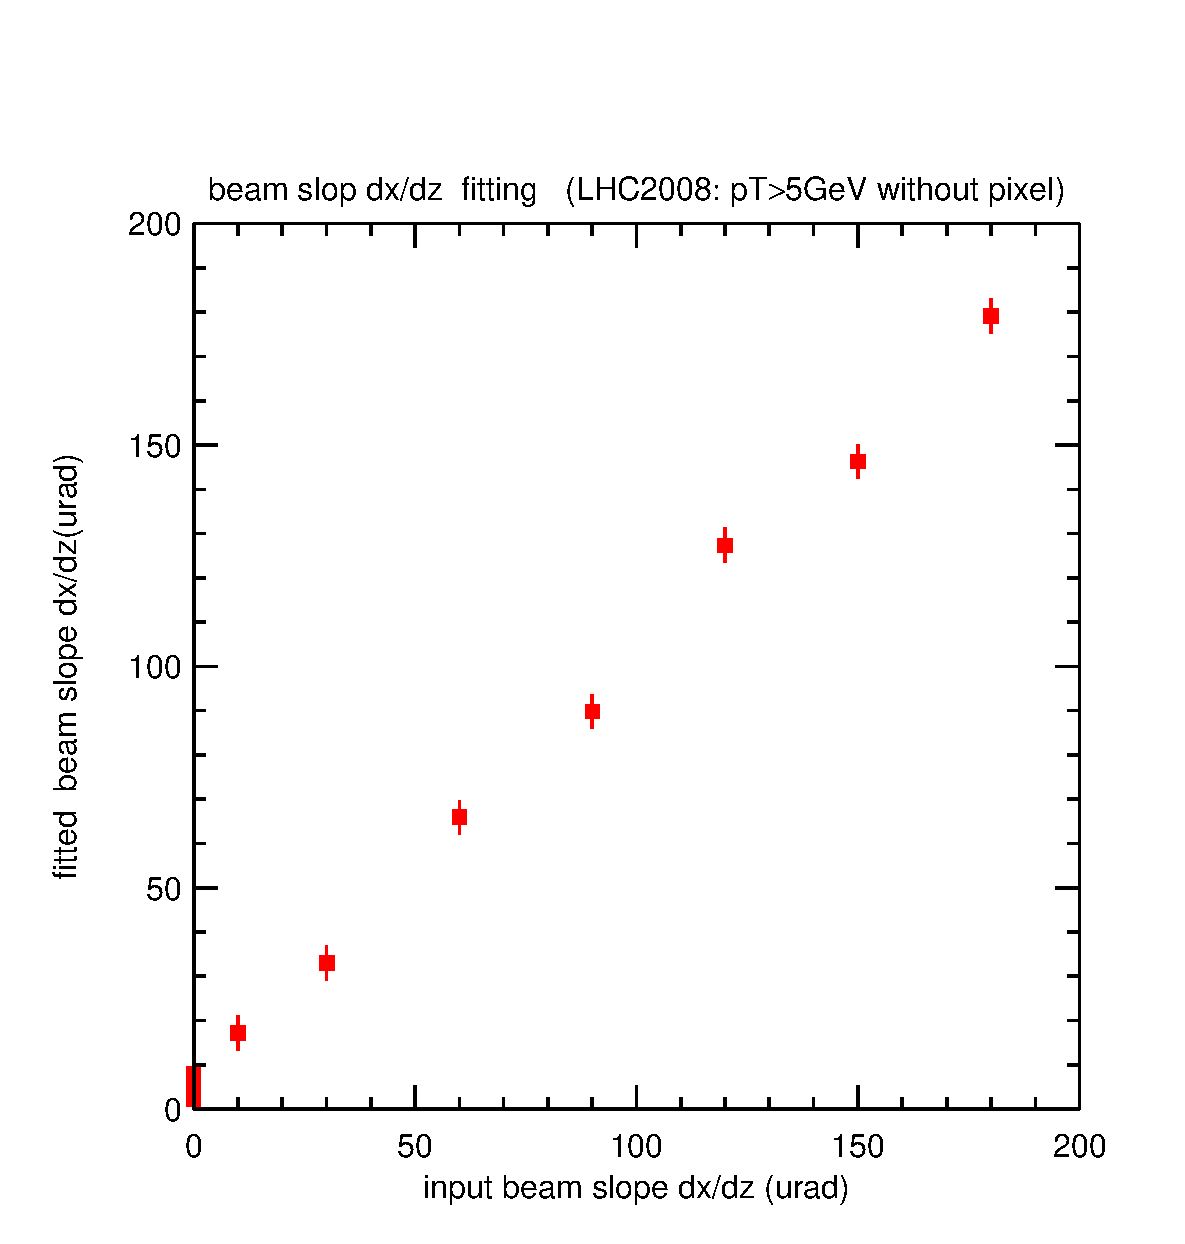
\includegraphics{figures/beam_xslope_fit_nopixel.eps}}
%    \resizebox{6cm}{!}{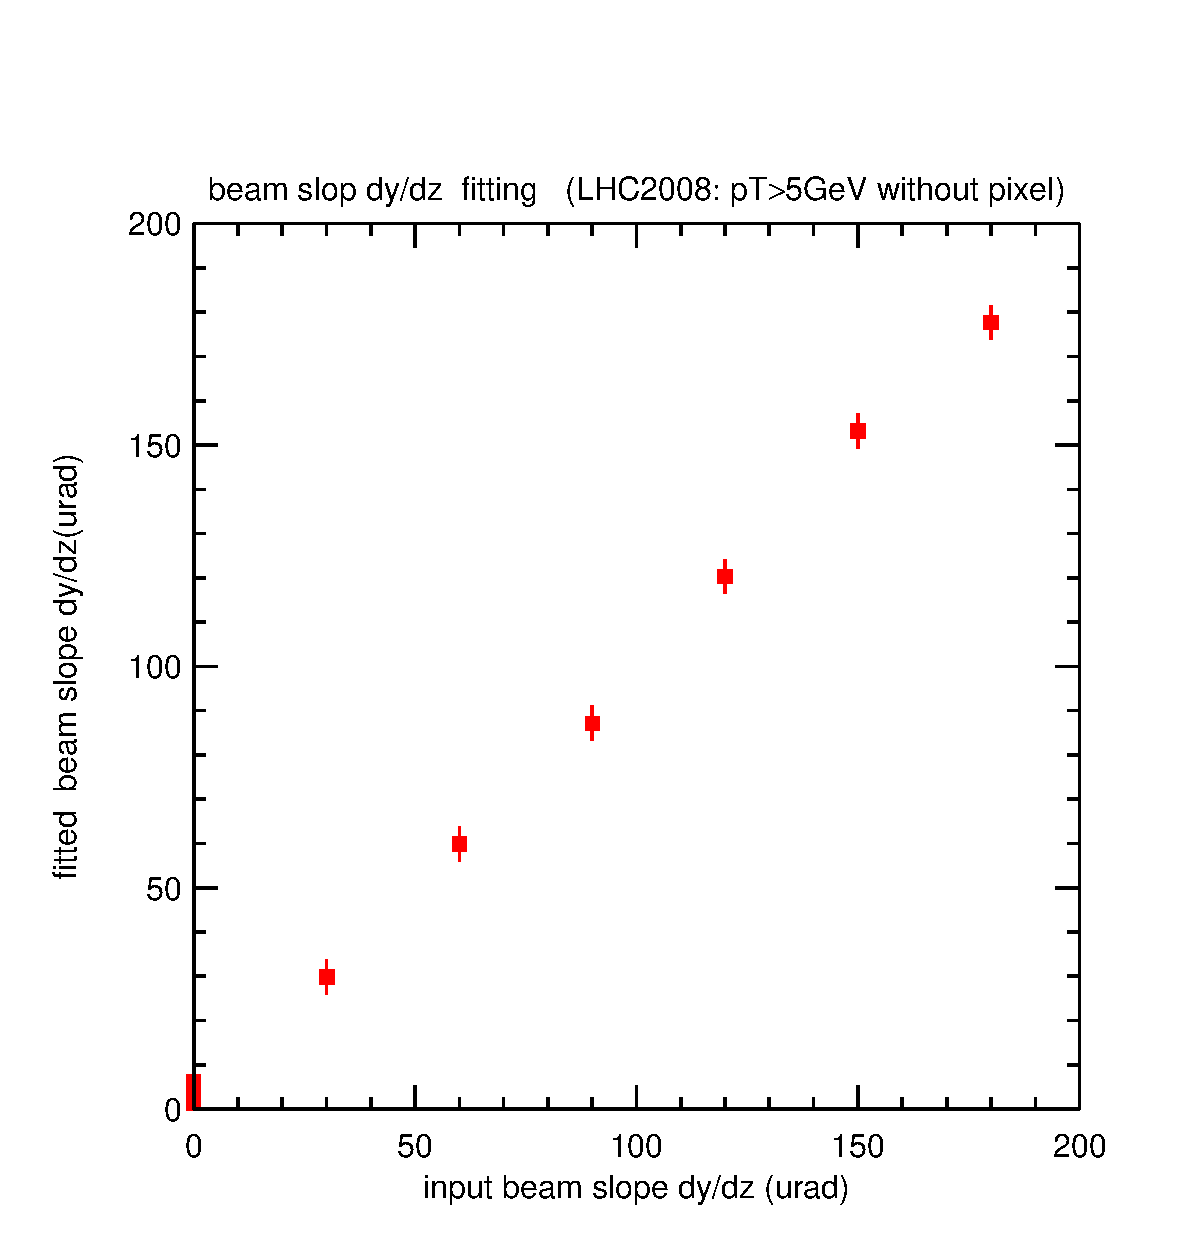
\includegraphics{figures/beam_yslope_fit_nopixel.eps}}
%    \label{fig:BeamSpotNopixelLHC2008}
%    \caption{\it Beam Position fitting result without pixel in CMS tracker in LHC 2008 stable runs. Results
%    from Table \ref{table:BeamSpotNopixelLHC2008}.}
%  \end{center}
%\end{figure}


%\begin{table} [th]
%\begin{center}
%\begin{tabular}{|c|c|c|c|c|c|c|c|} \hline
%\multicolumn{4}{|c|}{Input values}& \multicolumn{4}{|c|}{Fitted  values}\\ \hline
%$z_0$&$\sigma_z$&$\epsilon$ &$\beta^*$  &   $z_0$(Fit)&$\sigma_z$(Fit) &$\epsilon$(Fit)&$\beta^*$(Fit)\\ \hline
%0  &  0  &  0   &  0 & $ 0.31   \pm  0.30 $&$-0.06   \pm  0.30 $&$-1.2 \pm 2.6 $&$1.3\pm  2.6 $ \\ \hline
%100  &  300&  0 &    0 &$  100.32  \pm 0.30$&$ 300.07 \pm  0.29$&$ 2.4 \pm  2.6$&$ -2.4 \pm 2.6 $\\ \hline
%300 &  600&  0  &   0 &$  300.29  \pm 0.30 $&$600.06 \pm  0.29$&$ 5.1 \pm  2.6 $&$-3.9\pm  2.6 $\\ \hline
%600 &  900 & 0  &   0&$   600.02  \pm 0.30$&$ 899.35 \pm  0.30 $&$1.6 \pm  2.6 $&$1.8 \pm  2.6 $\\ \hline
%900 &  1200& 0  &   0&$   900.02  \pm 0.30$&$ 1199.35\pm   0.30$&$ 1.6 \pm  2.6 $&$1.8 \pm  2.6 $\\ \hline
%1200 & 1500& 0  &   0 &$  1200.0  \pm 0.30$&$ 1499.35\pm   0.30 $&$1.6 \pm  2.6$&$ 1.8 \pm  2.6 $\\ \hline
%1500 & 2000& 0  &   0 &$  1500.0   \pm0.30$&$ 1999.35 \pm  0.30$&$ 1.6 \pm  2.6$&$ 1.8  \pm 2.6 $\\ \hline
%2000 & 3000& 0  &   0&$   2000.29  \pm0.30$&$ 3000.06 \pm  0.30$&$ 5.0 \pm  2.6$&$ -3.8 \pm 2.6 $\\ \hline
%3000& 4000& 0  &   0 &$  3000.31 \pm 0.30$&$ 4000.08 \pm     0.29$&$ 2.4 \pm  2.6 $&$-2.6 \pm 2.6 $\\ \hline
%4000& 5000& 0  &   0&$   4000.02 \pm 0.30$&$ 4999.35\pm   0.30$&$ 2.1  \pm 3.9 $&$2.8  \pm 3.9 $\\ \hline
%300&  600&  10 &   30&$  300.02  \pm 0.30$&$ 599.35\pm   0.30$&$ 11.6 \pm  2.6 $&$ 31.8\pm  2.6 $\\ \hline
%300&  600 & 30 &   60&$  300.29 \pm  0.30$&$ 600.06\pm   0.29$&$ 35.1  \pm 2.6 $&$56.1 \pm  2.6 $\\ \hline
%300&  600 & 60 &   90&$  300.31  \pm 0.30$&$ 600.07\pm   0.29$&$ 62.4 \pm  2.6 $&$87.6  \pm 2.6 $\\ \hline
%300 & 600 & 90 &  120&$  300.32  \pm 0.30$&$ 599.94\pm   0.30$&$ 88.8  \pm 2.6$&$ 121.3 \pm 2.6 $\\ \hline
%300 & 600& 120 &  150&$  299.78  \pm 0.30$&$ 599.89  \pm 0.29$&$ 118.5 \pm 2.6 $&$151.5  \pm 2.6 $\\ \hline
%300 & 600 &150 &  180&$  300.02 \pm  0.30$&$ 599.89 \pm  0.30$&$ 152.3  \pm 2.6 $&$180.4 \pm  2.6 $\\ \hline
%300 & 600& 180 &  210&$  300.32  \pm 0.30$&$ 599.68 \pm  0.29$&$ 178.0  \pm 2.6 $&$207.7 \pm   2.6 $\\ \hline
%\end{tabular}
%\caption{\it \label{table:BeamSpotNopixelLHC2007} Beam Position fitting result using tracks 
%from CMS detector configuration without pixel.  Beam profile were generated using 
%parameters $\beta^* =  200~cm$, $\epsilon=3.75 \times 10^{-8}$ and $\sigma_z=11.24~cm$ as 
%expected for LHC 2007 startup runs. About 350K tracks with $p_T>5$~GeV/c were used 
%in each fit.}
%\end{center}
%\end{table}

%\begin{figure}[hbtp]
%  \begin{center} 
%    \resizebox{6cm}{!}{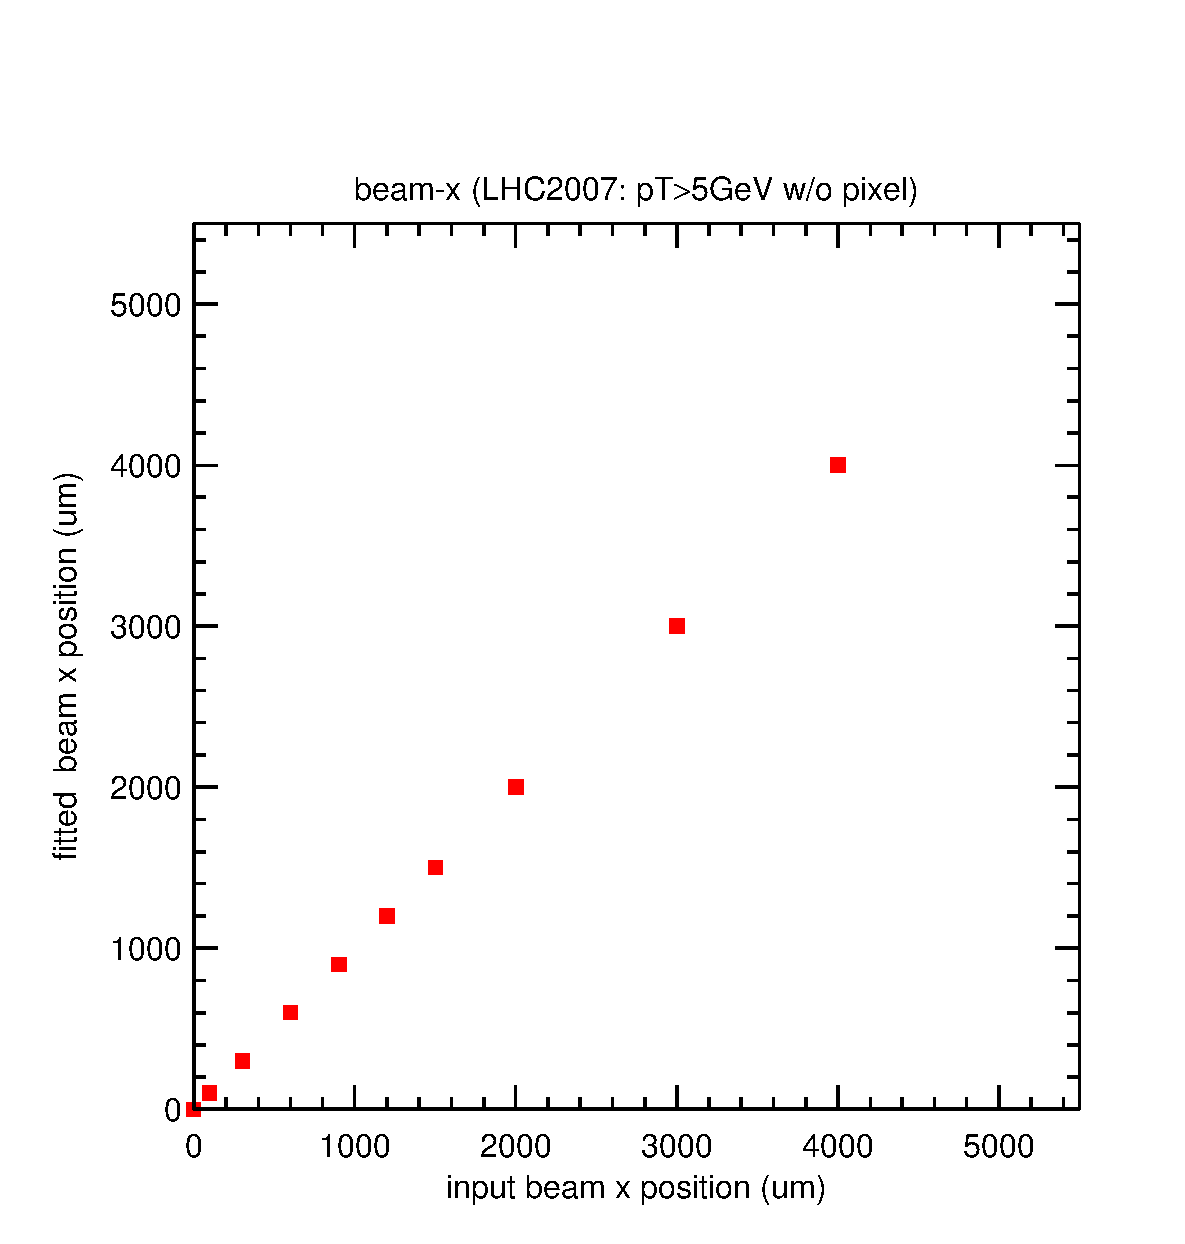
\includegraphics{figures/beam_x_fit_nopixel_LHC2007.eps}}
%    \resizebox{6cm}{!}{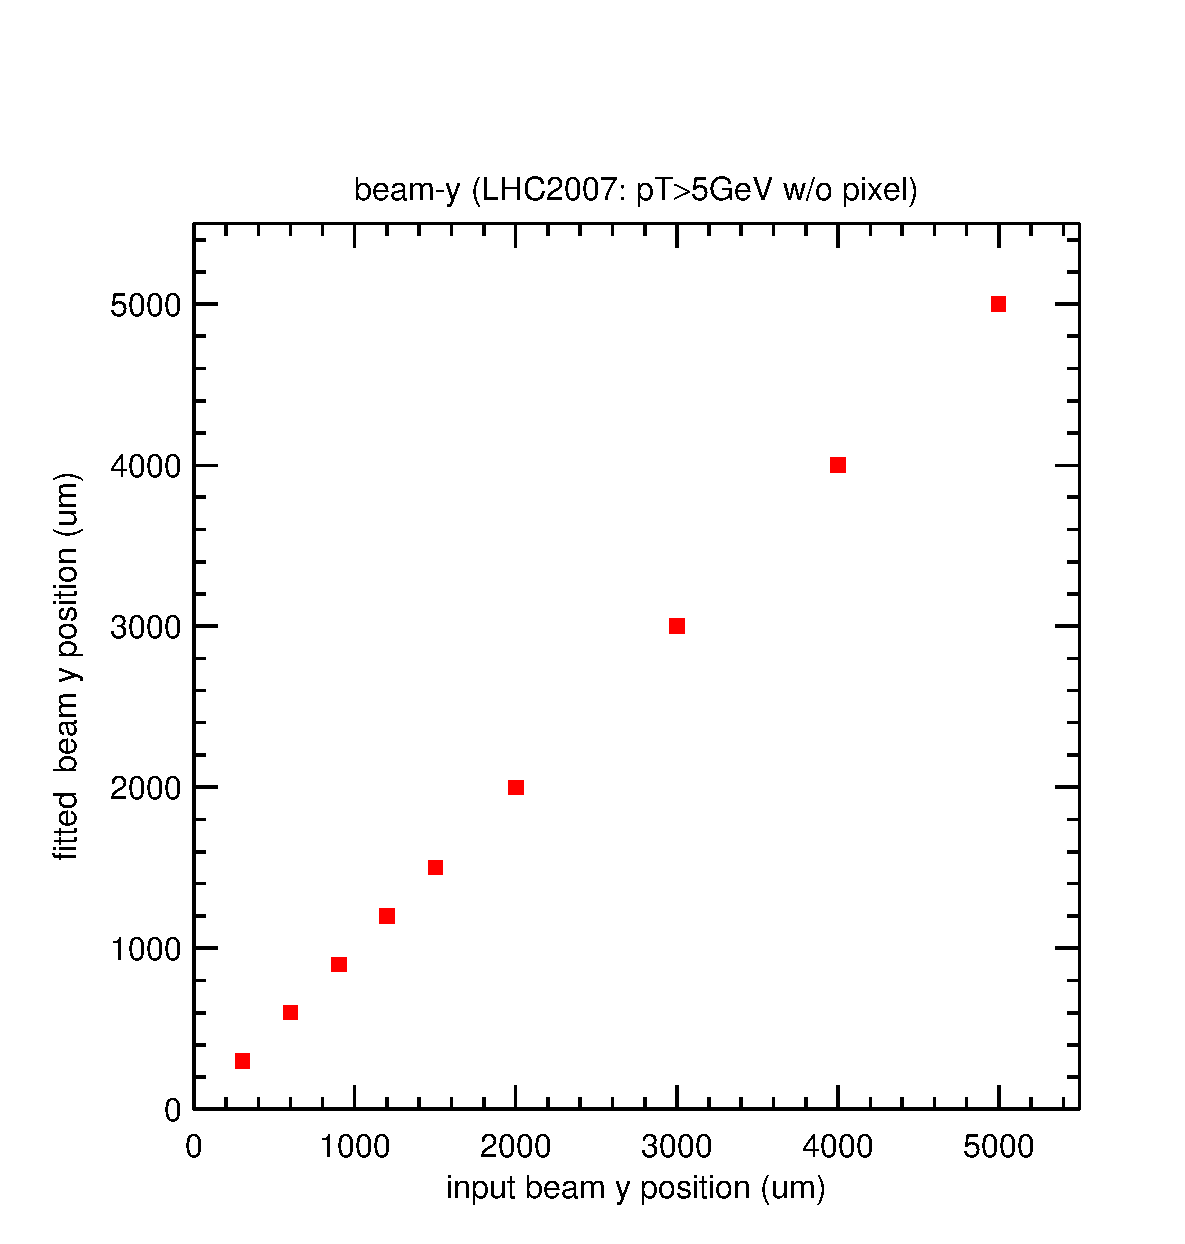
\includegraphics{figures/beam_y_fit_nopixel_LHC2007.eps}}
%    \resizebox{6cm}{!}{\includegraphics{figures/beam_xslope_fit_nopixel_LHC2007.eps}}
%    \resizebox{6cm}{!}{\includegraphics{figures/beam_yslope_fit_nopixel_LHC2007.eps}}
%    \label{fig:BeamSpotNopixelLHC2007}
%    \caption{\it Beam Position fitting result without pixel in CMS tracker in LHC 2007 start-up runs. }
%  \end{center}
%\end{figure}

\clearpage
{\Large \bf Appendix 2}


Below are the  \pythia control cards for minimum bias events and for QCD events with minimal  parton $E_T$ of 50 GeV/c.:


{\small \it
pythia$->$SetMSEL(1);         // select all processes (aka Min Bias)\\
pythia$->$SetMSTP(51,7);      // select CTEQ 5L structure function\\
pythia$->$SetMSTP(81,0);      // switch off mutiple interactions\\
pythia$->$SetMSTJ(22,2);      // Decay those unstable particles\\
pythia$->$SetPARJ(71,10.);    // for which c*tau $<$ 10 mm;\\
pythia$->$SetMSTP(33,3);      // include k-factor\\
pythia$->$SetPARP(82,3.20);   // cut-off pt for multiple interaction\\
pythia$->$SetPARP(89,1960.);\\
pythia$->$SetMSTJ(11,3);      // select fragmentation function "Bowler"\\
pythia$->$SetMSTP(61,1);      // master switch for initial state QED and QCD ra
diation\\
pythia$->$SetMSTP(71,1);      // master switch for final   state QED and QCD ra
diation\\
// uncomment the next 2 line line to set kinematic cuts:\\
//pythia$->$SetCKIN(3,50.);\\
//pythia$->$SetKSEL(0);\\
pythia$->$Initialize("cms", "p", "p", 14000);\\
} 



\clearpage 
\begin{thebibliography}{9}

\bibitem{PhysTDCVol1}
CERN/LHCC 2006-001, CMS Physics TDR Vol 1.

\bibitem{ANAL} There are many examples where the beam was used as an estimate for the primary interaction vertex. 
Two examples are: \\
``Measurement of the Average Lifetime of $B$ hadrons produced in $\bar{\rm p}$p  collisions at
$\sqrt{s}=$ 1.8 TeV", 
F. Abe {\it et al.}, The CDF Collaboration, Phys. Rev. Lett. {\bf 71}, 3421 (1993).

``Measurement of B Hadron Lifetimes Using $J/\psi$ Final States at CDF",
F. Abe {\it et al.}, The CDF Collaboration, Phys. Rev. {\bf D57}, 5382 (1998).

\bibitem{NIM} ``The Silicon Detector of the Collider Detector at Fermilab.'' 
              Nuclear Instruments and methods in Physics Research A 350 (1994) p 73-130.

\bibitem {damage} ``CDF Run 2A Silicon Detector Damage. Assessment.'' G. Bolla et al.\\ 
``http://www-cdf.fnal.gov/upgrades/run2b/P5\_Mar03/damage.ps''

\bibitem {BEAMPHYSIC} {Beam Physics Note 63  25/04/02},
    B. Muratori,  {\em "Luminosity Considerations for the LHC"}.

\bibitem {BEAMCON}
    W. Herr, B. Muratori,  {\em "Concept of Luminosity"}. Prepared for CERN Accelerator School and DESY Zeuthen:
Accelerator Physics, Zeuthen, Germany, 15-26 Sep 2003
``http://lhc-beam-beam.web.cern.ch/lhc-beam-beam/papers/lum.ps''\\
``http://cas.web.cern.ch/cas/Trieste-2005/Lectures-pdf/Herr-luminosity.pdf''.


\bibitem{RunII}
``Tevatron Run II Luminosity, Emittance and Collision Point''\\
J. Slaughter, J. Estrada, K. Genser, A. Jansson, P. Lebrun, J.
C. Yun, S. Lai\\
Particle Accelerator Conference, 2003. PAC 2003. Proceedings of the
Volume 3, Issue , 12-16 May 2003 Page(s): 1763 - 1765 Vol. 3.

\bibitem{IPnopixel}
B. Mangano, "The CMS Tracker: contributions to hardware integration, software development and first data taking", Ph.D. thesis in preparation. 
%, ``Tracking without pixels '', talk at the January  2006 FNAL Tracker Software Workshop. 
%``http://indico.cern.ch/materialDisplay.py?contribId=s5t2\&amp;sessionId=s5\&amp;materialId=0\&amp;confId=a058113''


\bibitem {RunIIBeam} 
V. Shiltsev {\em et al.}, Phys. Rev. ST Accel. Beams 8, 101001 (2005).


\bibitem{handbook}
RUN II Handbook ``http://www-bd.fnal.gov/runII/index.html''.



\bibitem{LHCBeam}
``http://lhc.web.cern.ch/lhc/'' under ``Beam Parameter''.


\bibitem{pythia6}
%For the \pythia-6 installation in FNAL CMS UAF, contact H. Wenzel 
%or check the ROOT page:
``http://root.cern.ch/root/html/TPythia6.html''.

\bibitem{pythia}
T. Sjostrand, L. Lonnblad, and S. Mrenna, ``PYTHIA 6.2: Physics and manual'', arXiv:hep-ph/0108264.
``http://www.thep.lu.se/~torbjorn/Pythia.html''.


 


%\bibitem{datacards}
%We used the following data cards to generate Minimum Bias Events:\\
%%\begin{verbatim}
%{\small \it
%pythia$->$SetMSEL(1);         // select all processes (aka Min Bias)\\
%pythia$->$SetMSTP(51,7);      // select CTEQ 5L structure function\\
%pythia$->$SetMSTP(81,0);      // switch off mutiple interactions\\
%pythia$->$SetMSTJ(22,2);      // Decay those unstable particles\\
%pythia$->$SetPARJ(71,10.);    // for which c*tau $<$ 10 mm;\\
%pythia$->$SetMSTP(33,3);      // include k-factor\\
%pythia$->$SetPARP(82,3.20);   // cut-off pt for multiple interaction\\
%pythia$->$SetPARP(89,1960.);\\
%pythia$->$SetMSTJ(11,3);      // select fragmentation function "Bowler"\\
%pythia$->$SetMSTP(61,1);      // master switch for initial state QED and QCD radiation\\
%pythia$->$SetMSTP(71,1);      // master switch for final   state QED and QCD radiation\\
%// uncomment the next 2 line line to set kinematic cuts:\\
%//pythia$->$SetCKIN(3,50.);\\
%//pythia$->$SetKSEL(0);\\
%pythia$->$Initialize("cms", "p", "p", 14000);\\
%}
%\end{verbatim} 




\bibitem {CTF}
W. Adam et al., ``Track reconstruction in the CMS tracker'', CMS Note 2006/041 (2006).


\bibitem {VtxSmearingPkg}
IOMC/EventVertexGenerators package within the CMS software reconstruction, 

``http://cmssw.cvs.cern.ch/cgi-bin/cmssw.cgi/CMSSW/IOMC/EventVertexGenerators/?cvsroot=CMSSW''.

\bibitem{BeamSpotProducer}
The $d_0 - \varphi_0$ and log-likelihood fits have been implemented in a package
within the CMS software reconstruction. This package also includes a class object (BeamSpot) that holds all the beam information: 
XYZ beam position, two slopes, RMS beam length, beam width, and a full covariance matrix. This
object can be used to store the beam information in the database.
The fits available are: $\chi^2$ and log-likelihood fits for $z$-distribution,
$d_0 - \varphi_0$ fitter, log-likelihood fit for beam position and  
log-likelihood fit for extraction of the beam width. The likelihood fitters have been implemented
using MINUIT2.

\bibitem {CVS} 
``http://cdcvs.fnal.gov/cgi-bin/public-cvs/cvsweb-public.cgi/beamfit/?cvsroot=lpc''.

\bibitem {oldCMSnote}
M. Vos and F. Palla, ``b-tagging in the High Level Trigger'', CMS Note 2006/030 (2006).

%\bibitem {Datasets}
%These are official data samples as reported by the CMS data discovery page DBS:\\
%''http://cmsdbs.cern.ch/discovery/''.

%{{ \it "The Primary Interaction Vertex",}}
%{\small Hans Wenzel};
%CDF Note {\bf 4066}, Nov. 1997





\end{thebibliography}

%------------------------------------------------------------------------------

 
\end{document}
